\chapter{The Unified Coordinate System}
\label{chpt:UCS}

Insert text here

\section{Background}
\label{sec:UCS-background}

Insert text here

\section{The Euler Equations in Unified Coordinates}
\label{sec:UCS-Euler}

We here present the method for deriving the Unified Coordinate System (UCS) transformation, and we also show how to transform the conservation form of the Euler equations from Cartesian coordinate to UCS coordinates. In all of the following, implied sums over greek indices are to be taken over four-dimensional space-time,  and sums over latin indices are to be taken over three-dimensional space.

\subsection{The Unified Coordinate System}
\label{sec:UCS-UCS-derivation}
UCS is defined by the coordinate transformation:
\begin{equation}
\label{eq:UCS-transformation}
% MathType!MTEF!2!1!+-
% faaagCart1ev2aaaKnaaaaWenf2ys9wBH5garuavP1wzZbqedmvETj
% 2BSbqefm0B1jxALjharqqtubsr4rNCHbGeaGqiVu0Je9sqqrpepC0x
% bbL8FesqqrFfpeea0xe9Lq-Jc9vqaqpepm0xbba9pwe9Q8fs0-yqaq
% pepae9pg0FirpepeKkFr0xfr-xfr-xb9Gqpi0dc9adbaqaaeGaciGa
% aiaabeqaamaabaabaaGcbaWaamWaaeaafaWabeabbaaaaeaacaWGKb
% GaamiDaaqaaiaadsgacaWG4baabaGaamizaiaadMhaaeaacaWGKbGa
% amOEaaaaaiaawUfacaGLDbaacqGH9aqpdaWadaqaauaadeqaeqaaaa
% aabaGaaGymaaqaaiaaicdaaeaacaaIWaaabaGaaGimaaqaaiaadwfa
% aeaacaWGbbaabaGaamitaaqaaiaadcfaaeaacaWGwbaabaGaamOqaa
% qaaiaad2eaaeaacaWGrbaabaGaam4vaaqaaiaadoeaaeaacaWGobaa
% baGaamOuaaaaaiaawUfacaGLDbaacqGHflY1daWadaqaauaadeqaee
% aaaaqaaiaadsgacqaH7oaBaeaacaWGKbGaeqOVdGhabaGaamizaiab
% eE7aObqaaiaadsgacqaH2oGEaaaacaGLBbGaayzxaaaaaa!5669!
\left[ {\begin{array}{*{20}{c}}
{dt}\\
{dx}\\
{dy}\\
{dz}
\end{array}} \right] = \left[ {\begin{array}{*{20}{c}}
1&0&0&0\\
U&A&L&P\\
V&B&M&Q\\
W&C&N&R
\end{array}} \right] \cdot \left[ {\begin{array}{*{20}{c}}
{d\lambda }\\
{d\xi }\\
{d\eta }\\
{d\zeta }
\end{array}} \right]
\end{equation}

\ref{eq:UCS-transformation} may be written more succinctly as 
% MathType!MTEF!2!1!+-
% faaagCart1ev2aaaKnaaaaWenf2ys9wBH5garuavP1wzZbqedmvETj
% 2BSbqefm0B1jxALjharqqtubsr4rNCHbGeaGqiVu0Je9sqqrpepC0x
% bbL8FesqqrFfpeea0xe9Lq-Jc9vqaqpepm0xbba9pwe9Q8fs0-yqaq
% pepae9pg0FirpepeKkFr0xfr-xfr-xb9Gqpi0dc9adbaqaaeGaciGa
% aiaabeqaamaabaabaaGcbaGaamizaiaadIhadaWgaaWcbaGaeqySde
% gabeaakiabg2da9maalaaabaGaeyOaIyRaamiEamaaBaaaleaacqaH
% XoqyaeqaaaGcbaGaeyOaIyRaeqOVdG3aaWbaaSqabeaacqaHYoGyaa
% aaaOGaamizaiabe67a4naaBaaaleaacqaHYoGyaeqaaaaa!409C!
$d{x_\alpha } = \frac{{\partial {x_\alpha }}}{{\partial {\xi ^\beta
}}}d{\xi _\beta }$, which naturally leads to the corresponding
transformation for vectors and derivatives which can be written as
% MathType!MTEF!2!1!+-
% faaagCart1ev2aaaKnaaaaWenf2ys9wBH5garuavP1wzZbqedmvETj
% 2BSbqefm0B1jxALjharqqtubsr4rNCHbGeaGqiVu0Je9sqqrpepC0x
% bbL8FesqqrFfpeea0xe9Lq-Jc9vqaqpepm0xbba9pwe9Q8fs0-yqaq
% pepae9pg0FirpepeKkFr0xfr-xfr-xb9Gqpi0dc9adbaqaaeGaciGa
% aiaabeqaamaabaabaaGcbaWaaSaaaeaacqGHciITaeaacqGHciITca
% WG4bWaaWbaaSqabeaacqaHXoqyaaaaaOGaeyypa0ZaaSaaaeaacqGH
% ciITcqaH+oaEdaWgaaWcbaGaeqOSdigabeaaaOqaaiabgkGi2kaadI
% hadaahaaWcbeqaaiabeg7aHbaaaaGcdaWcaaqaaiabgkGi2cqaaiab
% gkGi2kabe67a4naaCaaaleqabaGaeqOSdigaaaaaaaa!4484!
$\frac{\partial }{{\partial {x^\alpha }}} = \frac{{\partial {\xi
      _\beta }}}{{\partial {x^\alpha }}}\frac{\partial }{{\partial
    {\xi ^\beta }}}$, or in expanded form as:
\begin{equation}
\label{eq:UCS-vector-transformation}
% MathType!MTEF!2!1!+-
% faaagCart1ev2aaaKnaaaaWenf2ys9wBH5garuavP1wzZbqedmvETj
% 2BSbqefm0B1jxALjharqqtubsr4rNCHbGeaGqiVu0Je9sqqrpepC0x
% bbL8FesqqrFfpeea0xe9Lq-Jc9vqaqpepm0xbba9pwe9Q8fs0-yqaq
% pepae9pg0FirpepeKkFr0xfr-xfr-xb9Gqpi0dc9adbaqaaeGaciGa
% aiaabeqaamaabaabaaGcbaWaamWaaeaafaWabeabbaaaaeaadaWcaa
% qaaiabgkGi2cqaaiabgkGi2kaadshaaaaabaWaaSaaaeaacqGHciIT
% aeaacqGHciITcaWG4baaaaqaamaalaaabaGaeyOaIylabaGaeyOaIy
% RaamyEaaaaaeaadaWcaaqaaiabgkGi2cqaaiabgkGi2kaadQhaaaaa
% aaGaay5waiaaw2faaiabg2da9maadmaabaqbamqabqabaaaaaeaaca
% aIXaaabaGaeyOeI0IaamyvamaaBaaaleaacqaH+oaEaeqaaaGcbaGa
% eyOeI0IaamyvamaaBaaaleaacqaH3oaAaeqaaaGcbaGaeyOeI0Iaam
% yvamaaBaaaleaacqaH2oGEaeqaaaGcbaGaaGimaaqaamaalaaabaGa
% amytaiaadkfacqGHsislcaWGobGaamyuaaqaaiaadQeaaaaabaWaaS
% aaaeaacaWGdbGaamyuaiabgkHiTiaadkeacaWGsbaabaGaamOsaaaa
% aeaadaWcaaqaaiaadkeacaWGobGaeyOeI0Iaam4qaiaad2eaaeaaca
% WGkbaaaaqaaiaaicdaaeaadaWcaaqaaiaad6eacaWGqbGaeyOeI0Ia
% amitaiaadkfaaeaacaWGkbaaaaqaamaalaaabaGaamyqaiaadkfacq
% GHsislcaWGdbGaamiuaaqaaiaadQeaaaaabaWaaSaaaeaacaWGdbGa
% amitaiabgkHiTiaadgeacaWGobaabaGaamOsaaaaaeaacaaIWaaaba
% WaaSaaaeaacaWGmbGaamyuaiabgkHiTiaad2eacaWGqbaabaGaamOs
% aaaaaeaadaWcaaqaaiaadkeacaWGqbGaeyOeI0Iaamyqaiaadgfaae
% aacaWGkbaaaaqaamaalaaabaGaamyqaiaad2eacqGHsislcaWGcbGa
% amitaaqaaiaadQeaaaaaaaGaay5waiaaw2faaiabgwSixpaadmaaba
% qbamqabqqaaaaabaWaaSaaaeaacqGHciITaeaacqGHciITcqaH7oaB
% aaaabaWaaSaaaeaacqGHciITaeaacqGHciITcqaH+oaEaaaabaWaaS
% aaaeaacqGHciITaeaacqGHciITcqaH3oaAaaaabaWaaSaaaeaacqGH
% ciITaeaacqGHciITcqaH2oGEaaaaaaGaay5waiaaw2faaaaa!94A6!
\left[ {\begin{array}{*{20}{c}}
{\frac{\partial }{{\partial t}}}\\
{\frac{\partial }{{\partial x}}}\\
{\frac{\partial }{{\partial y}}}\\
{\frac{\partial }{{\partial z}}}
\end{array}} \right] = \left[ {\begin{array}{*{20}{c}}
1&{ - {U_\xi }}&{ - {U_\eta }}&{ - {U_\zeta }}\\
0&{\frac{{MR - NQ}}{J}}&{\frac{{CQ - BR}}{J}}&{\frac{{BN - CM}}{J}}\\
0&{\frac{{NP - LR}}{J}}&{\frac{{AR - CP}}{J}}&{\frac{{CL - AN}}{J}}\\
0&{\frac{{LQ - MP}}{J}}&{\frac{{BP - AQ}}{J}}&{\frac{{AM - BL}}{J}}
\end{array}} \right] \cdot \left[ {\begin{array}{*{20}{c}}
{\frac{\partial }{{\partial \lambda }}}\\
{\frac{\partial }{{\partial \xi }}}\\
{\frac{\partial }{{\partial \eta }}}\\
{\frac{\partial }{{\partial \zeta }}}
\end{array}} \right]
\end{equation}
In Eq.~\ref{eq:UCS-vector-transformation}, we have defined the following relations:

% MathType!MTEF!2!1!+-
% faaagCart1ev2aaaKnaaaaWenf2ys9wBH5garuavP1wzZbqedmvETj
% 2BSbqefm0B1jxALjharqqtubsr4rNCHbGeaGqiVu0Je9sqqrpepC0x
% bbL8FesqqrFfpeea0xe9Lq-Jc9vqaqpepm0xbba9pwe9Q8fs0-yqaq
% pepae9pg0FirpepeKkFr0xfr-xfr-xb9Gqpi0dc9adbaqaaeGaciGa
% aiaabeqaamaabaabaaGceaqabeaacaWGvbWaaSbaaSqaaiabe67a4n
% aaBaaameaacaWGPbaabeaaaSqabaGccqGHHjIUdaqadaqaaiaadwfa
% caGGSaGaamOvaiaacYcacaWGxbaacaGLOaGaayzkaaGaeyyXICTaey
% 4bIe9aaSbaaSqaaiqadIhagaWcaaqabaGccqaH+oaEdaWgaaWcbaGa
% amyAaaqabaaakeaacqGHhis0daWgaaWcbaGabmiEayaalaaabeaaki
% abe67a4jabggMi6oaalaaabaGaaGymaaqaaiaadQeaaaWaaeWaaeaa
% caWGnbGaamOuaiabgkHiTiaad6eacaWGrbGaaiilaiaad6eacaWGqb
% GaeyOeI0IaamitaiaadkfacaGGSaGaamitaiaadgfacqGHsislcaWG
% nbGaamiuaaGaayjkaiaawMcaaaqaaiabgEGirpaaBaaaleaaceWG4b
% GbaSaaaeqaaOGaeq4TdGMaeyyyIO7aaSaaaeaacaaIXaaabaGaamOs
% aaaadaqadaqaaiaadoeacaWGrbGaeyOeI0IaamOqaiaadkfacaGGSa
% GaamyqaiaadkfacqGHsislcaWGdbGaamiuaiaacYcacaWGcbGaamiu
% aiabgkHiTiaadgeacaWGrbaacaGLOaGaayzkaaaabaGaey4bIe9aaS
% baaSqaaiqadIhagaWcaaqabaGccqaH2oGEcqGHHjIUdaWcaaqaaiaa
% igdaaeaacaWGkbaaamaabmaabaGaamOqaiaad6eacqGHsislcaWGdb
% GaamytaiaacYcacaWGdbGaamitaiabgkHiTiaadgeacaWGobGaaiil
% aiaadgeacaWGnbGaeyOeI0IaamOqaiaadYeaaiaawIcacaGLPaaaaa
% aa!8754!
\[\begin{array}{l}
{U_{{\xi _i}}} \equiv \left( {U,V,W} \right) \cdot {\nabla _{\vec x}}{\xi _i}\\
{\nabla _{\vec x}}\xi  \equiv \frac{1}{J}\left( {MR - NQ,NP - LR,LQ - MP} \right)\\
{\nabla _{\vec x}}\eta  \equiv \frac{1}{J}\left( {CQ - BR,AR - CP,BP - AQ} \right)\\
{\nabla _{\vec x}}\zeta  \equiv \frac{1}{J}\left( {BN - CM,CL - AN,AM - BL} \right)
\end{array}\]

% MathType!MTEF!2!1!+-
% faaagCart1ev2aaaKnaaaaWenf2ys9wBH5garuavP1wzZbqedmvETj
% 2BSbqefm0B1jxALjharqqtubsr4rNCHbGeaGqiVu0Je9sqqrpepC0x
% bbL8FesqqrFfpeea0xe9Lq-Jc9vqaqpepm0xbba9pwe9Q8fs0-yqaq
% pepae9pg0FirpepeKkFr0xfr-xfr-xb9Gqpi0dc9adbaqaaeGaciGa
% aiaabeqaamaabaabaaGcbaGaamOsaiabggMi6oaaemaabaqbamqabm
% WaaaqaaiaadgeaaeaacaWGmbaabaGaamiuaaqaaiaadkeaaeaacaWG
% nbaabaGaamyuaaqaaiaadoeaaeaacaWGobaabaGaamOuaaaaaiaawE
% a7caGLiWoacqGH9aqpcqaH1oqzdaWgaaWcbaGaamyAaiaadQgacaWG
% RbaabeaakiaadgeadaWgaaWcbaGaamyAaaqabaGccaWGmbWaaSbaaS
% qaaiaadQgaaeqaaOGaamiuamaaBaaaleaacaWGRbaabeaaaaa!46BA!
\[J \equiv \left| {\begin{array}{*{20}{c}}
A&L&P\\
B&M&Q\\
C&N&R
\end{array}} \right| = {\varepsilon _{ijk}}{A_i}{L_j}{P_k}\]

% MathType!MTEF!2!1!+-
% faaagCart1ev2aaaKnaaaaWenf2ys9wBH5garuavP1wzZbqedmvETj
% 2BSbqefm0B1jxALjharqqtubsr4rNCHbGeaGqiVu0Je9sqqrpepC0x
% bbL8FesqqrFfpeea0xe9Lq-Jc9vqaqpepm0xbba9pwe9Q8fs0-yqaq
% pepae9pg0FirpepeKkFr0xfr-xfr-xb9Gqpi0dc9adbaqaaeGaciGa
% aiaabeqaamaabaabaaGcbaGabmyvayaalaGaeyyyIO7aaeWaaeaaca
% WGvbGaaiilaiaadAfacaGGSaGaam4vaaGaayjkaiaawMcaaiaacUda
% caaMc8UaaGPaVlaaykW7ceWGbbGbaSaacqGHHjIUdaqadaqaaiaadg
% eacaGGSaGaamOqaiaacYcacaWGdbaacaGLOaGaayzkaaGaai4oaiaa
% ykW7caaMc8UaaGPaVlaadYeacqGHHjIUdaqadaqaaiaadYeacaGGSa
% GaamytaiaacYcacaWGobaacaGLOaGaayzkaaGaai4oaiaaykW7caaM
% c8UabmiuayaalaGaeyyyIO7aaeWaaeaacaWGqbGaaiilaiaadgfaca
% GGSaGaamOuaaGaayjkaiaawMcaaaaa!5CD0!
\[\vec U \equiv \left( {U,V,W} \right);\,\,\,\vec A \equiv \left( {A,B,C} \right);\,\,\,L \equiv \left( {L,M,N} \right);\,\,\vec P \equiv \left( {P,Q,R} \right)\]

In particular, the above definitions provide the formulas for projection of a vector in global Cartesian coordinates onto the computational coordinate vectors, as well as providing a useful shorthand for later derivations.

The UCS transformation in Eq.~\ref{eq:UCS-transformation} is not complete as written, however. In order for the transformation to be well-behaved, it is necessary to impose additional conditions on the components of the transformation. In particular, it is necessary that partial derivatives commute:
% MathType!MTEF!2!1!+-
% faaagCart1ev2aaaKnaaaaWenf2ys9wBH5garuavP1wzZbqedmvETj
% 2BSbqefm0B1jxALjharqqtubsr4rNCHbGeaGqiVu0Je9sqqrpepC0x
% bbL8FesqqrFfpeea0xe9Lq-Jc9vqaqpepm0xbba9pwe9Q8fs0-yqaq
% pepae9pg0FirpepeKkFr0xfr-xfr-xb9Gqpi0dc9adbaqaaeGaciGa
% aiaabeqaamaabaabaaGcbaWaaSaaaeaacqGHciITaeaacqGHciITcq
% aH+oaEdaahaaWcbeqaaiabeo7aNbaaaaGcdaqadaqaamaalaaabaGa
% eyOaIyRaamiEamaaBaaaleaacqaHXoqyaeqaaaGcbaGaeyOaIyRaeq
% OVdG3aaWbaaSqabeaacqaHYoGyaaaaaaGccaGLOaGaayzkaaGaeyyp
% a0ZaaSaaaeaacqGHciITaeaacqGHciITcqaH+oaEdaahaaWcbeqaai
% abek7aIbaaaaGcdaqadaqaamaalaaabaGaeyOaIyRaamiEamaaBaaa
% leaacqaHXoqyaeqaaaGcbaGaeyOaIyRaeqOVdG3aaWbaaSqabeaacq
% aHZoWzaaaaaaGccaGLOaGaayzkaaaaaa!51BD!
\[\frac{\partial }{{\partial {\xi ^\gamma }}}\left( {\frac{{\partial {x_\alpha }}}{{\partial {\xi ^\beta }}}} \right) = \frac{\partial }{{\partial {\xi ^\beta }}}\left( {\frac{{\partial {x_\alpha }}}{{\partial {\xi ^\gamma }}}} \right)\]

Upon expansion, and using the notation of Eq.~\ref{eq:UCS-transformation}, this constraint is equivalent to the following compatibility conditions:

\begin{equation}
\label{eq:compatibility-conditions}
% MathType!MTEF!2!1!+-
% faaagCart1ev2aaaKnaaaaWenf2ys9wBH5garuavP1wzZbqedmvETj
% 2BSbqefm0B1jxALjharqqtubsr4rNCHbGeaGqiVu0Je9sqqrpepC0x
% bbL8FesqqrFfpeea0xe9Lq-Jc9vqaqpepm0xbba9pwe9Q8fs0-yqaq
% pepae9pg0FirpepeKkFr0xfr-xfr-xb9Gqpi0dc9adbaqaaeGaciGa
% aiaabeqaamaabaabaaGcbaqbamqabyWaaaaabaWaaSaaaeaacqGHci
% ITcaWGbbaabaGaeyOaIyRaeq4UdWgaaiabg2da9maalaaabaGaeyOa
% IyRaamyvaaqaaiabgkGi2kabe67a4baaaeaadaWcaaqaaiabgkGi2k
% aadYeaaeaacqGHciITcqaH7oaBaaGaeyypa0ZaaSaaaeaacqGHciIT
% caWGvbaabaGaeyOaIyRaeq4TdGgaaaqaamaalaaabaGaeyOaIyRaam
% iuaaqaaiabgkGi2kabeU7aSbaacqGH9aqpdaWcaaqaaiabgkGi2kaa
% dwfaaeaacqGHciITcqaH2oGEaaaabaWaaSaaaeaacqGHciITcaWGcb
% aabaGaeyOaIyRaeq4UdWgaaiabg2da9maalaaabaGaeyOaIyRaamOv
% aaqaaiabgkGi2kabe67a4baaaeaadaWcaaqaaiabgkGi2kaad2eaae
% aacqGHciITcqaH7oaBaaGaeyypa0ZaaSaaaeaacqGHciITcaWGwbaa
% baGaeyOaIyRaeq4TdGgaaaqaamaalaaabaGaeyOaIyRaamyuaaqaai
% abgkGi2kabeU7aSbaacqGH9aqpdaWcaaqaaiabgkGi2kaadAfaaeaa
% cqGHciITcqaH2oGEaaaabaWaaSaaaeaacqGHciITcaWGdbaabaGaey
% OaIyRaeq4UdWgaaiabg2da9maalaaabaGaeyOaIyRaam4vaaqaaiab
% gkGi2kabe67a4baaaeaadaWcaaqaaiabgkGi2kaad6eaaeaacqGHci
% ITcqaH7oaBaaGaeyypa0ZaaSaaaeaacqGHciITcaWGxbaabaGaeyOa
% IyRaeq4TdGgaaaqaamaalaaabaGaeyOaIyRaamOuaaqaaiabgkGi2k
% abeU7aSbaacqGH9aqpdaWcaaqaaiabgkGi2kaadEfaaeaacqGHciIT
% cqaH2oGEaaaabaWaaSaaaeaacqGHciITcaWGbbaabaGaeyOaIyRaeq
% 4TdGgaaiabg2da9maalaaabaGaeyOaIyRaamitaaqaaiabgkGi2kab
% e67a4baaaeaadaWcaaqaaiabgkGi2kaadgeaaeaacqGHciITcqaH2o
% GEaaGaeyypa0ZaaSaaaeaacqGHciITcaWGqbaabaGaeyOaIyRaeqOV
% dGhaaaqaamaalaaabaGaeyOaIyRaamitaaqaaiabgkGi2kabeA7a6b
% aacqGH9aqpdaWcaaqaaiabgkGi2kaadcfaaeaacqGHciITcqaH3oaA
% aaaabaWaaSaaaeaacqGHciITcaWGcbaabaGaeyOaIyRaeq4TdGgaai
% abg2da9maalaaabaGaeyOaIyRaamytaaqaaiabgkGi2kabe67a4baa
% aeaadaWcaaqaaiabgkGi2kaadkeaaeaacqGHciITcqaH2oGEaaGaey
% ypa0ZaaSaaaeaacqGHciITcaWGrbaabaGaeyOaIyRaeqOVdGhaaaqa
% amaalaaabaGaeyOaIyRaamytaaqaaiabgkGi2kabeA7a6baacqGH9a
% qpdaWcaaqaaiabgkGi2kaadgfaaeaacqGHciITcqaH3oaAaaaabaWa
% aSaaaeaacqGHciITcaWGdbaabaGaeyOaIyRaeq4TdGgaaiabg2da9m
% aalaaabaGaeyOaIyRaamOtaaqaaiabgkGi2kabe67a4baaaeaadaWc
% aaqaaiabgkGi2kaadoeaaeaacqGHciITcqaH2oGEaaGaeyypa0ZaaS
% aaaeaacqGHciITcaWGsbaabaGaeyOaIyRaeqOVdGhaaaqaamaalaaa
% baGaeyOaIyRaamOtaaqaaiabgkGi2kabeA7a6baacqGH9aqpdaWcaa
% qaaiabgkGi2kaadkfaaeaacqGHciITcqaH3oaAaaaaaaaa!0314!
\begin{array}{*{20}{c}}
{\frac{{\partial A}}{{\partial \lambda }} = \frac{{\partial U}}{{\partial \xi }}}&{\frac{{\partial L}}{{\partial \lambda }} = \frac{{\partial U}}{{\partial \eta }}}&{\frac{{\partial P}}{{\partial \lambda }} = \frac{{\partial U}}{{\partial \zeta }}}\\
{\frac{{\partial B}}{{\partial \lambda }} = \frac{{\partial V}}{{\partial \xi }}}&{\frac{{\partial M}}{{\partial \lambda }} = \frac{{\partial V}}{{\partial \eta }}}&{\frac{{\partial Q}}{{\partial \lambda }} = \frac{{\partial V}}{{\partial \zeta }}}\\
{\frac{{\partial C}}{{\partial \lambda }} = \frac{{\partial W}}{{\partial \xi }}}&{\frac{{\partial N}}{{\partial \lambda }} = \frac{{\partial W}}{{\partial \eta }}}&{\frac{{\partial R}}{{\partial \lambda }} = \frac{{\partial W}}{{\partial \zeta }}}\\
{\frac{{\partial A}}{{\partial \eta }} = \frac{{\partial L}}{{\partial \xi }}}&{\frac{{\partial A}}{{\partial \zeta }} = \frac{{\partial P}}{{\partial \xi }}}&{\frac{{\partial L}}{{\partial \zeta }} = \frac{{\partial P}}{{\partial \eta }}}\\
{\frac{{\partial B}}{{\partial \eta }} = \frac{{\partial M}}{{\partial \xi }}}&{\frac{{\partial B}}{{\partial \zeta }} = \frac{{\partial Q}}{{\partial \xi }}}&{\frac{{\partial M}}{{\partial \zeta }} = \frac{{\partial Q}}{{\partial \eta }}}\\
{\frac{{\partial C}}{{\partial \eta }} = \frac{{\partial N}}{{\partial \xi }}}&{\frac{{\partial C}}{{\partial \zeta }} = \frac{{\partial R}}{{\partial \xi }}}&{\frac{{\partial N}}{{\partial \zeta }} = \frac{{\partial R}}{{\partial \eta }}}
\end{array}
\end{equation}

The conditions of Eq.~\ref{eq:compatibility-conditions} are not independent. In particular, if the 9 purely spatial conditions are satisfied at some initial time $\lambda$, then it follows that the 9 conditions involving the temporal derivative  $\diff{}{\lambda}$ are sufficient to ensure that the full compatibility conditions will be met at all other times.

\subsection{The Three-dimensional Euler Equations}
\label{sec:UCS-3D-Euler}

The three-dimensional, unsteady, Euler equations are a system of five nonlinear equations defined on four-dimensional space-time ($\mathbb{R}^4$) by the fluxes:

% MathType!MTEF!2!1!+-
% faaagCart1ev2aaaKnaaaaWenf2ys9wBH5garuavP1wzZbqedmvETj
% 2BSbqefm0B1jxALjharqqtubsr4rNCHbGeaGqiVu0Je9sqqrpepC0x
% bbL8FesqqrFfpeea0xe9Lq-Jc9vqaqpepm0xbba9pwe9Q8fs0-yqaq
% pepae9pg0FirpepeKkFr0xfr-xfr-xb9Gqpi0dc9adbaqaaeGaciGa
% aiaabeqaamaabaabaaGcbaGaamOramaaBaaaleaacaaIWaaabeaaki
% abggMi6oaadmaabaqbamqabuqaaaaabaGaeqyWdihabaGaeqyWdiNa
% amyDaaqaaiabeg8aYjaadAhaaeaacqaHbpGCcaWG3baabaGaeqyWdi
% NaamyzaaaaaiaawUfacaGLDbaacaGG7aGaaGPaVlaaykW7caWGgbWa
% aSbaaSqaaiaaigdaaeqaaOGaeyyyIO7aamWaaeaafaWabeqbbaaaae
% aacqaHbpGCcaWG1baabaGaeqyWdiNaamyDamaaCaaaleqabaGaaGOm
% aaaakiabgUcaRiaadchaaeaacqaHbpGCcaWG1bGaamODaaqaaiabeg
% 8aYjaadwhacaWG3baabaGaeqyWdiNaamyDamaabmaabaGaamyzaiab
% gUcaRmaalyaabaGaamiCaaqaaiabeg8aYbaaaiaawIcacaGLPaaaaa
% aacaGLBbGaayzxaaGaai4oaiaaykW7caaMc8UaamOramaaBaaaleaa
% caaIYaaabeaakiabggMi6oaadmaabaqbamqabuqaaaaabaGaeqyWdi
% NaamODaaqaaiabeg8aYjaadwhacaWG2baabaGaeqyWdiNaamODamaa
% CaaaleqabaGaaGOmaaaakiabgUcaRiaadchaaeaacqaHbpGCcaWG2b
% Gaam4Daaqaaiabeg8aYjaadAhadaqadaqaaiaadwgacqGHRaWkdaWc
% gaqaaiaadchaaeaacqaHbpGCaaaacaGLOaGaayzkaaaaaaGaay5wai
% aaw2faaiaacUdacaaMc8UaaGPaVlaadAeadaWgaaWcbaGaaG4maaqa
% baGccqGHHjIUdaWadaqaauaadeqafeaaaaqaaiabeg8aYjaadEhaae
% aacqaHbpGCcaWG1bGaam4Daaqaaiabeg8aYjaadAhacaWG3baabaGa
% eqyWdiNaam4DamaaCaaaleqabaGaaGOmaaaakiabgUcaRiaadchaae
% aacqaHbpGCcaWG3bWaaeWaaeaacaWGLbGaey4kaSYaaSGbaeaacaWG
% WbaabaGaeqyWdihaaaGaayjkaiaawMcaaaaaaiaawUfacaGLDbaaaa
% a!A5FA!
\[{F_0} \equiv \left[ {\begin{array}{*{20}{c}}
\rho \\
{\rho u}\\
{\rho v}\\
{\rho w}\\
{\rho e}
\end{array}} \right];\,\,{F_1} \equiv \left[ {\begin{array}{*{20}{c}}
{\rho u}\\
{\rho {u^2} + p}\\
{\rho uv}\\
{\rho uw}\\
{\rho u\left( {e + {p \mathord{\left/
 {\vphantom {p \rho }} \right.
 \kern-\nulldelimiterspace} \rho }} \right)}
\end{array}} \right];\,\,{F_2} \equiv \left[ {\begin{array}{*{20}{c}}
{\rho v}\\
{\rho uv}\\
{\rho {v^2} + p}\\
{\rho vw}\\
{\rho v\left( {e + {p \mathord{\left/
 {\vphantom {p \rho }} \right.
 \kern-\nulldelimiterspace} \rho }} \right)}
\end{array}} \right];\,\,{F_3} \equiv \left[ {\begin{array}{*{20}{c}}
{\rho w}\\
{\rho uw}\\
{\rho vw}\\
{\rho {w^2} + p}\\
{\rho w\left( {e + {p \mathord{\left/
 {\vphantom {p \rho }} \right.
 \kern-\nulldelimiterspace} \rho }} \right)}
\end{array}} \right]\]

where $\rho$ represents mass density, $u$,$v$, and $w$ are the Cartesian velocity components, $p$ is static pressure, $e$ is the specific energy given by the ideal gas equation of state 
% MathType!MTEF!2!1!+-
% faaagCart1ev2aaaKnaaaaWenf2ys9wBH5garuavP1wzZbqedmvETj
% 2BSbqefm0B1jxALjharqqtubsr4rNCHbGeaGqiVu0Je9sqqrpepC0x
% bbL8FesqqrFfpeea0xe9Lq-Jc9vqaqpepm0xbba9pwe9Q8fs0-yqaq
% pepae9pg0FirpepeKkFr0xfr-xfr-xb9Gqpi0dc9adbaqaaeGaciGa
% aiaabeqaamaabaabaaGcbaGaamyzaiabg2da9maalaaabaGaaGymaa
% qaaiaaikdaaaWaaeWaaeaacaWG1bWaaWbaaSqabeaacaaIYaaaaOGa
% ey4kaSIaamODamaaCaaaleqabaGaaGOmaaaakiabgUcaRiaadEhada
% ahaaWcbeqaaiaaikdaaaaakiaawIcacaGLPaaacqGHRaWkdaWcaaqa
% aiaadchaaeaadaqadaqaaiabeo7aNjabgkHiTiaaigdaaiaawIcaca
% GLPaaacqaHbpGCaaaaaa!4326!
$e = \frac{1}{2}\left( {{u^2} + {v^2} + {w^2}} \right) + \frac{p}{{\left( {\gamma  - 1} \right)\rho }}$,
and $\gamma$ is the ratio of specific heats of the fluid, which for dry air can be considered to be $\frac{7}{5}$.

%% Because of the four-dimensional nature of the equations, it is convenient to introduce the notation of differential forms and the generalized form of the three-dimensional divergence theorem. However, as the author's knowledge of this subject is rather cursory, the discussion will be limited to a few examples and the bare minimum required to understand Stokes' theorem in $\mathbb{R}^4$. The reader is referred to the excellent work by Weintraub\cite{Weintraub1997} for a very good discussion of differential forms in the usual $\mathbb{R}^3$ and their relation to vector calculus, and to Preston\cite{Preston2013} for a mathematical introduction to the more general form of the topic as it relates to calculus on manifolds.

%% The fundamental difference for the purposes of this discussion is in the definition of the generalized Stokes' theorem, special cases of which are well known in $\mathbb{r}^3$ as the fundamental theorem of calculus for line integrals
%% (% MathType!MTEF!2!1!+-
%% % faaagCart1ev2aaaKnaaaaWenf2ys9wBH5garuavP1wzZbqedmvETj
%% % 2BSbqefm0B1jxALjharqqtubsr4rNCHbGeaGqiVu0Je9sqqrpepC0x
%% % bbL8FesqqrFfpeea0xe9Lq-Jc9vqaqpepm0xbba9pwe9Q8fs0-yqaq
%% % pepae9pg0FirpepeKkFr0xfr-xfr-xb9Gqpi0dc9adbaqaaeGaciGa
%% % aiaabeqaamaabaabaaGcbaWaa8qeaeaacqGHhis0caWGgbGaeyyXIC
%% % TaamizaiqadohagaWcaaWcbaGaam4qaaqab0Gaey4kIipakiabg2da
%% % 9iaadAeadaqadaqaaiaadkgaaiaawIcacaGLPaaacqGHsislcaWGgb
%% % WaaeWaaeaacaWGHbaacaGLOaGaayzkaaaaaa!3FEB!
%% $\int_C {\nabla F \cdot d\vec s}  = F\left( b \right) - F\left( a \right)$),
%% Stokes' theorem
%% (% MathType!MTEF!2!1!+-
%% % faaagCart1ev2aaaKnaaaaWenf2ys9wBH5garuavP1wzZbqedmvETj
%% % 2BSbqefm0B1jxALjharqqtubsr4rNCHbGeaGqiVu0Je9sqqrpepC0x
%% % bbL8FesqqrFfpeea0xe9Lq-Jc9vqaqpepm0xbba9pwe9Q8fs0-yqaq
%% % pepae9pg0FirpepeKkFr0xfr-xfr-xb9Gqpi0dc9adbaqaaeGaciGa
%% % aiaabeqaamaabaabaaGcbaWaa8qaaeaacqGHhis0cqGHxdaTceWGgb
%% % GbaSaacqGHflY1caWGKbGabmyqayaalaaaleqabeqdcqGHRiI8aOGa
%% % eyypa0Zaa8qbaeaaceWGgbGbaSaaaSqabeqaniablgH7rlabgUIiYd
%% % GccqGHflY1caWGKbGabm4Cayaalaaaaa!432D!
%% $\int {\nabla  \times \vec F \cdot d\vec A}  = \oint {\vec F}  \cdot d\vec s$),
%% and the divergence theorem
%% (% MathType!MTEF!2!1!+-
%% % faaagCart1ev2aaaKnaaaaWenf2ys9wBH5garuavP1wzZbqedmvETj
%% % 2BSbqefm0B1jxALjharqqtubsr4rNCHbGeaGqiVu0Je9sqqrpepC0x
%% % bbL8FesqqrFfpeea0xe9Lq-Jc9vqaqpepm0xbba9pwe9Q8fs0-yqaq
%% % pepae9pg0FirpepeKkFr0xfr-xfr-xb9Gqpi0dc9adbaqaaeGaciGa
%% % aiaabeqaamaabaabaaGcbaWaa8qeaeaacqGHhis0jaaOcqGHflY1ce
%% % WGgbGbaSaacaWGKbGaamOvaaWcbaGaamOvaaqab0Gaey4kIipakiab
%% % g2da9maapuaabaGabmOrayaalaGaeyyXICTaamizaiqadgeagaWcaa
%% % Wcbeqab0GaeSyeUhTaey4kIipaaaa!4270!
%% $\int_V {\nabla  \cdot \vec FdV}  = \oint {\vec F \cdot d\vec A} $). 
%% Because of a rather special coincidence in the definition of differential forms known as the Fundamental Correspondence, it is quite simple to discuss all of these ideas using only the language of vector calculus, so long as one confines one's attention to $\mathbb{R}^3$ and does not worry too much about precise definitions, such as the cross-product and gradient being not-really-vectors. 

%% In four dimensions, the Fundamental Correspondence no longer holds, and one is forced to consider differential forms as distinct from vectors. In that language, Stokes' theorem is instead written as 
%% % MathType!MTEF!2!1!+-
%% % faaagCart1ev2aaaKnaaaaWenf2ys9wBH5garuavP1wzZbqedmvETj
%% % 2BSbqefm0B1jxALjharqqtubsr4rNCHbGeaGqiVu0Je9sqqrpepC0x
%% % bbL8FesqqrFfpeea0xe9Lq-Jc9vqaqpepm0xbba9pwe9Q8fs0-yqaq
%% % pepae9pg0FirpepeKkFr0xfr-xfr-xb9Gqpi0dc9adbaqaaeGaciGa
%% % aiaabeqaamaabaabaaGcbaWaa8qeaeaacaWGKbGaamOraaWcbaGaam
%% % Ovaaqab0Gaey4kIipakiabg2da9maapebabaGaamOraaWcbaGaamiz
%% % aiaadAfaaeqaniabgUIiYdaaaa!385B!
%% $\int_V {dF}  = \int_{\partial V} F $, where $F$ is a $k$-form, and $d$ is the exterior differentiation operator, and the integration is carried out over $k$-chains. For the purposes of describing the Euler equations, the important case is the instance where $F$ is a 3-form in four-dimensions, corresponding to a three-dimensional hypersurface integral. In that case, Stokes' theorem can be written:

%% \begin{equation}
%% \label{eq:Stokes-4d}
%% % MathType!MTEF!2!1!+-
%% % faaagCart1ev2aaaKnaaaaWenf2ys9wBH5garuavP1wzZbqedmvETj
%% % 2BSbqefm0B1jxALjharqqtubsr4rNCHbGeaGqiVu0Je9sqqrpepC0x
%% % bbL8FesqqrFfpeea0xe9Lq-Jc9vqaqpepm0xbba9pwe9Q8fs0-yqaq
%% % pepae9pg0FirpepeKkFr0xfr-xfr-xb9Gqpi0dc9adbaqaaeGaciGa
%% % aiaabeqaamaabaabaaGcbaWaa8qeaeaadaWcaaqaaiabgkGi2kaadA
%% % eadaWgaaWcbaGaeqiVd0gabeaaaOqaaiabgkGi2kaadIhadaahaaWc
%% % beqaaiabeY7aTbaaaaGccaWGKbGaamiEamaaBaaaleaacaaIWaaabe
%% % aakiaadsgacaWG4bWaaSbaaSqaaiaaigdaaeqaaOGaamizaiaadIha
%% % daWgaaWcbaGaaGOmaaqabaGccaWGKbGaamiEamaaBaaaleaacaaIZa
%% % aabeaakiabg2da9maapebabaGaamOramaaBaaaleaacqaH8oqBaeqa
%% % aOGabmizayaajaGaamiEamaaBaaaleaacqaH8oqBaeqaaaqaaiabgk
%% % Gi2kaadAfadaWgaaadbaGaaGinaaqabaaaleqaniabgUIiYdaaleaa
%% % caWGwbWaaSbaaWqaaiaaisdaaeqaaaWcbeqdcqGHRiI8aaaa!529A!
%% \int_{{V_4}} {\frac{{\partial {F_\mu }}}{{\partial {x^\mu }}}d{x_0}d{x_1}d{x_2}d{x_3} = \int_{\partial {V_4}} {{F_\mu }\hat d{x_\mu }} } 
%% \end{equation}
%% where the surface integral differentials are defined as
%% % MathType!MTEF!2!1!+-
%% % faaagCart1ev2aaaKnaaaaWenf2ys9wBH5garuavP1wzZbqedmvETj
%% % 2BSbqefm0B1jxALjharqqtubsr4rNCHbGeaGqiVu0Je9sqqrpepC0x
%% % bbL8FesqqrFfpeea0xe9Lq-Jc9vqaqpepm0xbba9pwe9Q8fs0-yqaq
%% % pepae9pg0FirpepeKkFr0xfr-xfr-xb9Gqpi0dc9adbaqaaeGaciGa
%% % aiaabeqaamaabaabaaGcbaWaaiqaaeaafaWadeabbaaaaeaaceWGKb
%% % GbaKaacaWG4bWaaSbaaSqaaiaaicdaaeqaaOGaeyypa0JaaGPaVlaa
%% % ykW7caaMc8UaaGPaVlaaykW7caWGKbGaamiEamaaBaaaleaacaaIXa
%% % aabeaakiaadsgacaWG4bWaaSbaaSqaaiaaikdaaeqaaOGaamizaiaa
%% % dIhadaWgaaWcbaGaaG4maaqabaaakeaaceWGKbGbaKaacaWG4bWaaS
%% % baaSqaaiaaigdaaeqaaOGaeyypa0JaeyOeI0IaamizaiaadIhadaWg
%% % aaWcbaGaaGOmaaqabaGccaWGKbGaamiEamaaBaaaleaacaaIZaaabe
%% % aakiaadsgacaWG4bWaaSbaaSqaaiaaicdaaeqaaaGcbaGabmizayaa
%% % jaGaamiEamaaBaaaleaacaaIYaaabeaakiabg2da9iaaykW7caaMc8
%% % UaaGPaVlaaykW7caaMc8UaamizaiaadIhadaWgaaWcbaGaaG4maaqa
%% % baGccaWGKbGaamiEamaaBaaaleaacaaIWaaabeaakiaadsgacaWG4b
%% % WaaSbaaSqaaiaaigdaaeqaaaGcbaGabmizayaajaGaamiEamaaBaaa
%% % leaacaaIZaaabeaakiabg2da9iabgkHiTiaadsgacaWG4bWaaSbaaS
%% % qaaiaaicdaaeqaaOGaamizaiaadIhadaWgaaWcbaGaaGymaaqabaGc
%% % caWGKbGaamiEamaaBaaaleaacaaIYaaabeaaaaaakiaawUhaaaaa!7260!
%% \[\left\{ {\begin{array}{*{20}{c}}
%% {\hat d{x_0} = \,\,\,\,\,d{x_1}d{x_2}d{x_3}}\\
%% {\hat d{x_1} =  - d{x_2}d{x_3}d{x_0}}\\
%% {\hat d{x_2} = \,\,\,\,\,d{x_3}d{x_0}d{x_1}}\\
%% {\hat d{x_3} =  - d{x_0}d{x_1}d{x_2}}
%% \end{array}} \right.\]

%% With this

If time $t$ is grouped with the spatial coordinates as $x_0 \equiv t$, then the Euler equations themselves can be written in weak conservation form as:

\begin{equation}
\label{eq:UCS-Cartesian-weak}
% MathType!MTEF!2!1!+-
% faaagCart1ev2aaaKnaaaaWenf2ys9wBH5garuavP1wzZbqedmvETj
% 2BSbqefm0B1jxALjharqqtubsr4rNCHbGeaGqiVu0Je9sqqrpepC0x
% bbL8FesqqrFfpeea0xe9Lq-Jc9vqaqpepm0xbba9pwe9Q8fs0-yqaq
% pepae9pg0FirpepeKkFr0xfr-xfr-xb9Gqpi0dc9adbaqaaeGaciGa
% aiaabeqaamaabaabaaGcbaWaa8qfaeaacaWGgbWaaSbaaSqaaiabeY
% 7aTbqabaGccqGH9aqpcaaIWaaaleaacqGHciITcaWGwbaabeqdcqWI
% r4E0cqGHRiI8aaaa!3940!
\oint_{\partial V} {{F_\mu } = 0} 
\end{equation}
where $\partial V$ signifies integration over the oriented boundary of the 4-volume $V$, just as in a three-dimensional flux integral.

If the fluxes are differentiable with respect to the coordinate directions, then it is possible to use Stokes' theorem to express this in strong conservation form as:

\begin{equation}
\label{eq:UCS-Cartesian-strong}
% MathType!MTEF!2!1!+-
% faaagCart1ev2aaaKnaaaaWenf2ys9wBH5garuavP1wzZbqedmvETj
% 2BSbqefm0B1jxALjharqqtubsr4rNCHbGeaGqiVu0Je9sqqrpepC0x
% bbL8FesqqrFfpeea0xe9Lq-Jc9vqaqpepm0xbba9pwe9Q8fs0-yqaq
% pepae9pg0FirpepeKkFr0xfr-xfr-xb9Gqpi0dc9adbaqaaeGaciGa
% aiaabeqaamaabaabaaGcbaWaaSaaaeaacqGHciITaeaacqGHciITca
% WG4bWaaWbaaSqabeaacqaH8oqBaaaaaOGaamOramaaBaaaleaacqaH
% 8oqBaeqaaOGaeyypa0JaaGimaaaa!3856!
\frac{\partial }{{\partial {x^\mu }}}{F_\mu } = 0
\end{equation}

Under the UCS transformation defined in Eqs.~\ref{eq:UCS-transformation} and \ref{eq:UCS-vector-transformation}, Eq.~\ref{eq:UCS-Cartesian-strong} becomes:

% MathType!MTEF!2!1!+-
% faaagCart1ev2aaaKnaaaaWenf2ys9wBH5garuavP1wzZbqedmvETj
% 2BSbqefm0B1jxALjharqqtubsr4rNCHbGeaGqiVu0Je9sqqrpepC0x
% bbL8FesqqrFfpeea0xe9Lq-Jc9vqaqpepm0xbba9pwe9Q8fs0-yqaq
% pepae9pg0FirpepeKkFr0xfr-xfr-xb9Gqpi0dc9adbaqaaeGaciGa
% aiaabeqaamaabaabaaGcbaWaaeWaaeaadaWcaaqaaiabgkGi2cqaai
% abgkGi2kabeo7aNbaacqGHsislcaWGvbWaaSbaaSqaaiaadMgaaeqa
% aOWaaSaaaeaacqGHciITcqaH+oaEdaWgaaWcbaGaamOAaaqabaaake
% aacqGHciITcaWG4bWaaWbaaSqabeaacaWGPbaaaaaakmaalaaabaGa
% eyOaIylabaGaeyOaIyRaeqOVdG3aaWbaaSqabeaacaWGQbaaaaaaaO
% GaayjkaiaawMcaaiaadAeadaWgaaWcbaGaaGimaaqabaGccqGHRaWk
% daWcaaqaaiabgkGi2kabe67a4naaBaaaleaacaWGQbaabeaaaOqaai
% abgkGi2kaadIhadaahaaWcbeqaaiaadMgaaaaaaOWaaSaaaeaacqGH
% ciITaeaacqGHciITcqaH+oaEdaahaaWcbeqaaiaadQgaaaaaaOGaam
% OramaaBaaaleaacaWGPbaabeaakiabg2da9iaaicdaaaa!58B2!
\[\left( {\frac{\partial }{{\partial \lambda }} - {U_i}\frac{{\partial {\xi _j}}}{{\partial {x^i}}}\frac{\partial }{{\partial {\xi ^j}}}} \right){F_0} + \frac{{\partial {\xi _j}}}{{\partial {x^i}}}\frac{\partial }{{\partial {\xi ^j}}}{F_i} = 0\]

Multiplying this by the Jacobian and applying the differential product rule yields the following identities:

% MathType!MTEF!2!1!+-
% faaagCart1ev2aaaKnaaaaWenf2ys9wBH5garuavP1wzZbqedmvETj
% 2BSbqefm0B1jxALjharqqtubsr4rNCHbGeaGqiVu0Je9sqqrpepC0x
% bbL8FesqqrFfpeea0xe9Lq-Jc9vqaqpepm0xbba9pwe9Q8fs0-yqaq
% pepae9pg0FirpepeKkFr0xfr-xfr-xb9Gqpi0dc9adbaqaaeGaciGa
% aiaabeqaamaabaabaaGceaqabeaacaWGkbWaaSaaaeaacqGHciITca
% WGgbWaaSbaaSqaaiaaicdaaeqaaaGcbaGaeyOaIyRaeq4SdCgaaiab
% g2da9maalaaabaGaeyOaIy7aaeWaaeaacaWGkbGaaGPaVlaadAeada
% WgaaWcbaGaaGimaaqabaaakiaawIcacaGLPaaaaeaacqGHciITcqaH
% ZoWzaaGaeyOeI0IaamOramaaBaaaleaacaaIWaaabeaakmaalaaaba
% GaeyOaIyRaamOsaaqaaiabgkGi2kabeo7aNbaaaeaacaWGkbGaamyv
% amaaBaaaleaacaWGPbaabeaakmaalaaabaGaeyOaIyRaeqOVdG3aaS
% baaSqaaiaadQgaaeqaaaGcbaGaeyOaIyRaamiEamaaCaaaleqabaGa
% amyAaaaaaaGcdaWcaaqaaiabgkGi2cqaaiabgkGi2kabe67a4naaCa
% aaleqabaGaamOAaaaaaaGccaWGgbWaaSbaaSqaaiaaicdaaeqaaOGa
% eyypa0ZaaSaaaeaacqGHciITaeaacqGHciITcqaH+oaEdaahaaWcbe
% qaaiaadQgaaaaaaOWaaeWaaeaacaWGkbGaaGPaVlaadwfadaWgaaWc
% baGaamyAaaqabaGcdaWcaaqaaiabgkGi2kabe67a4naaBaaaleaaca
% WGQbaabeaaaOqaaiabgkGi2kaadIhadaahaaWcbeqaaiaadMgaaaaa
% aOGaamOramaaBaaaleaacaaIWaaabeaaaOGaayjkaiaawMcaaiabgk
% HiTiaadAeadaWgaaWcbaGaaGimaaqabaGcdaqadaqaaiaadQeacaaM
% c8UaamyvamaaBaaaleaacaWGPbaabeaakmaalaaabaGaeyOaIyRaeq
% OVdG3aaSbaaSqaaiaadQgaaeqaaaGcbaGaeyOaIyRaamiEamaaCaaa
% leqabaGaamOAaaaaaaaakiaawIcacaGLPaaaaeaacaWGkbWaaSaaae
% aacqGHciITcqaH+oaEdaWgaaWcbaGaamOAaaqabaaakeaacqGHciIT
% caWG4bWaaWbaaSqabeaacaWGPbaaaaaakmaalaaabaGaeyOaIylaba
% GaeyOaIyRaeqOVdG3aaWbaaSqabeaacaWGQbaaaaaakiaadAeadaWg
% aaWcbaGaamyAaaqabaGccqGH9aqpdaWcaaqaaiabgkGi2cqaaiabgk
% Gi2kabe67a4naaCaaaleqabaGaamOAaaaaaaGcdaqadaqaaiaadQea
% daWcaaqaaiabgkGi2kabe67a4naaBaaaleaacaWGQbaabeaaaOqaai
% abgkGi2kaadIhadaahaaWcbeqaaiaadMgaaaaaaOGaamOramaaBaaa
% leaacaWGPbaabeaaaOGaayjkaiaawMcaaiabgkHiTiaadAeadaWgaa
% WcbaGaamyAaaqabaGcdaWcaaqaaiabgkGi2cqaaiabgkGi2kabe67a
% 4naaCaaaleqabaGaamOAaaaaaaGcdaqadaqaaiaadQeadaWcaaqaai
% abgkGi2kabe67a4naaBaaaleaacaWGQbaabeaaaOqaaiabgkGi2kaa
% dIhadaahaaWcbeqaaiaadMgaaaaaaaGccaGLOaGaayzkaaaaaaa!B77F!
\[\begin{array}{l}
J\frac{{\partial {F_0}}}{{\partial \lambda }} = \frac{{\partial \left( {J\,{F_0}} \right)}}{{\partial \lambda }} - {F_0}\frac{{\partial J}}{{\partial \lambda }}\\
J{U_i}\frac{{\partial {\xi _j}}}{{\partial {x^i}}}\frac{\partial }{{\partial {\xi ^j}}}{F_0} = \frac{\partial }{{\partial {\xi ^j}}}\left( {J\,{U_i}\frac{{\partial {\xi _j}}}{{\partial {x^i}}}{F_0}} \right) - {F_0}\left( {J\,{U_i}\frac{{\partial {\xi _j}}}{{\partial {x^j}}}} \right)\\
J\frac{{\partial {\xi _j}}}{{\partial {x^i}}}\frac{\partial }{{\partial {\xi ^j}}}{F_i} = \frac{\partial }{{\partial {\xi ^j}}}\left( {J\frac{{\partial {\xi _j}}}{{\partial {x^i}}}{F_i}} \right) - {F_i}\frac{\partial }{{\partial {\xi ^j}}}\left( {J\frac{{\partial {\xi _j}}}{{\partial {x^i}}}} \right)
\end{array}\]

Using these identities, it is possible to show:

% MathType!MTEF!2!1!+-
% faaagCart1ev2aaaKnaaaaWenf2ys9wBH5garuavP1wzZbqedmvETj
% 2BSbqefm0B1jxALjharqqtubsr4rNCHbGeaGqiVu0Je9sqqrpepC0x
% bbL8FesqqrFfpeea0xe9Lq-Jc9vqaqpepm0xbba9pwe9Q8fs0-yqaq
% pepae9pg0FirpepeKkFr0xfr-xfr-xb9Gqpi0dc9adbaqaaeGaciGa
% aiaabeqaamaabaabaaGcbaWaaSaaaeaacqGHciITdaqadaqaaiaadQ
% eacaaMc8UaamOramaaBaaaleaacaaIWaaabeaaaOGaayjkaiaawMca
% aaqaaiabgkGi2kabeo7aNbaacqGHsislcaWGgbWaaSbaaSqaaiaaic
% daaeqaaOWaaSaaaeaacqGHciITcaWGkbaabaGaeyOaIyRaeq4SdCga
% aiabgkHiTmaalaaabaGaeyOaIylabaGaeyOaIyRaeqOVdG3aaWbaaS
% qabeaacaWGQbaaaaaakmaabmaabaGaamOsaiaaykW7caWGvbWaaSba
% aSqaaiaadMgaaeqaaOWaaSaaaeaacqGHciITcqaH+oaEdaWgaaWcba
% GaamOAaaqabaaakeaacqGHciITcaWG4bWaaWbaaSqabeaacaWGPbaa
% aaaakiaadAeadaWgaaWcbaGaaGimaaqabaaakiaawIcacaGLPaaacq
% GHRaWkcaWGgbWaaSbaaSqaaiaaicdaaeqaaOWaaSaaaeaacqGHciIT
% aeaacqGHciITcqaH+oaEdaahaaWcbeqaaiaadQgaaaaaaOWaaeWaae
% aacaWGkbGaaGPaVlaadwfadaWgaaWcbaGaamyAaaqabaGcdaWcaaqa
% aiabgkGi2kabe67a4naaBaaaleaacaWGQbaabeaaaOqaaiabgkGi2k
% aadIhadaahaaWcbeqaaiaadMgaaaaaaaGccaGLOaGaayzkaaGaey4k
% aSYaaSaaaeaacqGHciITaeaacqGHciITcqaH+oaEdaahaaWcbeqaai
% aadMgaaaaaaOWaaeWaaeaacaWGkbWaaSaaaeaacqGHciITcqaH+oaE
% daWgaaWcbaGaamyAaaqabaaakeaacqGHciITcaWG4bWaaWbaaSqabe
% aacaWGQbaaaaaakiaadAeadaWgaaWcbaGaamOAaaqabaaakiaawIca
% caGLPaaacqGHsislcaWGgbWaaSbaaSqaaiaadQgaaeqaaOWaaSaaae
% aacqGHciITaeaacqGHciITcqaH+oaEdaahaaWcbeqaaiaadMgaaaaa
% aOWaaeWaaeaacaWGkbWaaSaaaeaacqGHciITcqaH+oaEdaWgaaWcba
% GaamyAaaqabaaakeaacqGHciITcaWG4bWaaWbaaSqabeaacaWGQbaa
% aaaaaOGaayjkaiaawMcaaaaa!9244!
\[\frac{{\partial \left( {J\,{F_0}} \right)}}{{\partial \lambda }} - {F_0}\frac{{\partial J}}{{\partial \lambda }} - \frac{\partial }{{\partial {\xi ^j}}}\left( {J\,{U_i}\frac{{\partial {\xi _j}}}{{\partial {x^i}}}{F_0}} \right) + {F_0}\frac{\partial }{{\partial {\xi ^j}}}\left( {J\,{U_i}\frac{{\partial {\xi _j}}}{{\partial {x^i}}}} \right) + \frac{\partial }{{\partial {\xi ^i}}}\left( {J\frac{{\partial {\xi _i}}}{{\partial {x^j}}}{F_j}} \right) - {F_j}\frac{\partial }{{\partial {\xi ^i}}}\left( {J\frac{{\partial {\xi _i}}}{{\partial {x^j}}}} \right)\]

Upon collecting terms, this becomes:

% MathType!MTEF!2!1!+-
% faaagCart1ev2aaaKnaaaaWenf2ys9wBH5garuavP1wzZbqedmvETj
% 2BSbqefm0B1jxALjharqqtubsr4rNCHbGeaGqiVu0Je9sqqrpepC0x
% bbL8FesqqrFfpeea0xe9Lq-Jc9vqaqpepm0xbba9pwe9Q8fs0-yqaq
% pepae9pg0FirpepeKkFr0xfr-xfr-xb9Gqpi0dc9adbaqaaeGaciGa
% aiaabeqaamaabaabaaGcbaWaaSaaaeaacqGHciITdaqadaqaaiaadQ
% eacaaMc8UaamOramaaBaaaleaacaaIWaaabeaaaOGaayjkaiaawMca
% aaqaaiabgkGi2kabeo7aNbaacqGHRaWkdaWcaaqaaiabgkGi2cqaai
% abgkGi2kabe67a4naaCaaaleqabaGaamOAaaaaaaGcdaqadaqaaiaa
% dQeadaWcaaqaaiabgkGi2kabe67a4naaBaaaleaacaWGQbaabeaaaO
% qaaiabgkGi2kaadIhadaahaaWcbeqaaiaadMgaaaaaaOWaaeWaaeaa
% caWGgbWaaSbaaSqaaiaadMgaaeqaaOGaeyOeI0IaamyvamaaBaaale
% aacaWGPbaabeaakiaadAeadaWgaaWcbaGaaGimaaqabaaakiaawIca
% caGLPaaaaiaawIcacaGLPaaacqGHsislcaWGgbWaaSbaaSqaaiaaic
% daaeqaaOWaaeWaaeaadaWcaaqaaiabgkGi2kaadQeaaeaacqGHciIT
% cqaHZoWzaaGaeyOeI0YaaSaaaeaacqGHciITaeaacqGHciITcqaH+o
% aEdaahaaWcbeqaaiaadQgaaaaaaOWaaeWaaeaacaWGkbGaaGPaVlaa
% dwfadaWgaaWcbaGaamyAaaqabaGcdaWcaaqaaiabgkGi2kabe67a4n
% aaBaaaleaacaWGQbaabeaaaOqaaiabgkGi2kaadIhadaahaaWcbeqa
% aiaadMgaaaaaaaGccaGLOaGaayzkaaaacaGLOaGaayzkaaGaeyOeI0
% IaamOramaaBaaaleaacaWGPbaabeaakmaalaaabaGaeyOaIylabaGa
% eyOaIyRaeqOVdG3aaWbaaSqabeaacaWGQbaaaaaakmaabmaabaGaam
% OsamaalaaabaGaeyOaIyRaeqOVdG3aaSbaaSqaaiaadQgaaeqaaaGc
% baGaeyOaIyRaamiEamaaCaaaleqabaGaamyAaaaaaaaakiaawIcaca
% GLPaaaaaa!8218!
\[\frac{{\partial \left( {J\,{F_0}} \right)}}{{\partial \lambda }} + \frac{\partial }{{\partial {\xi ^j}}}\left( {J\frac{{\partial {\xi _j}}}{{\partial {x^i}}}\left( {{F_i} - {U_i}{F_0}} \right)} \right) - {F_0}\left( {\frac{{\partial J}}{{\partial \lambda }} - \frac{\partial }{{\partial {\xi ^j}}}\left( {J\,{U_i}\frac{{\partial {\xi _j}}}{{\partial {x^i}}}} \right)} \right) - {F_i}\frac{\partial }{{\partial {\xi ^j}}}\left( {J\frac{{\partial {\xi _j}}}{{\partial {x^i}}}} \right)\]

The next step is to eliminate the remaining non-conservative terms. It can be shown that
 % MathType!MTEF!2!1!+-
% faaagCart1ev2aaaKnaaaaWenf2ys9wBH5garuavP1wzZbqedmvETj
% 2BSbqefm0B1jxALjharqqtubsr4rNCHbGeaGqiVu0Je9sqqrpepC0x
% bbL8FesqqrFfpeea0xe9Lq-Jc9vqaqpepm0xbba9pwe9Q8fs0-yqaq
% pepae9pg0FirpepeKkFr0xfr-xfr-xb9Gqpi0dc9adbaqaaeGaciGa
% aiaabeqaamaabaabaaGcbaWaaSaaaeaacqGHciITcaWGkbaabaGaey
% OaIyRaeq4SdCgaaiabgkHiTmaalaaabaGaeyOaIylabaGaeyOaIyRa
% eqOVdG3aaWbaaSqabeaacaWGQbaaaaaakmaabmaabaGaamOsaiaayk
% W7caWGvbWaaSbaaSqaaiaadMgaaeqaaOWaaSaaaeaacqGHciITcqaH
% +oaEdaWgaaWcbaGaamOAaaqabaaakeaacqGHciITcaWG4bWaaWbaaS
% qabeaacaWGPbaaaaaaaOGaayjkaiaawMcaaaaa!47E4!
${\frac{{\partial J}}{{\partial \lambda }} - \frac{\partial }{{\partial {\xi ^j}}}\left( {J\,{U_i}\frac{{\partial {\xi _j}}}{{\partial {x^i}}}} \right)}$
is identically zero\cite{Thomas1979}, leaving only the 
% MathType!MTEF!2!1!+-
% faaagCart1ev2aaaKnaaaaWenf2ys9wBH5garuavP1wzZbqedmvETj
% 2BSbqefm0B1jxALjharqqtubsr4rNCHbGeaGqiVu0Je9sqqrpepC0x
% bbL8FesqqrFfpeea0xe9Lq-Jc9vqaqpepm0xbba9pwe9Q8fs0-yqaq
% pepae9pg0FirpepeKkFr0xfr-xfr-xb9Gqpi0dc9adbaqaaeGaciGa
% aiaabeqaamaabaabaaGcbaGaamOramaaBaaaleaacaWGPbaabeaakm
% aalaaabaGaeyOaIylabaGaeyOaIyRaeqOVdG3aaWbaaSqabeaacaWG
% QbaaaaaakmaabmaabaGaamOsamaalaaabaGaeyOaIyRaeqOVdG3aaS
% baaSqaaiaadQgaaeqaaaGcbaGaeyOaIyRaamiEamaaCaaaleqabaGa
% amyAaaaaaaaakiaawIcacaGLPaaaaaa!400B!
${F_i}\frac{\partial }{{\partial {\xi ^j}}}\left( {J\frac{{\partial {\xi _j}}}{{\partial {x^i}}}} \right)$ term to eliminate. This term also vanishes; the general idea is to use the compatibility conditions to show that the term is identically zero. The details are as follows:

It is possible to write the inverse of a 3x3 matrix such as $\diff{\xi_j}{x^i}$ in terms of vector cross products:

% MathType!MTEF!2!1!+-
% faaagCart1ev2aaaKnaaaaWenf2ys9wBH5garuavP1wzZbqedmvETj
% 2BSbqefm0B1jxALjharqqtubsr4rNCHbGeaGqiVu0Je9sqqrpepC0x
% bbL8FesqqrFfpeea0xe9Lq-Jc9vqaqpepm0xbba9pwe9Q8fs0-yqaq
% pepae9pg0FirpepeKkFr0xfr-xfr-xb9Gqpi0dc9adbaqaaeGaciGa
% aiaabeqaamaabaabaaGcbaGaaCyqaiabg2da9maadmaabaWaaSaaae
% aacqGHciITcaWG4bWaaSbaaSqaaiaadMgaaeqaaaGcbaGaeyOaIyRa
% eqOVdG3aaWbaaSqabeaacaaIXaaaaaaakiaacYcacaaMc8UaaGPaVp
% aalaaabaGaeyOaIyRaamiEamaaBaaaleaacaWGPbaabeaaaOqaaiab
% gkGi2kabe67a4naaCaaaleqabaGaaGOmaaaaaaGccaGGSaGaaGPaVl
% aaykW7daWcaaqaaiabgkGi2kaadIhadaWgaaWcbaGaamyAaaqabaaa
% keaacqGHciITcqaH+oaEdaahaaWcbeqaaiaaiodaaaaaaaGccaGLBb
% GaayzxaaGaeyO0H4TaaCyqamaaCaaaleqabaGaeyOeI0IaaGymaaaa
% kiabg2da9maalaaabaGaaGymaaqaamaaemaabaGaaCyqaaGaay5bSl
% aawIa7aaaadaWadaqaauaadeqadeaaaeaadaqadaqaamaalaaabaGa
% eyOaIyRaamiEamaaBaaaleaacaWGPbaabeaaaOqaaiabgkGi2kabe6
% 7a4naaCaaaleqabaGaaGOmaaaaaaGccqGHxdaTdaWcaaqaaiabgkGi
% 2kaadIhadaWgaaWcbaGaamyAaaqabaaakeaacqGHciITcqaH+oaEda
% ahaaWcbeqaaiaaiodaaaaaaaGccaGLOaGaayzkaaWaaWbaaSqabeaa
% caWGubaaaaGcbaWaaeWaaeaadaWcaaqaaiabgkGi2kaadIhadaWgaa
% WcbaGaamyAaaqabaaakeaacqGHciITcqaH+oaEdaahaaWcbeqaaiaa
% iodaaaaaaOGaey41aq7aaSaaaeaacqGHciITcaWG4bWaaSbaaSqaai
% aadMgaaeqaaaGcbaGaeyOaIyRaeqOVdG3aaWbaaSqabeaacaaIXaaa
% aaaaaOGaayjkaiaawMcaamaaCaaaleqabaGaamivaaaaaOqaamaabm
% aabaWaaSaaaeaacqGHciITcaWG4bWaaSbaaSqaaiaadMgaaeqaaaGc
% baGaeyOaIyRaeqOVdG3aaWbaaSqabeaacaaIXaaaaaaakiabgEna0o
% aalaaabaGaeyOaIyRaamiEamaaBaaaleaacaWGPbaabeaaaOqaaiab
% gkGi2kabe67a4naaCaaaleqabaGaaGOmaaaaaaaakiaawIcacaGLPa
% aadaahaaWcbeqaaiaadsfaaaaaaaGccaGLBbGaayzxaaaaaa!9988!
\[{\bf{A}} = \left[ {\frac{{\partial {x_i}}}{{\partial {\xi ^1}}},\,\,\frac{{\partial {x_i}}}{{\partial {\xi ^2}}},\,\,\frac{{\partial {x_i}}}{{\partial {\xi ^3}}}} \right] \Rightarrow {{\bf{A}}^{ - 1}} = \frac{1}{{\left| {\bf{A}} \right|}}\left[ {\begin{array}{*{20}{c}}
{{{\left( {\frac{{\partial {x_i}}}{{\partial {\xi ^2}}} \times \frac{{\partial {x_i}}}{{\partial {\xi ^3}}}} \right)}^T}}\\
{{{\left( {\frac{{\partial {x_i}}}{{\partial {\xi ^3}}} \times \frac{{\partial {x_i}}}{{\partial {\xi ^1}}}} \right)}^T}}\\
{{{\left( {\frac{{\partial {x_i}}}{{\partial {\xi ^1}}} \times \frac{{\partial {x_i}}}{{\partial {\xi ^2}}}} \right)}^T}}
\end{array}} \right]\]

In our notation, this becomes:

% MathType!MTEF!2!1!+-
% faaagCart1ev2aaaKnaaaaWenf2ys9wBH5garuavP1wzZbqedmvETj
% 2BSbqefm0B1jxALjharqqtubsr4rNCHbGeaGqiVu0Je9sqqrpepC0x
% bbL8FesqqrFfpeea0xe9Lq-Jc9vqaqpepm0xbba9pwe9Q8fs0-yqaq
% pepae9pg0FirpepeKkFr0xfr-xfr-xb9Gqpi0dc9adbaqaaeGaciGa
% aiaabeqaamaabaabaaGcbaWaaSaaaeaacqGHciITcqaH+oaEdaWgaa
% WcbaGaaGymaaqabaaakeaacqGHciITcaWG4bWaaWbaaSqabeaacaWG
% Pbaaaaaakiabg2da9maalaaabaGaaGymaaqaaiaadQeaaaGaeqyTdu
% 2aaSbaaSqaaiaadMgacaWGQbGaam4AaaqabaGcdaWcaaqaaiabgkGi
% 2kaadIhadaWgaaWcbaGaamOAaaqabaaakeaacqGHciITcqaH+oaEda
% ahaaWcbeqaaiaaikdaaaaaaOWaaSaaaeaacqGHciITcaWG4bWaaSba
% aSqaaiaadUgaaeqaaaGcbaGaeyOaIyRaeqOVdG3aaWbaaSqabeaaca
% aIZaaaaaaakiaacUdacaaMc8UaaGPaVlaaykW7caaMc8+aaSaaaeaa
% cqGHciITcqaH+oaEdaWgaaWcbaGaaGOmaaqabaaakeaacqGHciITca
% WG4bWaaWbaaSqabeaacaWGPbaaaaaakiabg2da9maalaaabaGaaGym
% aaqaaiaadQeaaaGaeqyTdu2aaSbaaSqaaiaadMgacaWGQbGaam4Aaa
% qabaGcdaWcaaqaaiabgkGi2kaadIhadaWgaaWcbaGaamOAaaqabaaa
% keaacqGHciITcqaH+oaEdaahaaWcbeqaaiaaiodaaaaaaOWaaSaaae
% aacqGHciITcaWG4bWaaSbaaSqaaiaadUgaaeqaaaGcbaGaeyOaIyRa
% eqOVdG3aaWbaaSqabeaacaaIXaaaaaaakiaacUdacaaMc8UaaGPaVl
% aaykW7caaMc8+aaSaaaeaacqGHciITcqaH+oaEdaWgaaWcbaGaaG4m
% aaqabaaakeaacqGHciITcaWG4bWaaWbaaSqabeaacaWGPbaaaaaaki
% abg2da9maalaaabaGaaGymaaqaaiaadQeaaaGaeqyTdu2aaSbaaSqa
% aiaadMgacaWGQbGaam4AaaqabaGcdaWcaaqaaiabgkGi2kaadIhada
% WgaaWcbaGaamOAaaqabaaakeaacqGHciITcqaH+oaEdaahaaWcbeqa
% aiaaigdaaaaaaOWaaSaaaeaacqGHciITcaWG4bWaaSbaaSqaaiaadU
% gaaeqaaaGcbaGaeyOaIyRaeqOVdG3aaWbaaSqabeaacaaIYaaaaaaa
% aaa!9717!
\[\frac{{\partial {\xi _1}}}{{\partial {x^i}}} = \frac{1}{J}{\varepsilon _{ijk}}\frac{{\partial {x_j}}}{{\partial {\xi ^2}}}\frac{{\partial {x_k}}}{{\partial {\xi ^3}}};\,\,\,\,\frac{{\partial {\xi _2}}}{{\partial {x^i}}} = \frac{1}{J}{\varepsilon _{ijk}}\frac{{\partial {x_j}}}{{\partial {\xi ^3}}}\frac{{\partial {x_k}}}{{\partial {\xi ^1}}};\,\,\,\,\frac{{\partial {\xi _3}}}{{\partial {x^i}}} = \frac{1}{J}{\varepsilon _{ijk}}\frac{{\partial {x_j}}}{{\partial {\xi ^1}}}\frac{{\partial {x_k}}}{{\partial {\xi ^2}}}\]

It is then possible to rewrite:

% MathType!MTEF!2!1!+-
% faaagCart1ev2aaaKnaaaaWenf2ys9wBH5garuavP1wzZbqedmvETj
% 2BSbqefm0B1jxALjharqqtubsr4rNCHbGeaGqiVu0Je9sqqrpepC0x
% bbL8FesqqrFfpeea0xe9Lq-Jc9vqaqpepm0xbba9pwe9Q8fs0-yqaq
% pepae9pg0FirpepeKkFr0xfr-xfr-xb9Gqpi0dc9adbaqaaeGaciGa
% aiaabeqaamaabaabaaGceaqabeaadaWcaaqaaiabgkGi2cqaaiabgk
% Gi2kabe67a4naaCaaaleqabaGaamOAaaaaaaGcdaqadaqaaiaadQea
% daWcaaqaaiabgkGi2kabe67a4naaBaaaleaacaWGQbaabeaaaOqaai
% abgkGi2kaadIhadaahaaWcbeqaaiaadMgaaaaaaaGccaGLOaGaayzk
% aaGaeyypa0ZaaSaaaeaacqGHciITaeaacqGHciITcqaH+oaEdaahaa
% WcbeqaaiaaigdaaaaaaOWaaeWaaeaacqaH1oqzdaWgaaWcbaGaamyA
% aiaadQgacaWGRbaabeaakmaalaaabaGaeyOaIyRaamiEamaaBaaale
% aacaWGQbaabeaaaOqaaiabgkGi2kabe67a4naaCaaaleqabaGaaGOm
% aaaaaaGcdaWcaaqaaiabgkGi2kaadIhadaWgaaWcbaGaam4Aaaqaba
% aakeaacqGHciITcqaH+oaEdaahaaWcbeqaaiaaiodaaaaaaaGccaGL
% OaGaayzkaaGaey4kaSYaaSaaaeaacqGHciITaeaacqGHciITcqaH+o
% aEdaahaaWcbeqaaiaaikdaaaaaaOWaaeWaaeaacqaH1oqzdaWgaaWc
% baGaamyAaiaadQgacaWGRbaabeaakmaalaaabaGaeyOaIyRaamiEam
% aaBaaaleaacaWGQbaabeaaaOqaaiabgkGi2kabe67a4naaCaaaleqa
% baGaaG4maaaaaaGcdaWcaaqaaiabgkGi2kaadIhadaWgaaWcbaGaam
% 4AaaqabaaakeaacqGHciITcqaH+oaEdaahaaWcbeqaaiaaigdaaaaa
% aaGccaGLOaGaayzkaaGaey4kaSYaaSaaaeaacqGHciITaeaacqGHci
% ITcqaH+oaEdaahaaWcbeqaaiaaiodaaaaaaOWaaeWaaeaacqaH1oqz
% daWgaaWcbaGaamyAaiaadQgacaWGRbaabeaakmaalaaabaGaeyOaIy
% RaamiEamaaBaaaleaacaWGQbaabeaaaOqaaiabgkGi2kabe67a4naa
% CaaaleqabaGaaGymaaaaaaGcdaWcaaqaaiabgkGi2kaadIhadaWgaa
% WcbaGaam4AaaqabaaakeaacqGHciITcqaH+oaEdaahaaWcbeqaaiaa
% ikdaaaaaaaGccaGLOaGaayzkaaaabaGaeyypa0JaeqyTdu2aaSbaaS
% qaaiaadMgacaWGQbGaam4AaaqabaGcdaqadaqaamaalaaabaGaeyOa
% Iy7aaWbaaSqabeaacaaIYaaaaOGaamiEamaaBaaaleaacaWGQbaabe
% aaaOqaaiabgkGi2kabe67a4naaCaaaleqabaGaaGymaaaakiabgkGi
% 2kabe67a4naaCaaaleqabaGaaGOmaaaaaaGcdaWcaaqaaiabgkGi2k
% aadIhadaWgaaWcbaGaam4AaaqabaaakeaacqGHciITcqaH+oaEdaah
% aaWcbeqaaiaaiodaaaaaaOGaey4kaSYaaSaaaeaacqGHciITcaWG4b
% WaaSbaaSqaaiaadQgaaeqaaaGcbaGaeyOaIyRaeqOVdG3aaWbaaSqa
% beaacaaIYaaaaaaakmaalaaabaGaeyOaIy7aaWbaaSqabeaacaaIYa
% aaaOGaamiEamaaBaaaleaacaWGRbaabeaaaOqaaiabgkGi2kabe67a
% 4naaCaaaleqabaGaaGymaaaakiabgkGi2kabe67a4naaCaaaleqaba
% GaaG4maaaaaaaakiaawIcacaGLPaaacqGHRaWkcqaH1oqzdaWgaaWc
% baGaamyAaiaadQgacaWGRbaabeaakmaabmaabaWaaSaaaeaacqGHci
% ITdaahaaWcbeqaaiaaikdaaaGccaWG4bWaaSbaaSqaaiaadQgaaeqa
% aaGcbaGaeyOaIyRaeqOVdG3aaWbaaSqabeaacaaIYaaaaOGaeyOaIy
% RaeqOVdG3aaWbaaSqabeaacaaIZaaaaaaakmaalaaabaGaeyOaIyRa
% amiEamaaBaaaleaacaWGRbaabeaaaOqaaiabgkGi2kabe67a4naaCa
% aaleqabaGaaGymaaaaaaGccqGHRaWkdaWcaaqaaiabgkGi2kaadIha
% daWgaaWcbaGaamOAaaqabaaakeaacqGHciITcqaH+oaEdaahaaWcbe
% qaaiaaiodaaaaaaOWaaSaaaeaacqGHciITdaahaaWcbeqaaiaaikda
% aaGccaWG4bWaaSbaaSqaaiaadUgaaeqaaaGcbaGaeyOaIyRaeqOVdG
% 3aaWbaaSqabeaacaaIYaaaaOGaeyOaIyRaeqOVdG3aaWbaaSqabeaa
% caaIXaaaaaaaaOGaayjkaiaawMcaaiabgUcaRiabew7aLnaaBaaale
% aacaWGPbGaamOAaiaadUgaaeqaaOWaaeWaaeaadaWcaaqaaiabgkGi
% 2oaaCaaaleqabaGaaGOmaaaakiaadIhadaWgaaWcbaGaamOAaaqaba
% aakeaacqGHciITcqaH+oaEdaahaaWcbeqaaiaaiodaaaGccqGHciIT
% cqaH+oaEdaahaaWcbeqaaiaaigdaaaaaaOWaaSaaaeaacqGHciITca
% WG4bWaaSbaaSqaaiaadUgaaeqaaaGcbaGaeyOaIyRaeqOVdG3aaWba
% aSqabeaacaaIYaaaaaaakiabgUcaRmaalaaabaGaeyOaIyRaamiEam
% aaBaaaleaacaWGQbaabeaaaOqaaiabgkGi2kabe67a4naaCaaaleqa
% baGaaGymaaaaaaGcdaWcaaqaaiabgkGi2oaaCaaaleqabaGaaGOmaa
% aakiaadIhadaWgaaWcbaGaam4AaaqabaaakeaacqGHciITcqaH+oaE
% daahaaWcbeqaaiaaiodaaaGccqGHciITcqaH+oaEdaahaaWcbeqaai
% aaikdaaaaaaaGccaGLOaGaayzkaaaaaaa!2550!
\[\begin{array}{l}
\frac{\partial }{{\partial {\xi ^j}}}\left( {J\frac{{\partial {\xi _j}}}{{\partial {x^i}}}} \right) = \frac{\partial }{{\partial {\xi ^1}}}\left( {{\varepsilon _{ijk}}\frac{{\partial {x_j}}}{{\partial {\xi ^2}}}\frac{{\partial {x_k}}}{{\partial {\xi ^3}}}} \right) + \frac{\partial }{{\partial {\xi ^2}}}\left( {{\varepsilon _{ijk}}\frac{{\partial {x_j}}}{{\partial {\xi ^3}}}\frac{{\partial {x_k}}}{{\partial {\xi ^1}}}} \right) + \frac{\partial }{{\partial {\xi ^3}}}\left( {{\varepsilon _{ijk}}\frac{{\partial {x_j}}}{{\partial {\xi ^1}}}\frac{{\partial {x_k}}}{{\partial {\xi ^2}}}} \right)\\
 = {\varepsilon _{ijk}}\left( {\frac{{{\partial ^2}{x_j}}}{{\partial {\xi ^1}\partial {\xi ^2}}}\frac{{\partial {x_k}}}{{\partial {\xi ^3}}} + \frac{{\partial {x_j}}}{{\partial {\xi ^2}}}\frac{{{\partial ^2}{x_k}}}{{\partial {\xi ^1}\partial {\xi ^3}}}} \right) + {\varepsilon _{ijk}}\left( {\frac{{{\partial ^2}{x_j}}}{{\partial {\xi ^2}\partial {\xi ^3}}}\frac{{\partial {x_k}}}{{\partial {\xi ^1}}} + \frac{{\partial {x_j}}}{{\partial {\xi ^3}}}\frac{{{\partial ^2}{x_k}}}{{\partial {\xi ^2}\partial {\xi ^1}}}} \right) + {\varepsilon _{ijk}}\left( {\frac{{{\partial ^2}{x_j}}}{{\partial {\xi ^3}\partial {\xi ^1}}}\frac{{\partial {x_k}}}{{\partial {\xi ^2}}} + \frac{{\partial {x_j}}}{{\partial {\xi ^1}}}\frac{{{\partial ^2}{x_k}}}{{\partial {\xi ^3}\partial {\xi ^2}}}} \right)
\end{array}\]

By exploiting the anti-symmetry of the Levi-Civita tensor $\varepsilon_{ijk}$, this term vanishes identically. The strong conservation form of the Euler equations in unified coordinates is therefore:

\begin{equation}
\label{eq:UCS-Euler-UCS-strong}
\frac{{\partial \left( {J\,{F_0}} \right)}}{{\partial \lambda}} + \frac{\partial }{{\partial {\xi ^j}}}\left( {J\frac{{\partial {\xi _j}}}{{\partial {x^i}}}\left( {{F_i} - {U_i}{F_0}} \right)} \right)=0
\end{equation}

The corresponding weak form may be derived similarly.
\begin{equation}
\label{eq:UCS-Euler-UCS-weak}
% MathType!MTEF!2!1!+-
% faaagCart1ev2aaaKnaaaaWenf2ys9wBH5garuavP1wzZbqedmvETj
% 2BSbqefm0B1jxALjharqqtubsr4rNCHbGeaGqiVu0Je9sqqrpepC0x
% bbL8FesqqrFfpeea0xe9Lq-Jc9vqaqpepm0xbba9pwe9Q8fs0-yqaq
% pepae9pg0FirpepeKkFr0xfr-xfr-xb9Gqpi0dc9adbaqaaeGaciGa
% aiaabeqaamaabaabaaGceaqabeaadaWdraqaaiaadQeacaaMc8Uaam
% OramaaBaaaleaacaaIWaaabeaakiaadsgacqaH+oaEdaWgaaWcbaGa
% aGymaaqabaGccaWGKbGaeqOVdG3aaSbaaSqaaiaaikdaaeqaaOGaam
% izaiabe67a4naaBaaaleaacaaIZaaabeaaaeaacqGHciITcaWGwbaa
% beqdcqGHRiI8aOGaey4kaSYaa8qeaeaacaWGkbWaaSaaaeaacqGHci
% ITcqaH+oaEdaWgaaWcbaGaaGymaaqabaaakeaacqGHciITcaWG4bWa
% aWbaaSqabeaacaWGPbaaaaaakmaabmaabaGaamOramaaBaaaleaaca
% WGPbaabeaakiabgkHiTiaadwfadaWgaaWcbaGaamyAaaqabaGccaWG
% gbWaaSbaaSqaaiaaicdaaeqaaaGccaGLOaGaayzkaaGaamizaiabe6
% 7a4naaBaaaleaacaaIWaaabeaakiaadsgacqaH+oaEdaWgaaWcbaGa
% aGOmaaqabaGccaWGKbGaeqOVdG3aaSbaaSqaaiaaiodaaeqaaaqaai
% abgkGi2kaadAfaaeqaniabgUIiYdaakeaacqGHRaWkdaWdraqaaiaa
% dQeadaWcaaqaaiabgkGi2kabe67a4naaBaaaleaacaaIYaaabeaaaO
% qaaiabgkGi2kaadIhadaahaaWcbeqaaiaadMgaaaaaaOWaaeWaaeaa
% caWGgbWaaSbaaSqaaiaadMgaaeqaaOGaeyOeI0IaamyvamaaBaaale
% aacaWGPbaabeaakiaadAeadaWgaaWcbaGaaGimaaqabaaakiaawIca
% caGLPaaacaWGKbGaeqOVdG3aaSbaaSqaaiaaicdaaeqaaOGaamizai
% abe67a4naaBaaaleaacaaIXaaabeaakiaadsgacqaH+oaEdaWgaaWc
% baGaaG4maaqabaaabaGaeyOaIyRaamOvaaqab0Gaey4kIipakiabgU
% caRmaapebabaGaamOsamaalaaabaGaeyOaIyRaeqOVdG3aaSbaaSqa
% aiaaiodaaeqaaaGcbaGaeyOaIyRaamiEamaaCaaaleqabaGaamyAaa
% aaaaGcdaqadaqaaiaadAeadaWgaaWcbaGaamyAaaqabaGccqGHsisl
% caWGvbWaaSbaaSqaaiaadMgaaeqaaOGaamOramaaBaaaleaacaaIWa
% aabeaaaOGaayjkaiaawMcaaiaadsgacqaH+oaEdaWgaaWcbaGaaGim
% aaqabaGccaWGKbGaeqOVdG3aaSbaaSqaaiaaigdaaeqaaOGaamizai
% abe67a4naaBaaaleaacaaIYaaabeaaaeaacqGHciITcaWGwbaabeqd
% cqGHRiI8aaaaaa!A313!
\begin{array}{l}
\int_{\partial V} {J\,{F_0}d{\xi _1}d{\xi _2}d{\xi _3}}  + \int_{\partial V} {J\frac{{\partial {\xi _1}}}{{\partial {x^i}}}\left( {{F_i} - {U_i}{F_0}} \right)d{\lambda}d{\xi _2}d{\xi _3}} \\
 + \int_{\partial V} {J\frac{{\partial {\xi _2}}}{{\partial {x^i}}}\left( {{F_i} - {U_i}{F_0}} \right)d{\lambda}d{\xi _1}d{\xi _3}}  + \int_{\partial V} {J\frac{{\partial {\xi _3}}}{{\partial {x^i}}}\left( {{F_i} - {U_i}{F_0}} \right)d{\lambda}d{\xi _1}d{\xi _2}} =0
\end{array}
\end{equation}

Eq.~\ref{eq:UCS-Euler-UCS-strong} describes the behavior of the physical flow quantities under the UCS transformation. It is known from Eq.~\ref{eq:compatibility-conditions} that evolution equations also exist for the grid metric components. These may be handled by appending the time-dependent compatibility conditions to Eq.~\ref{eq:UCS-Euler-UCS-strong}to yield an expanded equation set.

Using Eq.~\ref{eq:UCS-vector-transformation}, it is possible to define:

\begin{equation}
\label{eq:UCS-total-grid-derivative}
% MathType!MTEF!2!1!+-
% faaagCart1ev2aaaKnaaaaWenf2ys9wBH5garuavP1wzZbqedmvETj
% 2BSbqefm0B1jxALjharqqtubsr4rNCHbGeaGqiVu0Je9sqqrpepC0x
% bbL8FesqqrFfpeea0xe9Lq-Jc9vqaqpepm0xbba9pwe9Q8fs0-yqaq
% pepae9pg0FirpepeKkFr0xfr-xfr-xb9Gqpi0dc9adbaqaaeGaciGa
% aiaabeqaamaabaabaaGcbaWaaSaaaeaacaWGebGaeqOVdG3aaSbaaS
% qaaiaadMgaaeqaaaGcbaGaamiraiaadshaaaGaeyyyIO7aaeWaaeaa
% daWcaaqaaiabgkGi2cqaaiabgkGi2kaadshaaaGaey4kaSIaamyDam
% aaBaaaleaacaWGQbaabeaakmaalaaabaGaeyOaIylabaGaeyOaIyRa
% amiEamaaCaaaleqabaGaamOAaaaaaaaakiaawIcacaGLPaaacqaH+o
% aEdaWgaaWcbaGaamyAaaqabaGccqGH9aqpdaqadaqaaiaadwhadaWg
% aaWcbaGaamOAaaqabaGccqGHsislcaWGvbWaaSbaaSqaaiaadQgaae
% qaaaGccaGLOaGaayzkaaWaaSaaaeaacqGHciITaeaacqGHciITcaWG
% 4bWaaWbaaSqabeaacaWGQbaaaaaakiabe67a4naaBaaaleaacaWGPb
% aabeaaaaa!551F!
\frac{{D{\xi _i}}}{{Dt}} \equiv \left( {\frac{\partial }{{\partial t}} + {u_j}\frac{\partial }{{\partial {x^j}}}} \right){\xi _i} = \left( {{u_j} - {U_j}} \right)\frac{\partial }{{\partial {x^j}}}{\xi _i}
\end{equation}

This allows one to define new flux vectors for the Euler equations in the unified coordinate system:

\begin{equation}
\label{eq:UCS-Euler-UCS-fluxes}
% MathType!MTEF!2!1!+-
% faaagCart1ev2aaaKnaaaaWenf2ys9wBH5garuavP1wzZbqedmvETj
% 2BSbqefm0B1jxALjharqqtubsr4rNCHbGeaGqiVu0Je9sqqrpepC0x
% bbL8FesqqrFfpeea0xe9Lq-Jc9vqaqpepm0xbba9pwe9Q8fs0-yqaq
% pepae9pg0FirpepeKkFr0xfr-xfr-xb9Gqpi0dc9adbaqaaeGaciGa
% aiaabeqaamaabaabaaGcbaGaamOramaaBaaaleaacaaIWaaabeaaki
% abggMi6oaadmaabaqbamqab4qaaaaaaaqaaiabeg8aYjaadQeaaeaa
% cqaHbpGCcaWGkbGaamyDaaqaaiabeg8aYjaadQeacaWG2baabaGaeq
% yWdiNaamOsaiaadEhaaeaacqaHbpGCcaWGkbGaamyzaaqaaiaadgea
% aeaacaWGcbaabaGaam4qaaqaaiaadYeaaeaacaWGnbaabaGaamOtaa
% qaaiaadcfaaeaacaWGrbaabaGaamOuaaaaaiaawUfacaGLDbaacaGG
% 7aGaaGPaVlaaykW7caWGgbWaaSbaaSqaaiaaigdaaeqaaOGaeyyyIO
% 7aamWaaeaafaWabeGdbaaaaaaabaGaeqyWdiNaamOsamaalaaabaGa
% amiraiabe67a4bqaaiaadseacaWG0baaaaqaaiabeg8aYjaadQeada
% WcaaqaaiaadseacqaH+oaEaeaacaWGebGaamiDaaaacaWG1bGaey4k
% aSIaamOsamaalaaabaGaeyOaIyRaeqOVdGhabaGaeyOaIyRaamiEaa
% aacaWGWbaabaGaeqyWdiNaamOsamaalaaabaGaamiraiabe67a4bqa
% aiaadseacaWG0baaaiaadAhacqGHRaWkcaWGkbWaaSaaaeaacqGHci
% ITcqaH+oaEaeaacqGHciITcaWG5baaaiaadchaaeaacqaHbpGCcaWG
% kbWaaSaaaeaacaWGebGaeqOVdGhabaGaamiraiaadshaaaGaam4Dai
% abgUcaRiaadQeadaWcaaqaaiabgkGi2kabe67a4bqaaiabgkGi2kaa
% dQhaaaGaamiCaaqaaiabeg8aYjaadQeadaWcaaqaaiaadseacqaH+o
% aEaeaacaWGebGaamiDaaaacaWGLbGaey4kaSIaamOsaiaadwhadaWg
% aaWcbaGaamOAaaqabaGcdaWcaaqaaiabgkGi2kabe67a4bqaaiabgk
% Gi2kaadIhadaahaaWcbeqaaiaadQgaaaaaaOGaamiCaaqaaiabgkHi
% TiaadwfaaeaacqGHsislcaWGwbaabaGaeyOeI0Iaam4vaaqaaiaaic
% daaeaacaaIWaaabaGaaGimaaqaaiaaicdaaeaacaaIWaaabaGaaGim
% aaaaaiaawUfacaGLDbaacaGG7aGaaGPaVlaaykW7caWGgbWaaSbaaS
% qaaiaaikdaaeqaaOGaeyyyIO7aamWaaeaafaWabeGdbaaaaaaabaGa
% eqyWdiNaamOsamaalaaabaGaamiraiabeE7aObqaaiaadseacaWG0b
% aaaaqaaiabeg8aYjaadQeadaWcaaqaaiaadseacqaH3oaAaeaacaWG
% ebGaamiDaaaacaWG1bGaey4kaSIaamOsamaalaaabaGaeyOaIyRaeq
% 4TdGgabaGaeyOaIyRaamiEaaaacaWGWbaabaGaeqyWdiNaamOsamaa
% laaabaGaamiraiabeE7aObqaaiaadseacaWG0baaaiaadAhacqGHRa
% WkcaWGkbWaaSaaaeaacqGHciITcqaH3oaAaeaacqGHciITcaWG5baa
% aiaadchaaeaacqaHbpGCcaWGkbWaaSaaaeaacaWGebGaeq4TdGgaba
% GaamiraiaadshaaaGaam4DaiabgUcaRiaadQeadaWcaaqaaiabgkGi
% 2kabeE7aObqaaiabgkGi2kaadQhaaaGaamiCaaqaaiabeg8aYjaadQ
% eadaWcaaqaaiaadseacqaH3oaAaeaacaWGebGaamiDaaaacaWGLbGa
% ey4kaSIaamOsaiaadwhadaWgaaWcbaGaamOAaaqabaGcdaWcaaqaai
% abgkGi2kabeE7aObqaaiabgkGi2kaadIhadaahaaWcbeqaaiaadQga
% aaaaaOGaamiCaaqaaiaaicdaaeaacaaIWaaabaGaaGimaaqaaiabgk
% HiTiaadwfaaeaacqGHsislcaWGwbaabaGaeyOeI0Iaam4vaaqaaiaa
% icdaaeaacaaIWaaabaGaaGimaaaaaiaawUfacaGLDbaacaGG7aGaaG
% PaVlaaykW7caWGgbWaaSbaaSqaaiaaiodaaeqaaOGaeyyyIO7aamWa
% aeaafaWabeGdbaaaaaaabaGaeqyWdiNaamOsamaalaaabaGaamirai
% abeA7a6bqaaiaadseacaWG0baaaaqaaiabeg8aYjaadQeadaWcaaqa
% aiaadseacqaH2oGEaeaacaWGebGaamiDaaaacaWG1bGaey4kaSIaam
% OsamaalaaabaGaeyOaIyRaeqOTdOhabaGaeyOaIyRaamiEaaaacaWG
% WbaabaGaeqyWdiNaamOsamaalaaabaGaamiraiabeA7a6bqaaiaads
% eacaWG0baaaiaadAhacqGHRaWkcaWGkbWaaSaaaeaacqGHciITcqaH
% 2oGEaeaacqGHciITcaWG5baaaiaadchaaeaacqaHbpGCcaWGkbWaaS
% aaaeaacaWGebGaeqOTdOhabaGaamiraiaadshaaaGaam4DaiabgUca
% RiaadQeadaWcaaqaaiabgkGi2kabeA7a6bqaaiabgkGi2kaadQhaaa
% GaamiCaaqaaiabeg8aYjaadQeadaWcaaqaaiaadseacqaH2oGEaeaa
% caWGebGaamiDaaaacaWGLbGaey4kaSIaamOsaiaadwhadaWgaaWcba
% GaamOAaaqabaGcdaWcaaqaaiabgkGi2kabeA7a6bqaaiabgkGi2kaa
% dIhadaahaaWcbeqaaiaadQgaaaaaaOGaamiCaaqaaiaaicdaaeaaca
% aIWaaabaGaaGimaaqaaiaaicdaaeaacaaIWaaabaGaaGimaaqaaiab
% gkHiTiaadwfaaeaacqGHsislcaWGwbaabaGaeyOeI0Iaam4vaaaaai
% aawUfacaGLDbaaaaa!6480!
\resizebox{.9\textwidth}{!}{$
{F_0} \equiv \left[ {\begin{array}{*{20}{c}}
{\rho J}\\
{\rho Ju}\\
{\rho Jv}\\
{\rho Jw}\\
{\rho Je}\\
A\\
B\\
C\\
L\\
M\\
N\\
P\\
Q\\
R
\end{array}} \right];\,\,{F_1} \equiv \left[ {\begin{array}{*{20}{c}}
{\rho J\frac{{D\xi }}{{Dt}}}\\
{\rho J\frac{{D\xi }}{{Dt}}u + J\frac{{\partial \xi }}{{\partial x}}p}\\
{\rho J\frac{{D\xi }}{{Dt}}v + J\frac{{\partial \xi }}{{\partial y}}p}\\
{\rho J\frac{{D\xi }}{{Dt}}w + J\frac{{\partial \xi }}{{\partial z}}p}\\
{\rho J\frac{{D\xi }}{{Dt}}e + J{u_j}\frac{{\partial \xi }}{{\partial {x^j}}}p}\\
{ - U}\\
{ - V}\\
{ - W}\\
0\\
0\\
0\\
0\\
0\\
0
\end{array}} \right];\,\,{F_2} \equiv \left[ {\begin{array}{*{20}{c}}
{\rho J\frac{{D\eta }}{{Dt}}}\\
{\rho J\frac{{D\eta }}{{Dt}}u + J\frac{{\partial \eta }}{{\partial x}}p}\\
{\rho J\frac{{D\eta }}{{Dt}}v + J\frac{{\partial \eta }}{{\partial y}}p}\\
{\rho J\frac{{D\eta }}{{Dt}}w + J\frac{{\partial \eta }}{{\partial z}}p}\\
{\rho J\frac{{D\eta }}{{Dt}}e + J{u_j}\frac{{\partial \eta }}{{\partial {x^j}}}p}\\
0\\
0\\
0\\
{ - U}\\
{ - V}\\
{ - W}\\
0\\
0\\
0
\end{array}} \right];\,\,{F_3} \equiv \left[ {\begin{array}{*{20}{c}}
{\rho J\frac{{D\zeta }}{{Dt}}}\\
{\rho J\frac{{D\zeta }}{{Dt}}u + J\frac{{\partial \zeta }}{{\partial x}}p}\\
{\rho J\frac{{D\zeta }}{{Dt}}v + J\frac{{\partial \zeta }}{{\partial y}}p}\\
{\rho J\frac{{D\zeta }}{{Dt}}w + J\frac{{\partial \zeta }}{{\partial z}}p}\\
{\rho J\frac{{D\zeta }}{{Dt}}e + J{u_j}\frac{{\partial \zeta }}{{\partial {x^j}}}p}\\
0\\
0\\
0\\
0\\
0\\
0\\
{ - U}\\
{ - V}\\
{ - W}
\end{array}} \right]
$}
\end{equation}

Using these redefined flux vectors, along with the spatial compatibility conditions of Eq.~\ref{eq:compatibility-conditions}, the strong and weak forms of the transformed Euler equations are given exactly as before:
% MathType!MTEF!2!1!+-
% faaagCart1ev2aaaKnaaaaWenf2ys9wBH5garuavP1wzZbqedmvETj
% 2BSbqefm0B1jxALjharqqtubsr4rNCHbGeaGqiVu0Je9sqqrpepC0x
% bbL8FesqqrFfpeea0xe9Lq-Jc9vqaqpepm0xbba9pwe9Q8fs0-yqaq
% pepae9pg0FirpepeKkFr0xfr-xfr-xb9Gqpi0dc9adbaqaaeGaciGa
% aiaabeqaamaabaabaaGcbaWaaSaaaeaacqGHciITaeaacqGHciITcq
% aH+oaEdaahaaWcbeqaaiabeY7aTbaaaaGccaWGgbWaaSbaaSqaaiab
% eY7aTbqabaGccqGH9aqpcaaIWaaaaa!391C!
\[\frac{\partial }{{\partial {\xi ^\mu }}}{F_\mu } = 0\]
% MathType!MTEF!2!1!+-
% faaagCart1ev2aaaKnaaaaWenf2ys9wBH5garuavP1wzZbqedmvETj
% 2BSbqefm0B1jxALjharqqtubsr4rNCHbGeaGqiVu0Je9sqqrpepC0x
% bbL8FesqqrFfpeea0xe9Lq-Jc9vqaqpepm0xbba9pwe9Q8fs0-yqaq
% pepae9pg0FirpepeKkFr0xfr-xfr-xb9Gqpi0dc9adbaqaaeGaciGa
% aiaabeqaamaabaabaaGcbaWaa8qfaeaacaWGgbWaaSbaaSqaaiabeY
% 7aTbqabaaabaGaeyOaIyRaamOvaaqab0GaeSyeUhTaey4kIipakiab
% g2da9iaaicdaaaa!3935!
\[\oint_{\partial V} {{F_\mu }}  = 0\]
\section{Unsteady Grids and Grid Motion Control}
\label{sec:UCS-grid-motion}

The equations defined by the UCS flux vectors in Eq.~\ref{eq:UCS-Euler-UCS-fluxes} describe the evolution through time of fourteen quantities:
\begin{itemize}
\item The five physical quantities: mass; three components of momentum; energy.
\item The nine spatial derivatives of the UCS transformation.
\end{itemize}

Eq.~\ref{eq:UCS-Euler-UCS-fluxes} contains additional variables beyond these, however. The grid velocity components $U$, $V$, and $W$ are unspecified at this point, which allows the user to choose them in such a way as to yield a grid that has desirable properties, such as an orthogonal grid or one that conforms to fluid streamlines. The major constraint on such choices is only that the UCS transformation does not become singular, or that $J$ remains positive for all time. 

Some very useful grid properties can be obtained through judicious choice of grid velocity. One useful approach is to require that $\eta$ and $\zeta$ shall be material coordinates:

% MathType!MTEF!2!1!+-
% faaagCart1ev2aaaKnaaaaWenf2ys9wBH5garuavP1wzZbqedmvETj
% 2BSbqefm0B1jxALjharqqtubsr4rNCHbGeaGqiVu0Je9sqqrpepC0x
% bbL8FesqqrFfpeea0xe9Lq-Jc9vqaqpepm0xbba9pwe9Q8fs0-yqaq
% pepae9pg0FirpepeKkFr0xfr-xfr-xb9Gqpi0dc9adbaqaaeGaciGa
% aiaabeqaamaabaabaaGcbaWaaSaaaeaacaWGebGaeq4TdGgabaGaam
% iraiaadshaaaGaeyypa0ZaaSaaaeaacaWGebGaeqOTdOhabaGaamir
% aiaadshaaaaaaa!37BE!
\[\frac{{D\eta }}{{Dt}} = \frac{{D\zeta }}{{Dt}}=0\]

Using Eq.~\ref{eq:UCS-vector-transformation}, this may be written:

\begin{equation}
\label{eq:material-coordinates}
% MathType!MTEF!2!1!+-
% faaagCart1ev2aaaKnaaaaWenf2ys9wBH5garuavP1wzZbqedmvETj
% 2BSbqefm0B1jxALjharqqtubsr4rNCHbGeaGqiVu0Je9sqqrpepC0x
% bbL8FesqqrFfpeea0xe9Lq-Jc9vqaqpepm0xbba9pwe9Q8fs0-yqaq
% pepae9pg0FirpepeKkFr0xfr-xfr-xb9Gqpi0dc9adbaqaaeGaciGa
% aiaabeqaamaabaabaaGcbaWaaeWaaeaacaWG1bWaaSbaaSqaaiaadM
% gaaeqaaOGaeyOeI0IaamyvamaaBaaaleaacaWGPbaabeaaaOGaayjk
% aiaawMcaamaalaaabaGaeyOaIyRaeq4TdGgabaGaeyOaIyRaamiEam
% aaCaaaleqabaGaamyAaaaaaaGccqGH9aqpdaqadaqaaiaadwhadaWg
% aaWcbaGaamyAaaqabaGccqGHsislcaWGvbWaaSbaaSqaaiaadMgaae
% qaaaGccaGLOaGaayzkaaWaaSaaaeaacqGHciITcqaH2oGEaeaacqGH
% ciITcaWG4bWaaWbaaSqabeaacaWGPbaaaaaakiabg2da9iaaicdaaa
% a!4B68!
\left( {{u_i} - {U_i}} \right)\frac{{\partial \eta }}{{\partial {x^i}}} = \left( {{u_i} - {U_i}} \right)\frac{{\partial \zeta }}{{\partial {x^i}}} = 0
\end{equation}
This requirement is equivalent to requiring that material particles moving with the fluid velocity $u$ shall not cross lines of constant $\eta$ and $\zeta$. 

Having thus constrained $V$ and $W$, the grid will be forced to move along the same path as the computed motion of the fluid particles. This provides many of the most important advantages of the unified coordinate system, while leaving $U$ unspecified to allow further control of the grid. 

The simplest way to specify $U$ is to set it equal to $hu$ where $h$ is some  value between $0$ and $1$. The choice $h=1$ is equivalent to requiring that $\xi$ also be a material coordinate, returning the traditional Lagrangian coordinate system, but this choice has the unfortunate effect of rendering the system of equations weakly hyperbolic, lacking a complete set of eigenvectors. As a result, if Lagrangian behavior is desired, it is preferable to set $h$ to some constant value less than $1$ instead. $h=0.999$ works well for most purposes.

\subsection{Grid-angle Preservation}
\label{sec:UCS-grid-angle}
For two-dimensional flows, it is possible to choose $U$ such that the angle of intersection between lines of constant $\xi$ and lines of constant $\eta$ is preserved. That is:

\begin{equation}
\label{eq:grid-angle-preserving-init}
% MathType!MTEF!2!1!+-
% faaagCart1ev2aaaKnaaaaWenf2ys9wBH5garuavP1wzZbqedmvETj
% 2BSbqefm0B1jxALjharqqtubsr4rNCHbGeaGqiVu0Je9sqqrpepC0x
% bbL8FesqqrFfpeea0xe9Lq-Jc9vqaqpepm0xbba9pwe9Q8fs0-yqaq
% pepae9pg0FirpepeKkFr0xfr-xfr-xb9Gqpi0dc9adbaqaaeGaciGa
% aiaabeqaamaabaabaaGcbaWaaSaaaeaacqGHciITaeaacqGHciITcq
% aH7oaBaaWaaeWaaeaacqGHhis0daWgaaWcbaGabmiEayaalaaabeaa
% kiabe67a4jabgwSixlabgEGirpaaBaaaleaaceWG4bGbaSaaaeqaaO
% Gaeq4TdGgacaGLOaGaayzkaaGaeyypa0JaaGimaaaa!4141!
\frac{\partial }{{\partial \lambda }}\left( {{\nabla _{\vec x}}\xi  \cdot {\nabla _{\vec x}}\eta } \right) = 0
\end{equation}

For two dimensional flow, $C=N=P=Q=0$ and $R=1$, so Eq.~\ref{eq:grid-angle-preserving-init} becomes:

\begin{equation}
\label{eq:grid-angle-preserving-init-2d}
% MathType!MTEF!2!1!+-
% faaagCart1ev2aaaKnaaaaWenf2ys9wBH5garuavP1wzZbqedmvETj
% 2BSbqefm0B1jxALjharqqtubsr4rNCHbGeaGqiVu0Je9sqqrpepC0x
% bbL8FesqqrFfpeea0xe9Lq-Jc9vqaqpepm0xbba9pwe9Q8fs0-yqaq
% pepae9pg0FirpepeKkFr0xfr-xfr-xb9Gqpi0dc9adbaqaaeGaciGa
% aiaabeqaamaabaabaaGcbaWaaSaaaeaacqGHciITaeaacqGHciITcq
% aH7oaBaaWaaeWaaeaadaWcaaqaaiaadgeacaWGmbGaey4kaSIaamOq
% aiaad2eaaeaadaGcaaqaaiaadgeadaahaaWcbeqaaiaaikdaaaGccq
% GHRaWkcaWGcbWaaWbaaSqabeaacaaIYaaaaaqabaGcdaGcaaqaaiaa
% dYeadaahaaWcbeqaaiaaikdaaaGccqGHRaWkcaWGnbWaaWbaaSqabe
% aacaaIYaaaaaqabaaaaaGccaGLOaGaayzkaaGaeyypa0JaaGimaaaa
% !42F4!
\frac{\partial }{{\partial \lambda }}\left( {\frac{{AL + BM}}{{\sqrt {{A^2} + {B^2}} \sqrt {{L^2} + {M^2}} }}} \right) = 0
\end{equation}

By defining 
% MathType!MTEF!2!1!+-
% faaagCart1ev2aaaKnaaaaWenf2ys9wBH5garuavP1wzZbqedmvETj
% 2BSbqefm0B1jxALjharqqtubsr4rNCHbGeaGqiVu0Je9sqqrpepC0x
% bbL8FesqqrFfpeea0xe9Lq-Jc9vqaqpepm0xbba9pwe9Q8fs0-yqaq
% pepae9pg0FirpepeKkFr0xfr-xfr-xb9Gqpi0dc9adbaqaaeGaciGa
% aiaabeqaamaabaabaaGcbaGaam4uaiabggMi6oaakaaabaGaamitam
% aaCaaaleqabaGaaGOmaaaakiabgUcaRiaad2eadaahaaWcbeqaaiaa
% ikdaaaaabeaaaaa!352B!
$S \equiv \sqrt {{L^2} + {M^2}} $
and 
% MathType!MTEF!2!1!+-
% faaagCart1ev2aaaKnaaaaWenf2ys9wBH5garuavP1wzZbqedmvETj
% 2BSbqefm0B1jxALjharqqtubsr4rNCHbGeaGqiVu0Je9sqqrpepC0x
% bbL8FesqqrFfpeea0xe9Lq-Jc9vqaqpepm0xbba9pwe9Q8fs0-yqaq
% pepae9pg0FirpepeKkFr0xfr-xfr-xb9Gqpi0dc9adbaqaaeGaciGa
% aiaabeqaamaabaabaaGcbaGaamivaiabggMi6oaakaaabaGaamyqam
% aaCaaaleqabaGaaGOmaaaakiabgUcaRiaadkeadaahaaWcbeqaaiaa
% ikdaaaaabeaaaaa!3516!
$T \equiv \sqrt {{A^2} + {B^2}} $,
one can write
% MathType!MTEF!2!1!+-
% faaagCart1ev2aaaKnaaaaWenf2ys9wBH5garuavP1wzZbqedmvETj
% 2BSbqefm0B1jxALjharqqtubsr4rNCHbGeaGqiVu0Je9sqqrpepC0x
% bbL8FesqqrFfpeea0xe9Lq-Jc9vqaqpepm0xbba9pwe9Q8fs0-yqaq
% pepae9pg0FirpepeKkFr0xfr-xfr-xb9Gqpi0dc9adbaqaaeGaciGa
% aiaabeqaamaabaabaaGcbaGabm4uayaacaGaeyypa0ZaaSaaaeaaca
% WGmbGabmitayaacaGaey4kaSIaamytaiqad2eagaGaaaqaaiaadofa
% aaaaaa!3522!
$\dot S = \frac{{L\dot L + M\dot M}}{S}$ and 
% MathType!MTEF!2!1!+-
% faaagCart1ev2aaaKnaaaaWenf2ys9wBH5garuavP1wzZbqedmvETj
% 2BSbqefm0B1jxALjharqqtubsr4rNCHbGeaGqiVu0Je9sqqrpepC0x
% bbL8FesqqrFfpeea0xe9Lq-Jc9vqaqpepm0xbba9pwe9Q8fs0-yqaq
% pepae9pg0FirpepeKkFr0xfr-xfr-xb9Gqpi0dc9adbaqaaeGaciGa
% aiaabeqaamaabaabaaGcbaGabmivayaacaGaeyypa0ZaaSaaaeaaca
% WGbbGabmyqayaacaGaey4kaSIaamOqaiqadkeagaGaaaqaaiaadsfa
% aaaaaa!34F8!
$\dot T = \frac{{A\dot A + B\dot B}}{T}$, which lead to
% MathType!MTEF!2!1!+-
% faaagCart1ev2aaaKnaaaaWenf2ys9wBH5garuavP1wzZbqedmvETj
% 2BSbqefm0B1jxALjharqqtubsr4rNCHbGeaGqiVu0Je9sqqrpepC0x
% bbL8FesqqrFfpeea0xe9Lq-Jc9vqaqpepm0xbba9pwe9Q8fs0-yqaq
% pepae9pg0FirpepeKkFr0xfr-xfr-xb9Gqpi0dc9adbaqaaeGaciGa
% aiaabeqaamaabaabaaGcbaWaaSaaaeaacqGHciITaeaacqGHciITcq
% aH7oaBaaWaaeWaaeaacaWGtbGaamivaaGaayjkaiaawMcaaiabg2da
% 9maabmaabaGaamitaiqadYeagaGaaiabgUcaRiaad2eaceWGnbGbai
% aaaiaawIcacaGLPaaadaWcaaqaaiaadsfaaeaacaWGtbaaaiabgUca
% RmaabmaabaGaamyqaiqadgeagaGaaiabgUcaRiaadkeaceWGcbGbai
% aaaiaawIcacaGLPaaadaWcaaqaaiaadofaaeaacaWGubaaaaaa!46A7!
$\frac{\partial }{{\partial \lambda }}\left( {ST} \right) = \left( {L\dot L + M\dot M} \right)\frac{T}{S} + \left( {A\dot A + B\dot B} \right)\frac{S}{T}$

Eq.~\ref{eq:grid-angle-preserving-init-2d} can then be rewritten:

% MathType!MTEF!2!1!+-
% faaagCart1ev2aaaKnaaaaWenf2ys9wBH5garuavP1wzZbqedmvETj
% 2BSbqefm0B1jxALjharqqtubsr4rNCHbGeaGqiVu0Je9sqqrpepC0x
% bbL8FesqqrFfpeea0xe9Lq-Jc9vqaqpepm0xbba9pwe9Q8fs0-yqaq
% pepae9pg0FirpepeKkFr0xfr-xfr-xb9Gqpi0dc9adbaqaaeGaciGa
% aiaabeqaamaabaabaaGceaGabeaacaaIWaGaeyypa0ZaaeWaaeaace
% WGbbGbaiaacaWGmbGaey4kaSIaamyqaiqadYeagaGaaiabgUcaRiqa
% dkeagaGaaiaad2eacqGHRaWkcaWGcbGabmytayaacaaacaGLOaGaay
% zkaaGaam4uamaaCaaaleqabaGaaGOmaaaakiaadsfadaahaaWcbeqa
% aiaaikdaaaGccqGHsisldaqadaqaaiaadgeacaWGmbGaey4kaSIaam
% Oqaiaad2eaaiaawIcacaGLPaaadaWadaqaamaabmaabaGaamitaiqa
% dYeagaGaaiabgUcaRiaad2eaceWGnbGbaiaaaiaawIcacaGLPaaaca
% WGubWaaWbaaSqabeaacaaIYaaaaOGaey4kaSYaaeWaaeaacaWGbbGa
% bmyqayaacaGaey4kaSIaamOqaiqadkeagaGaaaGaayjkaiaawMcaai
% aadofadaahaaWcbeqaaiaaikdaaaaakiaawUfacaGLDbaaaeaacqGH
% thY3aeaacaaIWaGaeyypa0JabmyqayaacaGaam4uamaaCaaaleqaba
% GaaGOmaaaakmaadmaabaGaamivamaaCaaaleqabaGaaGOmaaaakiaa
% dYeacqGHsislcaWGbbWaaeWaaeaacaWGbbGaamitaiabgUcaRiaadk
% eacaWGnbaacaGLOaGaayzkaaaacaGLBbGaayzxaaGaey4kaSIabmOq
% ayaacaGaam4uamaaCaaaleqabaGaaGOmaaaakmaadmaabaGaamivam
% aaCaaaleqabaGaaGOmaaaakiaad2eacqGHsislcaWGcbWaaeWaaeaa
% caWGbbGaamitaiabgUcaRiaadkeacaWGnbaacaGLOaGaayzkaaaaca
% GLBbGaayzxaaaabaGaey4kaSIabmitayaacaGaamivamaaCaaaleqa
% baGaaGOmaaaakmaadmaabaGaam4uamaaCaaaleqabaGaaGOmaaaaki
% aadgeacqGHsislcaWGmbWaaeWaaeaacaWGbbGaamitaiabgUcaRiaa
% dkeacaWGnbaacaGLOaGaayzkaaaacaGLBbGaayzxaaGaey4kaSIabm
% ytayaacaGaamivamaaCaaaleqabaGaaGOmaaaakmaadmaabaGaam4u
% amaaCaaaleqabaGaaGOmaaaakiaadkeacqGHsislcaWGnbWaaeWaae
% aacaWGbbGaamitaiabgUcaRiaadkeacaWGnbaacaGLOaGaayzkaaaa
% caGLBbGaayzxaaaaaaa!9737!
\[\begin{array}{c}
0 = \left( {\dot AL + A\dot L + \dot BM + B\dot M} \right){S^2}{T^2} - \left( {AL + BM} \right)\left[ {\left( {L\dot L + M\dot M} \right){T^2} + \left( {A\dot A + B\dot B} \right){S^2}} \right]\\
 \Downarrow \\
0 = \dot A{S^2}\left[ {{T^2}L - A\left( {AL + BM} \right)} \right] + \dot B{S^2}\left[ {{T^2}M - B\left( {AL + BM} \right)} \right]\\
 + \dot L{T^2}\left[ {{S^2}A - L\left( {AL + BM} \right)} \right] + \dot M{T^2}\left[ {{S^2}B - M\left( {AL + BM} \right)} \right]
\end{array}\]
which leads to:
\begin{equation}
% MathType!MTEF!2!1!+-
% faaagCart1ev2aaaKnaaaaWenf2ys9wBH5garuavP1wzZbqedmvETj
% 2BSbqefm0B1jxALjharqqtubsr4rNCHbGeaGqiVu0Je9sqqrpepC0x
% bbL8FesqqrFfpeea0xe9Lq-Jc9vqaqpepm0xbba9pwe9Q8fs0-yqaq
% pepae9pg0FirpepeKkFr0xfr-xfr-xb9Gqpi0dc9adbaqaaeGaciGa
% aiaabeqaamaabaabaaGcbaGaaGimaiabg2da9iaadofadaahaaWcbe
% qaaiaaikdaaaGcdaqadaqaaiaadkeaceWGbbGbaiaacqGHsislcaWG
% bbGabmOqayaacaaacaGLOaGaayzkaaGaey4kaSIaamivamaaCaaale
% qabaGaaGOmaaaakmaabmaabaGaamitaiqad2eagaGaaiabgkHiTiaa
% d2eaceWGmbGbaiaaaiaawIcacaGLPaaaaaa!3FC2!
0 = {S^2}\left( {B\dot A - A\dot B} \right) + {T^2}\left( {L\dot M - M\dot L} \right)
\end{equation}
At this point, the compatibility conditions of Eq.~\ref{eq:compatibility-conditions} can be applied:
% MathType!MTEF!2!1!+-
% faaagCart1ev2aaaKnaaaaWenf2ys9wBH5garuavP1wzZbqedmvETj
% 2BSbqefm0B1jxALjharqqtubsr4rNCHbGeaGqiVu0Je9sqqrpepC0x
% bbL8FesqqrFfpeea0xe9Lq-Jc9vqaqpepm0xbba9pwe9Q8fs0-yqaq
% pepae9pg0FirpepeKkFr0xfr-xfr-xb9Gqpi0dc9adbaqaaeGaciGa
% aiaabeqaamaabaabaaGcbaqbamqabiGaaaqaaiqadgeagaGaaiabg2
% da9maalaaabaGaeyOaIyRaamyvaaqaaiabgkGi2kabe67a4baaaeaa
% ceWGcbGbaiaacqGH9aqpdaWcaaqaaiabgkGi2kaadAfaaeaacqGHci
% ITcqaH+oaEaaaabaGabmitayaacaGaeyypa0ZaaSaaaeaacqGHciIT
% caWGvbaabaGaeyOaIyRaeq4TdGgaaaqaaiqad2eagaGaaiabg2da9m
% aalaaabaGaeyOaIyRaamOvaaqaaiabgkGi2kabeE7aObaaaaaaaa!4B4F!
\[\begin{array}{*{20}{c}}
{\dot A = \frac{{\partial U}}{{\partial \xi }}}&{\dot B = \frac{{\partial V}}{{\partial \xi }}}\\
{\dot L = \frac{{\partial U}}{{\partial \eta }}}&{\dot M = \frac{{\partial V}}{{\partial \eta }}}
\end{array}\]which leads to:
\begin{equation}
\label{eq:grid-angle-preserving-almost-done}
% MathType!MTEF!2!1!+-
% faaagCart1ev2aaaKnaaaaWenf2ys9wBH5garuavP1wzZbqedmvETj
% 2BSbqefm0B1jxALjharqqtubsr4rNCHbGeaGqiVu0Je9sqqrpepC0x
% bbL8FesqqrFfpeea0xe9Lq-Jc9vqaqpepm0xbba9pwe9Q8fs0-yqaq
% pepae9pg0FirpepeKkFr0xfr-xfr-xb9Gqpi0dc9adbaqaaeGaciGa
% aiaabeqaamaabaabaaGcbaGaaGimaiabg2da9iaadofadaahaaWcbe
% qaaiaaikdaaaGcdaqadaqaaiaadkeadaWcaaqaaiabgkGi2kaadwfa
% aeaacqGHciITcqaH+oaEaaGaeyOeI0IaamyqamaalaaabaGaeyOaIy
% RaamOvaaqaaiabgkGi2kabe67a4baaaiaawIcacaGLPaaacqGHRaWk
% caWGubWaaWbaaSqabeaacaaIYaaaaOWaaeWaaeaacaWGmbWaaSaaae
% aacqGHciITcaWGwbaabaGaeyOaIyRaeq4TdGgaaiabgkHiTiaad2ea
% daWcaaqaaiabgkGi2kaadwfaaeaacqGHciITcqaH3oaAaaaacaGLOa
% Gaayzkaaaaaa!5226!
0 = {S^2}\left( {B\frac{{\partial U}}{{\partial \xi }} - A\frac{{\partial V}}{{\partial \xi }}} \right) + {T^2}\left( {L\frac{{\partial V}}{{\partial \eta }} - M\frac{{\partial U}}{{\partial \eta }}} \right)
\end{equation}

At this point, one might choose to solve Eq.~\ref{eq:grid-angle-preserving-almost-done} for $U$ in terms of grid velocity magnitude and flow velocity angle $\theta$, defining:

% MathType!MTEF!2!1!+-
% faaagCart1ev2aaaKnaaaaWenf2ys9wBH5garuavP1wzZbqedmvETj
% 2BSbqefm0B1jxALjharqqtubsr4rNCHbGeaGqiVu0Je9sqqrpepC0x
% bbL8FesqqrFfpeea0xe9Lq-Jc9vqaqpepm0xbba9pwe9Q8fs0-yqaq
% pepae9pg0FirpepeKkFr0xfr-xfr-xb9Gqpi0dc9adbaqaaeGaciGa
% aiaabeqaamaabaabaaGceaGabeaacaWGvbGaeyypa0JaciyzaiaacI
% hacaGGWbWaaeWaaeaacaWGNbaacaGLOaGaayzkaaGaci4yaiaac+ga
% caGGZbGaeqiUdeNaai4oaiaaykW7caaMc8UaaGPaVlaadAfacqGH9a
% qpciGGLbGaaiiEaiaacchadaqadaqaaiaadEgaaiaawIcacaGLPaaa
% ciGGZbGaaiyAaiaac6gacqaH4oqCaeaacqGHthY3aeaadaWcaaqaai
% abgkGi2kaadwfaaeaacqGHciITcqaH+oaEaaGaeyypa0Jaciyzaiaa
% cIhacaGGWbWaaeWaaeaacaWGNbaacaGLOaGaayzkaaWaaSaaaeaacq
% GHciITcaWGNbaabaGaeyOaIyRaeqOVdGhaaiGacogacaGGVbGaai4C
% amaabmaabaGaeqiUdehacaGLOaGaayzkaaGaeyOeI0IaciyzaiaacI
% hacaGGWbWaaeWaaeaacaWGNbaacaGLOaGaayzkaaGaci4CaiaacMga
% caGGUbWaaeWaaeaacqaH4oqCaiaawIcacaGLPaaadaWcaaqaaiabgk
% Gi2kabeI7aXbqaaiabgkGi2kabe67a4baaaeaadaWcaaqaaiabgkGi
% 2kaadAfaaeaacqGHciITcqaH+oaEaaGaeyypa0JaciyzaiaacIhaca
% GGWbWaaeWaaeaacaWGNbaacaGLOaGaayzkaaWaaSaaaeaacqGHciIT
% caWGNbaabaGaeyOaIyRaeqOVdGhaaiGacohacaGGPbGaaiOBamaabm
% aabaGaeqiUdehacaGLOaGaayzkaaGaey4kaSIaciyzaiaacIhacaGG
% WbWaaeWaaeaacaWGNbaacaGLOaGaayzkaaGaci4yaiaac+gacaGGZb
% WaaeWaaeaacqaH4oqCaiaawIcacaGLPaaadaWcaaqaaiabgkGi2kab
% eI7aXbqaaiabgkGi2kabe67a4baaaaaa!A17A!
\[\begin{array}{c}
U = \exp \left( g \right)\cos \theta ;\,\,\,V = \exp \left( g \right)\sin \theta \\
 \Downarrow \\
\frac{{\partial U}}{{\partial \xi }} = \exp \left( g \right)\frac{{\partial g}}{{\partial \xi }}\cos \left( \theta  \right) - \exp \left( g \right)\sin \left( \theta  \right)\frac{{\partial \theta }}{{\partial \xi }}\\
\frac{{\partial V}}{{\partial \xi }} = \exp \left( g \right)\frac{{\partial g}}{{\partial \xi }}\sin \left( \theta  \right) + \exp \left( g \right)\cos \left( \theta  \right)\frac{{\partial \theta }}{{\partial \xi }}
\end{array}\]

This allows one to write Eq.~\ref{eq:grid-angle-preserving-almost-done} as:

\begin{equation}
\label{eq:grid-angle-preserving-g}
% MathType!MTEF!2!1!+-
% faaagCart1ev2aaaKnaaaaWenf2ys9wBH5garuavP1wzZbqedmvETj
% 2BSbqefm0B1jxALjharqqtubsr4rNCHbGeaGqiVu0Je9sqqrpepC0x
% bbL8FesqqrFfpeea0xe9Lq-Jc9vqaqpepm0xbba9pwe9Q8fs0-yqaq
% pepae9pg0FirpepeKkFr0xfr-xfr-xb9Gqpi0dc9adbaqaaeGaciGa
% aiaabeqaamaabaabaaGceaGabeaacaaIWaGaeyypa0Jaam4uamaaCa
% aaleqabaGaaGOmaaaakmaabmaabaGaamyqaiGacohacaGGPbGaaiOB
% amaabmaabaGaeqiUdehacaGLOaGaayzkaaGaeyOeI0IaamOqaiGaco
% gacaGGVbGaai4CamaabmaabaGaeqiUdehacaGLOaGaayzkaaaacaGL
% OaGaayzkaaWaaSaaaeaacqGHciITcaWGNbaabaGaeyOaIyRaeqOVdG
% haaiabgUcaRiaadsfadaahaaWcbeqaaiaaikdaaaGcdaqadaqaaiaa
% d2eaciGGJbGaai4BaiaacohadaqadaqaaiabeI7aXbGaayjkaiaawM
% caaiabgkHiTiaadYeaciGGZbGaaiyAaiaac6gadaqadaqaaiabeI7a
% XbGaayjkaiaawMcaaaGaayjkaiaawMcaamaalaaabaGaeyOaIyRaam
% 4zaaqaaiabgkGi2kabeE7aObaaaeaacqGHRaWkcaWGtbWaaWbaaSqa
% beaacaaIYaaaaOWaaeWaaeaacaWGbbGaci4yaiaac+gacaGGZbWaae
% WaaeaacqaH4oqCaiaawIcacaGLPaaacqGHRaWkcaWGcbGaci4Caiaa
% cMgacaGGUbWaaeWaaeaacqaH4oqCaiaawIcacaGLPaaaaiaawIcaca
% GLPaaadaWcaaqaaiabgkGi2kabeI7aXbqaaiabgkGi2kabe67a4baa
% cqGHsislcaWGubWaaWbaaSqabeaacaaIYaaaaOWaaeWaaeaacaWGnb
% Gaci4CaiaacMgacaGGUbWaaeWaaeaacqaH4oqCaiaawIcacaGLPaaa
% cqGHRaWkcaWGmbGaci4yaiaac+gacaGGZbWaaeWaaeaacqaH4oqCai
% aawIcacaGLPaaaaiaawIcacaGLPaaadaWcaaqaaiabgkGi2kabeI7a
% XbqaaiabgkGi2kabeE7aObaaaaaa!9218!
\begin{array}{c}
0 = {S^2}\left( {A\sin \left( \theta  \right) - B\cos \left( \theta  \right)} \right)\frac{{\partial g}}{{\partial \xi }} + {T^2}\left( {M\cos \left( \theta  \right) - L\sin \left( \theta  \right)} \right)\frac{{\partial g}}{{\partial \eta }}\\
 + {S^2}\left( {A\cos \left( \theta  \right) + B\sin \left( \theta  \right)} \right)\frac{{\partial \theta }}{{\partial \xi }} - {T^2}\left( {M\sin \left( \theta  \right) + L\cos \left( \theta  \right)} \right)\frac{{\partial \theta }}{{\partial \eta }}
\end{array}
\end{equation}
Eq.~\ref{eq:grid-angle-preserving-g} may then be solved using a variety of techniques.

Alternatively, one may return to Eq.~\ref{eq:grid-angle-preserving-almost-done}, and derive instead an equation for $U$. Based on Eqs.~\ref{eq:material-coordinates} and \ref{eq:compatibility-conditions}, one can write:
% MathType!MTEF!2!1!+-
% faaagCart1ev2aaaKnaaaaWenf2ys9wBH5garuavP1wzZbqedmvETj
% 2BSbqefm0B1jxALjharqqtubsr4rNCHbGeaGqiVu0Je9sqqrpepC0x
% bbL8FesqqrFfpeea0xe9Lq-Jc9vqaqpepm0xbba9pwe9Q8fs0-yqaq
% pepae9pg0FirpepeKkFr0xfr-xfr-xb9Gqpi0dc9adbaqaaeGaciGa
% aiaabeqaamaabaabaaGceaGabeaacaWGwbGaeyypa0JaamODaiabgk
% HiTmaalaaabaGaamOqaaqaaiaadgeaaaWaaeWaaeaacaWG1bGaeyOe
% I0IaamyvaaGaayjkaiaawMcaaaqaaiabgoDiFdqaaiaadAfadaWgaa
% WcbaGaeqOVdG3aaWbaaWqabeaacaWGPbaaaaWcbeaakiabg2da9iaa
% dAhadaWgaaWcbaGaeqOVdG3aaWbaaWqabeaacaWGPbaaaaWcbeaaki
% abgUcaRmaalaaabaGaamOqamaaBaaaleaacqaH+oaEdaahaaadbeqa
% aiaadMgaaaaaleqaaOGaamyqaiabgUcaRiaadkeacaWGbbWaaSbaaS
% qaaiabe67a4naaCaaameqabaGaamyAaaaaaSqabaaakeaacaWGbbWa
% aWbaaSqabeaacaaIYaaaaaaakmaabmaabaGaamyvaiabgkHiTiaadw
% haaiaawIcacaGLPaaacqGHRaWkdaWcaaqaaiaadkeaaeaacaWGbbaa
% amaabmaabaGaamyvamaaBaaaleaacqaH+oaEdaahaaadbeqaaiaadM
% gaaaaaleqaaOGaeyOeI0IaamyDamaaBaaaleaacqaH+oaEdaahaaad
% beqaaiaadMgaaaaaleqaaaGccaGLOaGaayzkaaaaaaa!6187!
\[\begin{array}{c}
V = v - \frac{B}{A}\left( {u - U} \right)\\
 \Downarrow \\
{V_{{\xi ^i}}} = {v_{{\xi ^i}}} + \frac{{{B_{{\xi ^i}}}A + B{A_{{\xi ^i}}}}}{{{A^2}}}\left( {U - u} \right) + \frac{B}{A}\left( {{U_{{\xi ^i}}} - {u_{{\xi ^i}}}} \right)
\end{array}\]
Substituting this into Eq.~\ref{eq:grid-angle-preserving-almost-done} yields:
% MathType!MTEF!2!1!+-
% faaagCart1ev2aaaKnaaaaWenf2ys9wBH5garuavP1wzZbqedmvETj
% 2BSbqefm0B1jxALjharqqtubsr4rNCHbGeaGqiVu0Je9sqqrpepC0x
% bbL8FesqqrFfpeea0xe9Lq-Jc9vqaqpepm0xbba9pwe9Q8fs0-yqaq
% pepae9pg0FirpepeKkFr0xfr-xfr-xb9Gqpi0dc9adbaqaaeGaciGa
% aiaabeqaamaabaabaaGceaGabeaacaaIWaGaeyypa0JaeyOeI0Iaam
% 4uamaaCaaaleqabaGaaGOmaaaakiaadkeacaWGvbWaaSbaaSqaaiab
% e67a4bqabaGccqGHRaWkcaWGtbWaaWbaaSqabeaacaaIYaaaaOGaam
% yqamaabmaabaGaamODamaaBaaaleaacqaH+oaEaeqaaOGaey4kaSYa
% aSaaaeaacaWGcbWaaSbaaSqaaiabe67a4bqabaGccaWGbbGaey4kaS
% IaamOqaiaadgeadaWgaaWcbaGaeqOVdGhabeaaaOqaaiaadgeadaah
% aaWcbeqaaiaaikdaaaaaaOWaaeWaaeaacaWGvbGaeyOeI0IaamyDaa
% GaayjkaiaawMcaaiabgUcaRmaalaaabaGaamOqaaqaaiaadgeaaaWa
% aeWaaeaacaWGvbWaaSbaaSqaaiabe67a4bqabaGccqGHsislcaWG1b
% WaaSbaaSqaaiabe67a4bqabaaakiaawIcacaGLPaaaaiaawIcacaGL
% PaaaaeaacqGHRaWkcaWGubWaaWbaaSqabeaacaaIYaaaaOGaamytai
% aadwfadaWgaaWcbaGaeq4TdGgabeaakiabgkHiTiaadsfadaahaaWc
% beqaaiaaikdaaaGccaWGmbWaaeWaaeaacaWG2bWaaSbaaSqaaiabeE
% 7aObqabaGccqGHRaWkdaWcaaqaaiaadkeadaWgaaWcbaGaeq4TdGga
% beaakiaadgeacqGHRaWkcaWGcbGaamyqamaaBaaaleaacqaH3oaAae
% qaaaGcbaGaamyqamaaCaaaleqabaGaaGOmaaaaaaGcdaqadaqaaiaa
% dwfacqGHsislcaWG1baacaGLOaGaayzkaaGaey4kaSYaaSaaaeaaca
% WGcbaabaGaamyqaaaadaqadaqaaiaadwfadaWgaaWcbaGaeq4TdGga
% beaakiabgkHiTiaadwhadaWgaaWcbaGaeq4TdGgabeaaaOGaayjkai
% aawMcaaaGaayjkaiaawMcaaaaaaa!7F2F!
\[\begin{array}{c}
0 =  - {S^2}B{U_\xi } + {S^2}A\left( {{v_\xi } + \frac{{{B_\xi }A + B{A_\xi }}}{{{A^2}}}\left( {U - u} \right) + \frac{B}{A}\left( {{U_\xi } - {u_\xi }} \right)} \right)\\
 + {T^2}M{U_\eta } - {T^2}L\left( {{v_\eta } + \frac{{{B_\eta }A + B{A_\eta }}}{{{A^2}}}\left( {U - u} \right) + \frac{B}{A}\left( {{U_\eta } - {u_\eta }} \right)} \right)
\end{array}\]
This equation is simplified by collecting terms of $U$, $U_\xi$ and $U_\eta$, whereupon the $U_\xi$ terms vanish, leaving:
% MathType!MTEF!2!1!+-
% faaagCart1ev2aaaKnaaaaWenf2ys9wBH5garuavP1wzZbqedmvETj
% 2BSbqefm0B1jxALjharqqtubsr4rNCHbGeaGqiVu0Je9sqqrpepC0x
% bbL8FesqqrFfpeea0xe9Lq-Jc9vqaqpepm0xbba9pwe9Q8fs0-yqaq
% pepae9pg0FirpepeKkFr0xfr-xfr-xb9Gqpi0dc9adbaqaaeGaciGa
% aiaabeqaamaabaabaaGcbaGaaGimaiabg2da9iaadsfadaahaaWcbe
% qaaiaaikdaaaGcdaqadaqaaiaad2eacqGHsisldaWcaaqaaiaadkea
% caWGmbaabaGaamyqaaaaaiaawIcacaGLPaaacaWGvbWaaSbaaSqaai
% abeE7aObqabaGccqGHRaWkdaqadaqaaiaadofadaahaaWcbeqaaiaa
% ikdaaaGcdaWcaaqaaiaadkeadaWgaaWcbaGaeqOVdGhabeaakiaadg
% eacqGHRaWkcaWGcbGaamyqamaaBaaaleaacqaH+oaEaeqaaaGcbaGa
% amyqaaaacqGHsislcaWGubWaaWbaaSqabeaacaaIYaaaaOGaamitam
% aalaaabaGaamOqamaaBaaaleaacqaH3oaAaeqaaOGaamyqaiabgUca
% RiaadkeacaWGbbWaaSbaaSqaaiabeE7aObqabaaakeaacaWGbbWaaW
% baaSqabeaacaaIYaaaaaaaaOGaayjkaiaawMcaamaabmaabaGaamyv
% aiabgkHiTiaadwhaaiaawIcacaGLPaaacqGHRaWkcaWGtbWaaWbaaS
% qabeaacaaIYaaaaOGaamyqamaabmaabaGaamODamaaBaaaleaacqaH
% +oaEaeqaaOGaeyOeI0YaaSaaaeaacaWGcbaabaGaamyqaaaacaWG1b
% WaaSbaaSqaaiabe67a4bqabaaakiaawIcacaGLPaaacqGHsislcaWG
% ubWaaWbaaSqabeaacaaIYaaaaOGaamitamaabmaabaGaamODamaaBa
% aaleaacqaH3oaAaeqaaOGaeyOeI0YaaSaaaeaacaWGcbaabaGaamyq
% aaaacaWG1bWaaSbaaSqaaiabeE7aObqabaaakiaawIcacaGLPaaaaa
% a!7331!
\[
\begin{array}{l}
0 = {T^2}\left( {M - \frac{{BL}}{A}} \right){U_\eta } + \left( {{S^2}\frac{{{B_\xi }A + B{A_\xi }}}{A} - {T^2}L\frac{{{B_\eta }A + B{A_\eta }}}{{{A^2}}}} \right)\left( {U - u} \right)\\ + {S^2}A\left( {{v_\xi } - \frac{B}{A}{u_\xi }} \right) - {T^2}L\left( {{v_\eta } - \frac{B}{A}{u_\eta }} \right)
\end{array}\]
This can finally be written:
\begin{equation}
\label{eq:grid-angle-preserving-U}
% MathType!MTEF!2!1!+-
% faaagCart1ev2aaaKnaaaaWenf2ys9wBH5garuavP1wzZbqedmvETj
% 2BSbqefm0B1jxALjharqqtubsr4rNCHbGeaGqiVu0Je9sqqrpepC0x
% bbL8FesqqrFfpeea0xe9Lq-Jc9vqaqpepm0xbba9pwe9Q8fs0-yqaq
% pepae9pg0FirpepeKkFr0xfr-xfr-xb9Gqpi0dc9adbaqaaeGaciGa
% aiaabeqaamaabaabaaGceaqabeaacaaIWaGaeyypa0JaamyvamaaBa
% aaleaacqaH3oaAaeqaaOGaey4kaSYaaSaaaeaacaWGtbWaaWbaaSqa
% beaacaaIYaaaaOGaamyqaaqaaiaadsfadaahaaWcbeqaaiaaikdaaa
% GccaWGkbaaamaabmaabaGaamyqaiaadAhadaWgaaWcbaGaeqOVdGha
% beaakiabgkHiTiaadkeacaWG1bWaaSbaaSqaaiabe67a4bqabaaaki
% aawIcacaGLPaaacqGHsisldaWcaaqaaiaadYeaaeaacaWGkbaaamaa
% bmaabaGaamyqaiaadAhadaWgaaWcbaGaeq4TdGgabeaakiabgkHiTi
% aadkeacaWG1bWaaSbaaSqaaiabeE7aObqabaaakiaawIcacaGLPaaa
% aeaacaaMc8UaaGPaVlaaykW7caaMc8Uaey4kaSYaaeWaaeaadaWcaa
% qaaiaadofadaahaaWcbeqaaiaaikdaaaaakeaacaWGubWaaWbaaSqa
% beaacaaIYaaaaOGaamOsaaaadaqadaqaaiaadkeadaWgaaWcbaGaeq
% OVdGhabeaakiaadgeacqGHRaWkcaWGcbGaamyqamaaBaaaleaacqaH
% +oaEaeqaaaGccaGLOaGaayzkaaGaeyOeI0YaaSaaaeaacaWGmbaaba
% GaamyqaiaadQeaaaWaaeWaaeaacaWGcbWaaSbaaSqaaiabeE7aObqa
% baGccaWGbbGaey4kaSIaamOqaiaadgeadaWgaaWcbaGaeq4TdGgabe
% aaaOGaayjkaiaawMcaaaGaayjkaiaawMcaamaabmaabaGaamyvaiab
% gkHiTiaadwhaaiaawIcacaGLPaaaaaaa!7677!
\begin{array}{l}
0 = {U_\eta } + \frac{{{S^2}A}}{{{T^2}J}}\left( {A{v_\xi } - B{u_\xi }} \right) - \frac{L}{J}\left( {A{v_\eta } - B{u_\eta }} \right)\\
\,\,\,\, + \left( {\frac{{{S^2}}}{{{T^2}J}}\left( {{B_\xi }A + B{A_\xi }} \right) - \frac{L}{{AJ}}\left( {{B_\eta }A + B{A_\eta }} \right)} \right)\left( {U - u} \right)
\end{array}
\end{equation}
In some situations, this form may be more advantageous.

\subsection{Jacobian Preservation}
\label{sec:UCS-Jacobian}

For general three-dimensional flows, grid-angle preservation is no longer possible. One alternative approach is to preserve the Jacobian of the transformation: 
\begin{equation}
\label{eq:jacobian-preserving-init}
\diff{J}{\lambda}=0
\end{equation}

It is helpful to define a few useful variables: 
% MathType!MTEF!2!1!+-
% faaagCart1ev2aaaKnaaaaWenf2ys9wBH5garuavP1wzZbqedmvETj
% 2BSbqefm0B1jxALjharqqtubsr4rNCHbGeaGqiVu0Je9sqqrpepC0x
% bbL8FesqqrFfpeea0xe9Lq-Jc9vqaqpepm0xbba9pwe9Q8fs0-yqaq
% pepae9pg0FirpepeKkFr0xfr-xfr-xb9Gqpi0dc9adbaqaaeGaciGa
% aiaabeqaamaabaabaaGcbaWaamWaaeaafaWabeWabaaabaGabmOsay
% aalaWaaSbaaSqaaiaaigdaaeqaaaGcbaGabmOsayaalaWaaSbaaSqa
% aiaaikdaaeqaaaGcbaGabmOsayaalaWaaSbaaSqaaiaaiodaaeqaaa
% aaaOGaay5waiaaw2faaiabggMi6kaadQeadaWadaqaauaadeqadeaa
% aeaacqGHhis0daWgaaWcbaGabmiEayaalaaabeaakiabe67a4bqaai
% abgEGirpaaBaaaleaaceWG4bGbaSaaaeqaaOGaeq4TdGgabaGaey4b
% Ie9aaSbaaSqaaiqadIhagaWcaaqabaGccqaH2oGEaaaacaGLBbGaay
% zxaaGaeyO0H49aamWaaeaafaWabeWabaaabaGaamOsamaaBaaaleaa
% caaIXaGaamyAaaqabaaakeaacaWGkbWaaSbaaSqaaiaaikdacaWGPb
% aabeaaaOqaaiaadQeadaWgaaWcbaGaaG4maiaadMgaaeqaaaaaaOGa
% ay5waiaaw2faaiabg2da9iabew7aLnaaBaaaleaacaWGPbGaamOAai
% aadUgaaeqaaOWaamWaaeaafaWabeWabaaabaGaamitamaaBaaaleaa
% caWGQbaabeaakiaadcfadaWgaaWcbaGaam4AaaqabaaakeaacaWGqb
% WaaSbaaSqaaiaadQgaaeqaaOGaamyqamaaBaaaleaacaWGRbaabeaa
% aOqaaiaadgeadaWgaaWcbaGaamOAaaqabaGccaWGmbWaaSbaaSqaai
% aadUgaaeqaaaaaaOGaay5waiaaw2faaaaa!6796!
\[\left[ {\begin{array}{*{20}{c}}
{{{\vec J}_1}}\\
{{{\vec J}_2}}\\
{{{\vec J}_3}}
\end{array}} \right] \equiv J\left[ {\begin{array}{*{20}{c}}
{{\nabla _{\vec x}}\xi }\\
{{\nabla _{\vec x}}\eta }\\
{{\nabla _{\vec x}}\zeta }
\end{array}} \right] \Rightarrow \left[ {\begin{array}{*{20}{c}}
{{J_{1i}}}\\
{{J_{2i}}}\\
{{J_{3i}}}
\end{array}} \right] = {\varepsilon _{ijk}}\left[ {\begin{array}{*{20}{c}}
{{L_j}{P_k}}\\
{{P_j}{A_k}}\\
{{A_j}{L_k}}
\end{array}} \right]\]
and
% MathType!MTEF!2!1!+-
% faaagCart1ev2aaaKnaaaaWenf2ys9wBH5garuavP1wzZbqedmvETj
% 2BSbqefm0B1jxALjharqqtubsr4rNCHbGeaGqiVu0Je9sqqrpepC0x
% bbL8FesqqrFfpeea0xe9Lq-Jc9vqaqpepm0xbba9pwe9Q8fs0-yqaq
% pepae9pg0FirpepeKkFr0xfr-xfr-xb9Gqpi0dc9adbaqaaeGaciGa
% aiaabeqaamaabaabaaGceaGabeaaceWGbbGbaSaacqGHHjIUdaqada
% qaaiaadgeacaGGSaGaamOqaiaacYcacaWGdbaacaGLOaGaayzkaaGa
% ai4oaiaaykW7caaMc8UaaGPaVlqadYeagaWcaiabggMi6oaabmaaba
% GaamitaiaacYcacaWGnbGaaiilaiaad6eaaiaawIcacaGLPaaacaGG
% 7aGaaGPaVlaaykW7caaMc8UabmiuayaalaGaeyyyIO7aaeWaaeaaca
% WGqbGaaiilaiaadgfacaGGSaGaamOuaaGaayjkaiaawMcaaaqaaiab
% goDiFdqaaiaadQeacqGH9aqpceWGbbGbaSaacqGHflY1ceWGkbGbaS
% aadaWgaaWcbaGaaGymaaqabaGccqGH9aqpceWGmbGbaSaacqGHflY1
% ceWGkbGbaSaadaWgaaWcbaGaaGOmaaqabaGccqGH9aqpceWGqbGbaS
% aacqGHflY1ceWGkbGbaSaadaWgaaWcbaGaaG4maaqabaaaaaa!6616!
\[\begin{array}{c}
\vec A \equiv \left( {A,B,C} \right);\,\,\,\vec L \equiv \left( {L,M,N} \right);\,\,\,\vec P \equiv \left( {P,Q,R} \right)\\
 \Downarrow \\
J = \vec A \cdot {{\vec J}_1} = \vec L \cdot {{\vec J}_2} = \vec P \cdot {{\vec J}_3}
\end{array}\]

Rewriting the material coordinates from Eq.~\ref{eq:material-coordinates}:
\begin{equation}
\label{eq:compatibility-conditions-index}
% MathType!MTEF!2!1!+-
% faaagCart1ev2aaaKnaaaaWenf2ys9wBH5garuavP1wzZbqedmvETj
% 2BSbqefm0B1jxALjharqqtubsr4rNCHbGeaGqiVu0Je9sqqrpepC0x
% bbL8FesqqrFfpeea0xe9Lq-Jc9vqaqpepm0xbba9pwe9Q8fs0-yqaq
% pepae9pg0FirpepeKkFr0xfr-xfr-xb9Gqpi0dc9adbaqaaeGaciGa
% aiaabeqaamaabaabaaGceaqabeaacaWGkbWaaSaaaeaacaWGebGaeq
% 4TdGgabaGaamiraiaadshaaaGaeyypa0JaeqyTdu2aaSbaaSqaaiaa
% dMgacaWGQbGaam4AaaqabaGcdaqadaqaaiaadwhadaWgaaWcbaGaam
% yAaaqabaGccqGHsislcaWGvbWaaSbaaSqaaiaadMgaaeqaaaGccaGL
% OaGaayzkaaGaamiuamaaBaaaleaacaWGQbaabeaakiaadgeadaWgaa
% WcbaGaam4AaaqabaGccqGH9aqpcaaIWaaabaGaamOsamaalaaabaGa
% amiraiabeA7a6bqaaiaadseacaWG0baaaiabg2da9iabew7aLnaaBa
% aaleaacaWGPbGaamOAaiaadUgaaeqaaOWaaeWaaeaacaWG1bWaaSba
% aSqaaiaadMgaaeqaaOGaeyOeI0IaamyvamaaBaaaleaacaWGPbaabe
% aaaOGaayjkaiaawMcaaiaadgeadaWgaaWcbaGaamOAaaqabaGccaWG
% mbWaaSbaaSqaaiaadUgaaeqaaOGaeyypa0JaaGimaaaaaa!5C29!
\begin{array}{l}
J\frac{{D\eta }}{{Dt}} = {\varepsilon _{ijk}}\left( {{u_i} - {U_i}} \right){P_j}{A_k} = 0\\
J\frac{{D\zeta }}{{Dt}} = {\varepsilon _{ijk}}\left( {{u_i} - {U_i}} \right){A_j}{L_k} = 0
\end{array}
\end{equation}

 and using the compatibility conditions from Eq.~\ref{eq:compatibility-conditions}, the equation for preservation of the Jacobian can be written as:
% MathType!MTEF!2!1!+-
% faaagCart1ev2aaaKnaaaaWenf2ys9wBH5garuavP1wzZbqedmvETj
% 2BSbqefm0B1jxALjharqqtubsr4rNCHbGeaGqiVu0Je9sqqrpepC0x
% bbL8FesqqrFfpeea0xe9Lq-Jc9vqaqpepm0xbba9pwe9Q8fs0-yqaq
% pepae9pg0FirpepeKkFr0xfr-xfr-xb9Gqpi0dc9adbaqaaeGaciGa
% aiaabeqaamaabaabaaGcbaWaaSaaaeaacqGHciITaeaacqGHciITcq
% aH7oaBaaWaaeWaaeaacqaH1oqzdaWgaaWcbaGaamyAaiaadQgacaWG
% RbaabeaakiaadgeadaWgaaWcbaGaamyAaaqabaGccaWGmbWaaSbaaS
% qaaiaadQgaaeqaaOGaamiuamaaBaaaleaacaWGRbaabeaaaOGaayjk
% aiaawMcaaiabg2da9iaaicdaaaa!4077!
\[\frac{\partial }{{\partial \lambda }}\left( {{\varepsilon _{ijk}}{A_i}{L_j}{P_k}} \right) = 0\]
which leads to 
% MathType!MTEF!2!1!+-
% faaagCart1ev2aaaKnaaaaWenf2ys9wBH5garuavP1wzZbqedmvETj
% 2BSbqefm0B1jxALjharqqtubsr4rNCHbGeaGqiVu0Je9sqqrpepC0x
% bbL8FesqqrFfpeea0xe9Lq-Jc9vqaqpepm0xbba9pwe9Q8fs0-yqaq
% pepae9pg0FirpepeKkFr0xfr-xfr-xb9Gqpi0dc9adbaqaaeGaciGa
% aiaabeqaamaabaabaaGcbaWaaSaaaeaacqGHciITcaWGvbWaaSbaaS
% qaaiaadMgaaeqaaaGcbaGaeyOaIyRaeqOVdGhaamaabmaabaGaeqyT
% du2aaSbaaSqaaiaadMgacaWGQbGaam4AaaqabaGccaWGmbWaaSbaaS
% qaaiaadQgaaeqaaOGaamiuamaaBaaaleaacaWGRbaabeaaaOGaayjk
% aiaawMcaaiabgUcaRmaalaaabaGaeyOaIyRaamyvamaaBaaaleaaca
% WGPbaabeaaaOqaaiabgkGi2kabeE7aObaadaqadaqaaiabew7aLnaa
% BaaaleaacaWGPbGaamOAaiaadUgaaeqaaOGaamyqamaaBaaaleaaca
% WGRbaabeaakiaadcfadaWgaaWcbaGaamOAaaqabaaakiaawIcacaGL
% PaaacqGHRaWkdaWcaaqaaiabgkGi2kaadwfadaWgaaWcbaGaamyAaa
% qabaaakeaacqGHciITcqaH2oGEaaWaaeWaaeaacqaH1oqzdaWgaaWc
% baGaamyAaiaadQgacaWGRbaabeaakiaadgeadaWgaaWcbaGaamOAaa
% qabaGccaWGmbWaaSbaaSqaaiaadUgaaeqaaaGccaGLOaGaayzkaaaa
% aa!61E9!
\[\frac{{\partial {U_i}}}{{\partial \xi }}\left( {{\varepsilon _{ijk}}{L_j}{P_k}} \right) + \frac{{\partial {U_i}}}{{\partial \eta }}\left( {{\varepsilon _{ijk}}{A_k}{P_j}} \right) + \frac{{\partial {U_i}}}{{\partial \zeta }}\left( {{\varepsilon _{ijk}}{A_j}{L_k}} \right)\]

Differentiating Eq.~\ref{eq:compatibility-conditions-index} results in
% MathType!MTEF!2!1!+-
% faaagCart1ev2aaaKnaaaaWenf2ys9wBH5garuavP1wzZbqedmvETj
% 2BSbqefm0B1jxALjharqqtubsr4rNCHbGeaGqiVu0Je9sqqrpepC0x
% bbL8FesqqrFfpeea0xe9Lq-Jc9vqaqpepm0xbba9pwe9Q8fs0-yqaq
% pepae9pg0FirpepeKkFr0xfr-xfr-xb9Gqpi0dc9adbaqaaeGaciGa
% aiaabeqaamaabaabaaGceaqabeaadaWcaaqaaiabgkGi2kaadwhada
% WgaaWcbaGaamyAaaqabaaakeaacqGHciITcqaH3oaAaaGaeqyTdu2a
% aSbaaSqaaiaadMgacaWGQbGaam4AaaqabaGccaWGqbWaaSbaaSqaai
% aadQgaaeqaaOGaamyqamaaBaaaleaacaWGRbaabeaakiabgUcaRmaa
% bmaabaGaamyDamaaBaaaleaacaWGPbaabeaakiabgkHiTiaadwfada
% WgaaWcbaGaamyAaaqabaaakiaawIcacaGLPaaadaWcaaqaaiabgkGi
% 2cqaaiabgkGi2kabeE7aObaadaqadaqaaiabew7aLnaaBaaaleaaca
% WGPbGaamOAaiaadUgaaeqaaOGaamiuamaaBaaaleaacaWGQbaabeaa
% kiaadgeadaWgaaWcbaGaam4AaaqabaaakiaawIcacaGLPaaacqGH9a
% qpcaaIWaaabaWaaSaaaeaacqGHciITcaWG1bWaaSbaaSqaaiaadMga
% aeqaaaGcbaGaeyOaIyRaeqOTdOhaaiabew7aLnaaBaaaleaacaWGPb
% GaamOAaiaadUgaaeqaaOGaamyqamaaBaaaleaacaWGQbaabeaakiaa
% dYeadaWgaaWcbaGaam4AaaqabaGccqGHRaWkdaqadaqaaiaadwhada
% WgaaWcbaGaamyAaaqabaGccqGHsislcaWGvbWaaSbaaSqaaiaadMga
% aeqaaaGccaGLOaGaayzkaaWaaSaaaeaacqGHciITaeaacqGHciITcq
% aH2oGEaaWaaeWaaeaacqaH1oqzdaWgaaWcbaGaamyAaiaadQgacaWG
% RbaabeaakiaadgeadaWgaaWcbaGaamOAaaqabaGccaWGmbWaaSbaaS
% qaaiaadUgaaeqaaaGccaGLOaGaayzkaaGaeyypa0JaaGimaaaaaa!7C50!
\[\begin{array}{l}
\frac{{\partial {u_i}}}{{\partial \eta }}{\varepsilon _{ijk}}{P_j}{A_k} + \left( {{u_i} - {U_i}} \right)\frac{\partial }{{\partial \eta }}\left( {{\varepsilon _{ijk}}{P_j}{A_k}} \right) = 0\\
\frac{{\partial {u_i}}}{{\partial \zeta }}{\varepsilon _{ijk}}{A_j}{L_k} + \left( {{u_i} - {U_i}} \right)\frac{\partial }{{\partial \zeta }}\left( {{\varepsilon _{ijk}}{A_j}{L_k}} \right) = 0
\end{array}\]

Combining all of these results in an equation for the Jacobian:
\begin{equation}
\label{eq:jacobian-preserving}
% MathType!MTEF!2!1!+-
% faaagCart1ev2aaaKnaaaaWenf2ys9wBH5garuavP1wzZbqedmvETj
% 2BSbqefm0B1jxALjharqqtubsr4rNCHbGeaGqiVu0Je9sqqrpepC0x
% bbL8FesqqrFfpeea0xe9Lq-Jc9vqaqpepm0xbba9pwe9Q8fs0-yqaq
% pepae9pg0FirpepeKkFr0xfr-xfr-xb9Gqpi0dc9adbaqaaeGaciGa
% aiaabeqaamaabaabaaGcbaWaaSaaaeaacqGHciITcaWGvbWaaSbaaS
% qaaiaadMgaaeqaaaGcbaGaeyOaIyRaeqOVdGhaaiaadQeadaWgaaWc
% baGaaGymaiaadMgaaeqaaOGaey4kaSYaaSaaaeaacqGHciITcaWG1b
% WaaSbaaSqaaiaadMgaaeqaaaGcbaGaeyOaIyRaeq4TdGgaaiaadQea
% daWgaaWcbaGaaGOmaiaadMgaaeqaaOGaey4kaSYaaSaaaeaacqGHci
% ITcaWG1bWaaSbaaSqaaiaadMgaaeqaaaGcbaGaeyOaIyRaeqOTdOha
% aiaadQeadaWgaaWcbaGaaG4maiaadMgaaeqaaOGaey4kaSYaaeWaae
% aacaWG1bWaaSbaaSqaaiaadMgaaeqaaOGaeyOeI0IaamyvamaaBaaa
% leaacaWGPbaabeaaaOGaayjkaiaawMcaamaabmaabaWaaSaaaeaacq
% GHciITaeaacqGHciITcqaH3oaAaaGaamOsamaaBaaaleaacaaIYaGa
% amyAaaqabaGccqGHRaWkdaWcaaqaaiabgkGi2cqaaiabgkGi2kabeA
% 7a6baacaWGkbWaaSbaaSqaaiaaiodacaWGPbaabeaaaOGaayjkaiaa
% wMcaaaaa!6443!
\frac{{\partial {U_i}}}{{\partial \xi }}{J_{1i}} + \frac{{\partial {u_i}}}{{\partial \eta }}{J_{2i}} + \frac{{\partial {u_i}}}{{\partial \zeta }}{J_{3i}} + \left( {{u_i} - {U_i}} \right)\left( {\frac{\partial }{{\partial \eta }}{J_{2i}} + \frac{\partial }{{\partial \zeta }}{J_{3i}}} \right)
\end{equation}

\subsection{Comments on Grid Motion Control}
Both of these forms of grid motion control have their uses, and they all provide an acceptable answer to the problem of how to control the grid distortion inherent in Lagrangian coordinate systems, but they also suffer from one glaring limitation. They do not have any knowledge of the physical location of boundaries, and are completely defined by their action on the components of the flow velocity and grid metric. It will be seen later (Sec.~\ref{sec:ver-Str2-exact}) that this can cause unphysical behavior of the grid near boundaries. A better approach would control this behavior, perhaps by incorporating a ``grid pressure'' term that tended to equalize grid-point distribution over time.

\section{Solving the UCS Equations}
\label{sec:UCS-Godunov}

The equations defined by Eqs.~\ref{eq:UCS-Euler-UCS-weak} and \ref{eq:UCS-Euler-UCS-fluxes} are complex, perhaps hopelessly so when the equations of grid motion control in Eqs.~\ref{eq:UCS-total-grid-derivative} are included. It is necessary to make simplifying approximations in order to compute practical solutions. The first and most essential approximation is to treat grid velocity as a parameter that is set at each time step, rather than an integral part of the evolution. The second is to decouple the equations that control the evolution of the grid metric from those that govern the fluid flow. The net result of these two approximations is three sets of equations:
\begin{enumerate}
\item Five fluid evolution equations, equivalent to the standard Euler equations in curvilinear coordinates, except for use of relative velocity components.
\item Nine simple geometric evolution equations.
\item One spatial differential equation to solve for $U$, and formulas for computing $V$ and $W$.
\end{enumerate}
Each of these sets of equations is solved independently, taking the results of the other sets as constant parameters. This technique was dubbed the time-step-Eulerian (TSE) approximation by Hui\cite{Hui1999}. By solving the equations in this way, the problem is reduced to that of solving the Euler equations in curvilinear coordinates, along with a simple grid update step. The flow of information in such a UCS code is diagrammed in Fig. \%\%.

In order to use unsteady coordinates to simulate fluid flow in a physical system, provisions must be made for adding and removing grid points as they move into and out of the simulation region. The most common way to accomplish this is by creating points at the upstream boundary whenever the upstream edge of the grid has moved a downstream distance of $\Delta x$, and by removing points as they pass out of the region. 

In this work, an exact Godunov method is used to solve the fluid evolution equations. Godunov methods work by treating nodes as computational volumes of constant state, and the boundaries between nodes as Riemann problems which can be solved exactly. This exact solution is then used to compute the fluid state at the boundary interface, which is then used to compute the boundary flux. Applying the Godunov method to multidimensional problems is straightforward, but does require some special considerations.

\subsection{Multidimensional Considerations}
\label{sec:UCS-multidimensional}
There are many algorithms available for solving the Euler equations that can be equally applied to the UCS system, but many of these are inherently one-dimensional. It is therefore necessary to extend these algorithms to handle multidimensional flows. The two simplest methods are dimensional splitting approximations and finite-volume methods. Finite-element methods are also widely used, but will not be discussed here.

The simplest form of dimensional splitting approximation consists of breaking the various fluxes apart, and solving the resulting one-dimensional equations in sequential steps, as:
\[Q^{\xi^0_0+\Delta\xi^0}=\mathcal L^{\Delta\xi^0} Q^{\\xi^0_0} \approx \prod_{i=1}^n \mathcal L_{\xi^i}^{\Delta\xi^0} Q^{\xi^0_0}
\]
for some set of variables $Q$ and some linear operator $\mathcal L^{\Delta\xi^0}$ that advances the variables in $\xi^0$ from $\xi^0_0$ by $\Delta\xi^0$, and $\mathcal L_{\xi^i}$ is derived from $\mathcal L$ by ignoring all fluxes except those corresponding to the $\xi^0$ and $\xi^i$ dimensions. The Godunov splitting described above is first-order accurate. Other splitting algorithms are possible, which improve accuracy through the use of fractional time steps, but these will not be considered here.

The finite-volume approach is more easily expressed in terms of integral flux equations. In this approach, for a given computational volume, the flux through each boundary face is computed independently, and these fluxes are combined to advance the state within the volume. 

\section{The Riemann Problem}
\label{sec:UCS-Riemann}

The Godunov method for solving partial differential equations11 is a nonlinear, monotonic method that has proved very successful in the solution of compressible fluid dynamic flows. It represents a flow field as a collection of adjacent cells, each with a state approximated by its average over the whole cell. That is, for a cell of volume $V$, the flow state {\bf W} would be given by 
% MathType!MTEF!2!1!+-
% faaagCart1ev2aqaKnaaaaWenf2ys9wBH5garuavP1wzZbqedmvETj
% 2BSbqefm0B1jxALjharqqtubsr4rNCHbGeaGqiVu0Je9sqqrpepC0x
% bbL8FesqqrFfpeea0xe9Lq-Jc9vqaqpepm0xbba9pwe9Q8fs0-yqaq
% pepae9pg0FirpepeKkFr0xfr-xfr-xb9Gqpi0dc9adbaqaaeGaciGa
% aiaabeqaamaabaabaaGcbaWaa0aaaeaacaWHxbaaaiabg2da9maala
% aabaGaaGymaaqaaiaadAfaaaWaa8qeaeaacaWHxbWaaeWaaeaacqaH
% +oaEcaGGSaGaaGPaVlaaykW7cqaH3oaAcaGGSaGaaGPaVlaaykW7cq
% aH2oGEaiaawIcacaGLPaaacaWGKbGaamOvaaWcbaGaamOvaaqab0Ga
% ey4kIipaaaa!4581!
$\overline {\bf{W}}  = \frac{1}{V}\int_V {{\bf{W}}\left( {\xi ,\,\,\eta ,\,\,\zeta } \right)dV} $. 
The boundaries between cells are naturally regions where the approximated flow state is discontinuous, and the Godunov method treats these discontinuities as actual flow features which can be solved exactly to find the intercellular fluxes. For more information about the Godunov method and compressible, computational fluid dynamics in general, the reader is referred to the excellent book by Toro\cite{Toro2009}.

\subsection{Transformation to grid components}
Godunov's method requires the solution of various one-dimensional Riemann problems, where the initial condition is given by the discontinuous interface between two adjoining cells. Therefore, in order to apply the Godunov method to solve the equations defined by the UCS fluxes in Eq.~\ref{eq:UCS-Euler-UCS-fluxes}, it is necessary to express the velocity vector in terms of components that are normal and tangential to the cell interface. If we define the vectors 
% MathType!MTEF!2!1!+-
% faaagCart1ev2aaaKnaaaaWenf2ys9wBH5garuavP1wzZbqedmvETj
% 2BSbqefm0B1jxALjharqqtubsr4rNCHbGeaGqiVu0Je9sqqrpepC0x
% bbL8FesqqrFfpeea0xe9Lq-Jc9vqaqpepm0xbba9pwe9Q8fs0-yqaq
% pepae9pg0FirpepeKkFr0xfr-xfr-xb9Gqpi0dc9adbaqaaeGaciGa
% aiaabeqaamaabaabaaGcbaGabmyzayaajaGaaCjaVpaaBaaaleaaca
% aIXaaabeaakiaacYcacaaMc8UaaGPaVlqadwgagaqcamaaBaaaleaa
% caaIYaaabeaakiaacYcacaaMc8UaaGPaVlqadwgagaqcamaaBaaale
% aacaaIZaaabeaaaaa!3CE7!
${\hat e_1},\,\,{\hat e_2},\,\,{\hat e_3}$
as an orthonormal basis where 
% MathType!MTEF!2!1!+-
% faaagCart1ev2aaaKnaaaaWenf2ys9wBH5garuavP1wzZbqedmvETj
% 2BSbqefm0B1jxALjharqqtubsr4rNCHbGeaGqiVu0Je9sqqrpepC0x
% bbL8FesqqrFfpeea0xe9Lq-Jc9vqaqpepm0xbba9pwe9Q8fs0-yqaq
% pepae9pg0FirpepeKkFr0xfr-xfr-xb9Gqpi0dc9adbaqaaeGaciGa
% aiaabeqaamaabaabaaGcbaGabmyzayaajaGaaCjaVpaaBaaaleaaca
% aIXaaabeaaaaa!3182!
${\hat e_1}$ 
is normal to the cell interface, then we may write 
% MathType!MTEF!2!1!+-
% faaagCart1ev2aaaKnaaaaWenf2ys9wBH5garuavP1wzZbqedmvETj
% 2BSbqefm0B1jxALjharqqtubsr4rNCHbGeaGqiVu0Je9sqqrpepC0x
% bbL8FesqqrFfpeea0xe9Lq-Jc9vqaqpepm0xbba9pwe9Q8fs0-yqaq
% pepae9pg0FirpepeKkFr0xfr-xfr-xb9Gqpi0dc9adbaqaaeGaciGa
% aiaabeqaamaabaabaaGcbaGaamyDamaaBaaaleaacaWGPbaabeaaki
% abg2da9maalaaabaGaeyOaIyRaamiEamaaBaaaleaacaWGPbaabeaa
% aOqaaiabgkGi2kqadwgagaqcamaaCaaaleqabaGaamOAaaaaaaGccq
% aHjpWDdaWgaaWcbaGaamOAaaqabaaaaa!3B42!
\[{u_i} = \frac{{\partial {x_i}}}{{\partial {{\hat e}^j}}}{\omega _j}\]

Under this transformation, the tangential derivatives vanish at cell interfaces, and the remaining unsteady, one-dimensional equations become\cite{Hui2007}:

\begin{equation}
\label{eq:UCS-grid-aligned}
% MathType!MTEF!2!1!+-
% faaagCart1ev2aaaKnaaaaWenf2ys9wBH5garuavP1wzZbqedmvETj
% 2BSbqefm0B1jxALjharqqtubsr4rNCHbGeaGqiVu0Je9sqqrpepC0x
% bbL8FesqqrFfpeea0xe9Lq-Jc9vqaqpepm0xbba9pwe9Q8fs0-yqaq
% pepae9pg0FirpepeKkFr0xfr-xfr-xb9Gqpi0dc9adbaqaaeGaciGa
% aiaabeqaamaabaabaaGceaGabeaadaWcaaqaaiabgkGi2kqadAeaga
% qbamaaBaaaleaacaaIWaaabeaaaOqaaiabgkGi2kabeU7aSbaacqGH
% RaWkdaWcaaqaaiabgkGi2kqadAeagaqbamaaBaaaleaacaaIXaaabe
% aaaOqaaiabgkGi2kabe67a4baacqGH9aqpcaWGtbWaaSbaaSqaaiaa
% icdaaeqaaaGcbaGabmOrayaafaWaaSbaaSqaaiaaicdaaeqaaOGaey
% ypa0ZaamWaaeaafaWabeacbaaaaaqaaiabeg8aYjaadQeaaeaacqaH
% bpGCcaWGkbGaeqyYdChabaGaeqyWdiNaamOsaiabes8a0naaBaaale
% aacaaIXaaabeaaaOqaaiabeg8aYjaadQeacqaHepaDdaWgaaWcbaGa
% aGOmaaqabaaakeaacqaHbpGCcaWGkbGaamyzaaqaaiaadgeaaeaaca
% WGcbaabaGaam4qaaaaaiaawUfacaGLDbaacaGG7aGaaGPaVlaaykW7
% caaMc8UaaGPaVlqadAeagaqbamaaBaaaleaacaaIXaaabeaakiabg2
% da9maadmaabaqbamqabGqaaaaaaeaacqaHbpGCcaWGtbWaaeWaaeaa
% cqaHjpWDcqGHsislcqqHPoWvaiaawIcacaGLPaaaaeaacqaHbpGCca
% WGtbWaaeWaaeaacqaHjpWDcqGHsislcqqHPoWvaiaawIcacaGLPaaa
% cqaHjpWDcqGHRaWkcaWGWbaabaGaeqyWdiNaam4uamaabmaabaGaeq
% yYdCNaeyOeI0IaeuyQdCfacaGLOaGaayzkaaGaeqiXdq3aaSbaaSqa
% aiaaigdaaeqaaaGcbaGaeqyWdiNaam4uamaabmaabaGaeqyYdCNaey
% OeI0IaeuyQdCfacaGLOaGaayzkaaGaeqiXdq3aaSbaaSqaaiaaikda
% aeqaaaGcbaGaeqyWdiNaam4uamaabmaabaGaeqyYdCNaeyOeI0Iaeu
% yQdCfacaGLOaGaayzkaaGaamyzaiabgUcaRiabeM8a3jaadchaaeaa
% cqGHsislcaWGvbaabaGaeyOeI0IaamOvaaqaaiabgkHiTiaadEfaaa
% aacaGLBbGaayzxaaGaai4oaiaaykW7caaMc8UaaGPaVlaaykW7caWG
% tbWaaSbaaSqaaiaaicdaaeqaaOGaeyypa0ZaamWaaeaafaWabeacba
% aaaaqaaiaaicdaaeaacaWGZbWaaSbaaSqaaiaaigdacaaIXaaabeaa
% aOqaaiaadohadaWgaaWcbaGaaGymaiaaikdaaeqaaaGcbaGaam4Cam
% aaBaaaleaacaaIXaGaaG4maaqabaaakeaacaaIWaaabaGaaGimaaqa
% aiaaicdaaeaacaaIWaaaaaGaay5waiaaw2faaaqaaiqadohagaGdam
% aaBaaaleaacaaIXaGaamyAaaqabaGccqGH9aqpdaqadaqaaiaadAga
% daWgaaWcbaGaaGymaaqabaGccaGGSaGaaGPaVlaaykW7caWGMbWaaS
% baaSqaaiaaikdaaeqaaOGaaiilaiaaykW7caaMc8UaamOzamaaBaaa
% leaacaaIZaaabeaaaOGaayjkaiaawMcaaiabgwSixpaalaaabaGaey
% OaIyRabmyzayaajaWaaSbaaSqaaiaadMgaaeqaaaGcbaGaeyOaIyRa
% eqOVdGhaaaqaaiaadAgadaWgaaWcbaGaamyAaaqabaGccqGH9aqpcq
% aHbpGCcaWGkbWaaeWaaeaacqaHjpWDcqGHsislcqqHPoWvaiaawIca
% caGLPaaacaWG1bWaaSbaaSqaaiaadMgaaeqaaOGaey4kaSIaamiCai
% aadQeadaWcaaqaaiabgkGi2kabe67a4bqaaiabgkGi2kaadIhadaah
% aaWcbeqaaiaadMgaaaaaaaaaaa!ED65!
\begin{array}{c}
\frac{{\partial {{F'}_0}}}{{\partial \lambda }} + \frac{{\partial {{F'}_1}}}{{\partial \xi }} = {S_0}\\
{{F'}_0} = \left[ {\begin{array}{*{20}{c}}
{\rho J}\\
{\rho J\omega }\\
{\rho J{\tau _1}}\\
{\rho J{\tau _2}}\\
{\rho Je}\\
A\\
B\\
C
\end{array}} \right];\,\,\,\,{{F'}_1} = \left[ {\begin{array}{*{20}{c}}
{\rho S\left( {\omega  - \Omega } \right)}\\
{\rho S\left( {\omega  - \Omega } \right)\omega  + p}\\
{\rho S\left( {\omega  - \Omega } \right){\tau _1}}\\
{\rho S\left( {\omega  - \Omega } \right){\tau _2}}\\
{\rho S\left( {\omega  - \Omega } \right)e + \omega p}\\
{ - U}\\
{ - V}\\
{ - W}
\end{array}} \right];\,\,\,\,{S_0} = \left[ {\begin{array}{*{20}{c}}
0\\
{{s_{11}}}\\
{{s_{12}}}\\
{{s_{13}}}\\
0\\
0\\
0\\
0
\end{array}} \right]\\
{{\mathord{\buildrel{\lower3pt\hbox{$\scriptscriptstyle\rightharpoonup$}} 
\over s} }_{1i}} = \left( {{f_1},\,\,{f_2},\,\,{f_3}} \right) \cdot \frac{{\partial {{\hat e}_i}}}{{\partial \xi }}\\
{f_i} = \rho J\left( {\omega  - \Omega } \right){u_i} + pJ\frac{{\partial \xi }}{{\partial {x^i}}}
\end{array}
\end{equation}

For the sake of brevity, we examine only the first dimensional case, though the rest are similar. The non-conservative source terms are a result of the non-inertial velocity components, and are analogous to the centrifugal and coriolis force terms encountered in the physics of rotating coordinate systems. These source terms are non-zero only at the cell boundaries.

There is no general solution to Eq.~\ref{eq:UCS-grid-aligned} unless $\diff{\xi}{x^i}$ is constant across the cell boundary. It is therefore necessary to choose some suitable average to be applied at the cell boundary:
\begin{equation}
\label{eq:avg-normal-vector}
% MathType!MTEF!2!1!+-
% faaagCart1ev2aaaKnaaaaWenf2ys9wBH5garuavP1wzZbqedmvETj
% 2BSbqefm0B1jxALjharqqtubsr4rNCHbGeaGqiVu0Je9sqqrpepC0x
% bbL8FesqqrFfpeea0xe9Lq-Jc9vqaqpepm0xbba9pwe9Q8fs0-yqaq
% pepae9pg0FirpepeKkFr0xfr-xfr-xb9Gqpi0dc9adbaqaaeGaciGa
% aiaabeqaamaabaabaaGcbaWaa0aaaeaadaWcaaqaaiabgkGi2kqadw
% gagaqcamaaBaaaleaacaaIXaaabeaaaOqaaiabgkGi2kaadIhadaah
% aaWcbeqaaiaadMgaaaaaaaaakiabg2da9maalaaabaWaaeWaaeaada
% qadaqaamaalaaabaGaeyOaIyRaeqOVdGhabaGaeyOaIyRaamiEamaa
% CaaaleqabaGaamyAaaaaaaaakiaawIcacaGLPaaadaWgaaWcbaGaam
% itaaqabaGccqGHRaWkdaqadaqaamaalaaabaGaeyOaIyRaeqOVdGha
% baGaeyOaIyRaamiEamaaCaaaleqabaGaamyAaaaaaaaakiaawIcaca
% GLPaaadaWgaaWcbaGaamOuaaqabaaakiaawIcacaGLPaaaaeaadaqb
% daqaamaabmaabaWaaSaaaeaacqGHciITcqaH+oaEaeaacqGHciITca
% WG4bWaaWbaaSqabeaacaWGPbaaaaaaaOGaayjkaiaawMcaamaaBaaa
% leaacaWGmbaabeaakiabgUcaRmaabmaabaWaaSaaaeaacqGHciITcq
% aH+oaEaeaacqGHciITcaWG4bWaaWbaaSqabeaacaWGPbaaaaaaaOGa
% ayjkaiaawMcaamaaBaaaleaacaWGsbaabeaaaOGaayzcSlaawQa7aa
% aaaaa!61ED!
\overline {\frac{{\partial {{\hat e}_1}}}{{\partial {x^i}}}}  = \frac{{\left( {{{\left( {\frac{{\partial \xi }}{{\partial {x^i}}}} \right)}_L} + {{\left( {\frac{{\partial \xi }}{{\partial {x^i}}}} \right)}_R}} \right)}}{{\left\| {{{\left( {\frac{{\partial \xi }}{{\partial {x^i}}}} \right)}_L} + {{\left( {\frac{{\partial \xi }}{{\partial {x^i}}}} \right)}_R}} \right\|}}
\end{equation}

Both flow and grid velocity components are transformed using Eq.~\ref{eq:avg-normal-vector}. Once transformed, the normal grid velocity component must also be averaged: 
% MathType!MTEF!2!1!+-
% faaagCart1ev2aqaKnaaaaWenf2ys9wBH5garuavP1wzZbqedmvETj
% 2BSbqefm0B1jxALjharqqtubsr4rNCHbGeaGqiVu0Je9sqqrpepC0x
% bbL8FesqqrFfpeea0xe9Lq-Jc9vqaqpepm0xbba9pwe9Q8fs0-yqaq
% pepae9pg0FirpepeKkFr0xfr-xfr-xb9Gqpi0dc9adbaqaaeGaciGa
% aiaabeqaamaabaabaaGcbaWaa0aaaeaacqqHPoWvaaGaeyypa0ZaaS
% aaaeaacaaIXaaabaGaaGOmaaaadaqadaqaaiabfM6axnaaBaaaleaa
% caWGmbaabeaakiabgUcaRiabfM6axnaaBaaaleaacaWGsbaabeaaaO
% GaayjkaiaawMcaaaaa!39E1!
$\overline \Omega   = \frac{1}{2}\left( {{\Omega _L} + {\Omega _R}} \right)$. This averaged value is used both in the solution of the Riemann problem and in the computation of intercellular fluxes.

\subsection{Eigensystem of the grid-aligned equations}

In order to compute the solution to the one-dimensional Riemann problem defined by Eq.~\ref{eq:UCS-grid-aligned} subject to the initial conditions:
% MathType!MTEF!2!1!+-
% faaagCart1ev2aaaKnaaaaWenf2ys9wBH5garuavP1wzZbqedmvETj
% 2BSbqefm0B1jxALjharqqtubsr4rNCHbGeaGqiVu0Je9sqqrpepC0x
% bbL8FesqqrFfpeea0xe9Lq-Jc9vqaqpepm0xbba9pwe9Q8fs0-yqaq
% pepae9pg0FirpepeKkFr0xfr-xfr-xb9Gqpi0dc9adbaqaaeGaciGa
% aiaabeqaamaabaabaaGcbaGaaC4vaiabg2da9maaceaabaqbamqabi
% qaaaqaaiaahEfadaWgaaWcbaGaamitaaqabaGccaGG7aGaaGPaVlaa
% ykW7cqaH+oaEcqGH8aapcaaIWaaabaGaaC4vamaaBaaaleaacaWGsb
% aabeaakiaacUdacaaMc8UaaGPaVlabe67a4jabgwMiZkaaicdaaaaa
% caGL7baacaGG7aGaaGPaVlaaykW7caWHxbWaaSbaaSqaaiaadMgaae
% qaaOGaeyypa0ZaamWaaeaafaWabeGdbaaaaaaabaGaamiCaaqaaiab
% eg8aYbqaaiabeM8a3bqaaiabes8a0naaBaaaleaacaaIXaaabeaaaO
% qaaiabes8a0naaBaaaleaacaaIYaaabeaaaOqaaiaadgeaaeaacaWG
% cbaabaGaam4qaaqaaiaadYeaaeaacaWGnbaabaGaamOtaaqaaiaadc
% faaeaacaWGrbaabaGaamOuaaaaaiaawUfacaGLDbaaaaa!5E9E!
\[{\bf{W}} = \left\{ {\begin{array}{*{20}{c}}
{{{\bf{W}}_L};\,\,\xi  < 0}\\
{{{\bf{W}}_R};\,\,\xi  \ge 0}
\end{array}} \right.;\,\,{{\bf{W}}_i} = \left[ {\begin{array}{*{20}{c}}
p\\
\rho \\
\omega \\
{{\tau _1}}\\
{{\tau _2}}\\
A\\
B\\
C\\
L\\
M\\
N\\
P\\
Q\\
R
\end{array}} \right]\]
one must first compute the eigenvalues and eigenvectors of the system. The first step is to compute the derivative matrices (under the time-step-Eulerian approximation, where grid derivatives are assumed to be constant):
% MathType!MTEF!2!1!+-
% faaagCart1ev2aaaKnaaaaWenf2ys9wBH5garuavP1wzZbqedmvETj
% 2BSbqefm0B1jxALjharqqtubsr4rNCHbGeaGqiVu0Je9sqqrpepC0x
% bbL8FesqqrFfpeea0xe9Lq-Jc9vqaqpepm0xbba9pwe9Q8fs0-yqaq
% pepae9pg0FirpepeKkFr0xfr-xfr-xb9Gqpi0dc9adbaqaaeGaciGa
% aiaabeqaamaabaabaaGcbaWaaSaaaeaacqGHciITceWGgbGbauaada
% WgaaWcbaGaam4BaaqabaaakeaacqGHciITcaWGxbaaaiabg2da9maa
% dmaabaqbamqabGacaaaaaaaabaGaamOsaaqaaiaaicdaaeaacaaIWa
% aabaGaaGimaaqaaiaaicdaaeaacqaHbpGCcaWGkbWaaSaaaeaacqGH
% ciITcqaH+oaEaeaacqGHciITcaWG4baaaaqaaiabeg8aYjaadQeada
% WcaaqaaiabgkGi2kabe67a4bqaaiabgkGi2kaadMhaaaaabaGaeqyW
% diNaamOsamaalaaabaGaeyOaIyRaeqOVdGhabaGaeyOaIyRaamOEaa
% aaaeaacaWGkbGaeqyYdChabaGaaGimaaqaaiabeg8aYjaadQeaaeaa
% caaIWaaabaGaaGimaaqaaiabeg8aYjaadQeadaWcaaqaaiabgkGi2k
% abe67a4bqaaiabgkGi2kaadIhaaaGaeqyYdChabaGaeqyWdiNaamOs
% amaalaaabaGaeyOaIyRaeqOVdGhabaGaeyOaIyRaamyEaaaacqaHjp
% WDaeaacqaHbpGCcaWGkbWaaSaaaeaacqGHciITcqaH+oaEaeaacqGH
% ciITcaWG6baaaiabeM8a3bqaaiaadQeacqaHepaDdaWgaaWcbaGaaG
% ymaaqabaaakeaacaaIWaaabaGaaGimaaqaaiabeg8aYjaadQeaaeaa
% caaIWaaabaGaeqyWdiNaamOsamaalaaabaGaeyOaIyRaeqOVdGhaba
% GaeyOaIyRaamiEaaaacqaHepaDdaWgaaWcbaGaaGymaaqabaaakeaa
% cqaHbpGCcaWGkbWaaSaaaeaacqGHciITcqaH+oaEaeaacqGHciITca
% WG5baaaiabes8a0naaBaaaleaacaaIXaaabeaaaOqaaiabeg8aYjaa
% dQeadaWcaaqaaiabgkGi2kabe67a4bqaaiabgkGi2kaadQhaaaGaeq
% iXdq3aaSbaaSqaaiaaigdaaeqaaaGcbaGaamOsaiabes8a0naaBaaa
% leaacaaIYaaabeaaaOqaaiaaicdaaeaacaaIWaaabaGaaGimaaqaai
% abeg8aYjaadQeaaeaacqaHbpGCcaWGkbWaaSaaaeaacqGHciITcqaH
% +oaEaeaacqGHciITcaWG4baaaiabes8a0naaBaaaleaacaaIYaaabe
% aaaOqaaiabeg8aYjaadQeadaWcaaqaaiabgkGi2kabe67a4bqaaiab
% gkGi2kaadMhaaaGaeqiXdq3aaSbaaSqaaiaaikdaaeqaaaGcbaGaeq
% yWdiNaamOsamaalaaabaGaeyOaIyRaeqOVdGhabaGaeyOaIyRaamOE
% aaaacqaHepaDdaWgaaWcbaGaaGOmaaqabaaakeaacaWGkbWaaeWaae
% aacaWGLbGaey4kaSYaaSaaaeaacaWGWbaabaWaaeWaaeaacqaHZoWz
% cqGHsislcaaIXaaacaGLOaGaayzkaaGaeqyWdihaaaGaayjkaiaawM
% caaaqaamaalaaabaGaamOsaaqaaiabeo7aNjabgkHiTiaaigdaaaaa
% baGaeqyWdiNaamOsaiabeM8a3bqaaiabeg8aYjaadQeacqaHepaDda
% WgaaWcbaGaaGymaaqabaaakeaacqaHbpGCcaWGkbGaeqiXdq3aaSba
% aSqaaiaaikdaaeqaaaGcbaGaeqyWdi3aaSaaaeaacqGHciITcqaH+o
% aEaeaacqGHciITcaWG4baaaiaadwgaaeaacqaHbpGCdaWcaaqaaiab
% gkGi2kabe67a4bqaaiabgkGi2kaadMhaaaGaamyzaaqaaiabeg8aYn
% aalaaabaGaeyOaIyRaeqOVdGhabaGaeyOaIyRaamOEaaaacaWGLbaa
% baGaaGimaaqaaiaaicdaaeaacaaIWaaabaGaaGimaaqaaiaaicdaae
% aacaaIXaaabaGaaGimaaqaaiaaicdaaeaacaaIWaaabaGaaGimaaqa
% aiaaicdaaeaacaaIWaaabaGaaGimaaqaaiaaicdaaeaacaaIXaaaba
% GaaGimaaqaaiaaicdaaeaacaaIWaaabaGaaGimaaqaaiaaicdaaeaa
% caaIWaaabaGaaGimaaqaaiaaicdaaeaacaaIXaaaaaGaay5waiaaw2
% faaaaa!1395!
\[\frac{{\partial {{F'}_o}}}{{\partial W}} = \left[ {\begin{array}{*{20}{c}}
J&0&0&0&0&{\rho J\frac{{\partial \xi }}{{\partial x}}}&{\rho J\frac{{\partial \xi }}{{\partial y}}}&{\rho J\frac{{\partial \xi }}{{\partial z}}}\\
{J\omega }&0&{\rho J}&0&0&{\rho J\frac{{\partial \xi }}{{\partial x}}\omega }&{\rho J\frac{{\partial \xi }}{{\partial y}}\omega }&{\rho J\frac{{\partial \xi }}{{\partial z}}\omega }\\
{J{\tau _1}}&0&0&{\rho J}&0&{\rho J\frac{{\partial \xi }}{{\partial x}}{\tau _1}}&{\rho J\frac{{\partial \xi }}{{\partial y}}{\tau _1}}&{\rho J\frac{{\partial \xi }}{{\partial z}}{\tau _1}}\\
{J{\tau _2}}&0&0&0&{\rho J}&{\rho J\frac{{\partial \xi }}{{\partial x}}{\tau _2}}&{\rho J\frac{{\partial \xi }}{{\partial y}}{\tau _2}}&{\rho J\frac{{\partial \xi }}{{\partial z}}{\tau _2}}\\
{J\left( {e + \frac{p}{{\left( {\gamma  - 1} \right)\rho }}} \right)}&{\frac{J}{{\gamma  - 1}}}&{\rho J\omega }&{\rho J{\tau _1}}&{\rho J{\tau _2}}&{\rho \frac{{\partial \xi }}{{\partial x}}e}&{\rho \frac{{\partial \xi }}{{\partial y}}e}&{\rho \frac{{\partial \xi }}{{\partial z}}e}\\
0&0&0&0&0&1&0&0\\
0&0&0&0&0&0&1&0\\
0&0&0&0&0&0&0&1
\end{array}} \right]\]

% MathType!MTEF!2!1!+-
% faaagCart1ev2aaaKnaaaaWenf2ys9wBH5garuavP1wzZbqedmvETj
% 2BSbqefm0B1jxALjharqqtubsr4rNCHbGeaGqiVu0Je9sqqrpepC0x
% bbL8FesqqrFfpeea0xe9Lq-Jc9vqaqpepm0xbba9pwe9Q8fs0-yqaq
% pepae9pg0FirpepeKkFr0xfr-xfr-xb9Gqpi0dc9adbaqaaeGaciGa
% aiaabeqaamaabaabaaGceaGabeaadaWcaaqaaiabgkGi2kqadAeaga
% qbamaaBaaaleaacaaIXaaabeaaaOqaaiabgkGi2kaadEfaaaGaeyyp
% a0ZaamWaaeaafaWabeaciaaaaaaaaeaacaWGtbWaaeWaaeaacqaHjp
% WDcqGHsislcqqHPoWvaiaawIcacaGLPaaaaeaacaaIWaaabaGaam4u
% aiabeg8aYbqaaiaaicdaaeaacaaIWaaabaGaaGimaaqaaiaaicdaae
% aacaaIWaaabaGaam4uaiabeM8a3naabmaabaGaeqyYdCNaeyOeI0Ia
% euyQdCfacaGLOaGaayzkaaaabaGaam4uaaqaaiaadofacqaHbpGCda
% qadaqaaiaaikdacqaHjpWDcqGHsislcqqHPoWvaiaawIcacaGLPaaa
% aeaacaaIWaaabaGaaGimaaqaaiaaicdaaeaacaaIWaaabaGaaGimaa
% qaaiaadofacqaHepaDdaWgaaWcbaGaaGymaaqabaGcdaqadaqaaiab
% eM8a3jabgkHiTiabfM6axbGaayjkaiaawMcaaaqaaiaaicdaaeaaca
% WGtbGaeqyWdiNaeqiXdq3aaSbaaSqaaiaaigdaaeqaaaGcbaGaam4u
% aiabeg8aYnaabmaabaGaeqyYdCNaeyOeI0IaeuyQdCfacaGLOaGaay
% zkaaaabaGaaGimaaqaaiaaicdaaeaacaaIWaaabaGaaGimaaqaaiaa
% dofacqaHepaDdaWgaaWcbaGaaGOmaaqabaGcdaqadaqaaiabeM8a3j
% abgkHiTiabfM6axbGaayjkaiaawMcaaaqaaiaaicdaaeaacaWGtbGa
% eqyWdiNaeqiXdq3aaSbaaSqaaiaaikdaaeqaaaGcbaGaaGimaaqaai
% aadofacqaHbpGCdaqadaqaaiabeM8a3jabgkHiTiabfM6axbGaayjk
% aiaawMcaaaqaaiaaicdaaeaacaaIWaaabaGaaGimaaqaaiaadofada
% qadaqaaiabeM8a3jabgkHiTiabfM6axbGaayjkaiaawMcaamaabmaa
% baGaamyzaiabgkHiTmaalaaabaGaamiCaaqaamaabmaabaGaeq4SdC
% MaeyOeI0IaaGymaaGaayjkaiaawMcaaiabeg8aYbaaaiaawIcacaGL
% PaaaaeaadaWcaaqaaiaadofadaqadaqaaiabeo7aNjabeM8a3jabgk
% HiTiabfM6axbGaayjkaiaawMcaaaqaaiabeo7aNjabgkHiTiaaigda
% aaaabaGaam4uamaabmaabaGaamiCaiabgUcaRiabeg8aYnaabmaaba
% GaamyzaiabgUcaRiabeM8a3naabmaabaGaeqyYdCNaeyOeI0IaeuyQ
% dCfacaGLOaGaayzkaaaacaGLOaGaayzkaaaacaGLOaGaayzkaaaaba
% Gaam4uaiabeg8aYnaabmaabaGaeqyYdCNaeyOeI0IaeuyQdCfacaGL
% OaGaayzkaaGaeqiXdq3aaSbaaSqaaiaaigdaaeqaaaGcbaGaam4uai
% abeg8aYnaabmaabaGaeqyYdCNaeyOeI0IaeuyQdCfacaGLOaGaayzk
% aaGaeqiXdq3aaSbaaSqaaiaaikdaaeqaaaGcbaGaaGimaaqaaiaaic
% daaeaacaaIWaaabaGaaGimaaqaaiaaicdaaeaacaaIWaaabaGaaGim
% aaqaaiaaicdaaeaacaaIWaaabaGaaGimaaqaaiaaicdaaeaacaaIWa
% aabaGaaGimaaqaaiaaicdaaeaacaaIWaaabaGaaGimaaqaaiaaicda
% aeaacaaIWaaabaGaaGimaaqaaiaaicdaaeaacaaIWaaabaGaaGimaa
% qaaiaaicdaaeaacaaIWaaabaGaaGimaaqaaiaaicdaaeaacaaIWaaa
% aaGaay5waiaaw2faaaqaaiaabEhacaqGObGaaeyzaiaabkhacaqGLb
% GaaeiiaiaadofacqGHHjIUcqGHciITdaWgaaWcbaGaamyAaiaadQga
% aeqaaOWaaSaaaeaacqGHciITcqaH+oaEaeaacqGHciITcaWG4bWaaW
% baaSqabeaacaWGPbaaaaaakmaalaaabaGaeyOaIyRaeqOVdGhabaGa
% eyOaIyRaamiEamaaCaaaleqabaGaamOAaaaaaaaaaaa!0114!
\resizebox{.9\textwidth}{!}{
$\begin{array}{c}
\frac{{\partial {{F'}_1}}}{{\partial W}} = \left[ {\begin{array}{*{20}{c}}
{S\left( {\omega  - \Omega } \right)}&0&{S\rho }&0&0&0&0&0\\
{S\omega \left( {\omega  - \Omega } \right)}&S&{S\rho \left( {2\omega  - \Omega } \right)}&0&0&0&0&0\\
{S{\tau _1}\left( {\omega  - \Omega } \right)}&0&{S\rho {\tau _1}}&{S\rho \left( {\omega  - \Omega } \right)}&0&0&0&0\\
{S{\tau _2}\left( {\omega  - \Omega } \right)}&0&{S\rho {\tau _2}}&0&{S\rho \left( {\omega  - \Omega } \right)}&0&0&0\\
{S\left( {\omega  - \Omega } \right)\left( {e - \frac{p}{{\left( {\gamma  - 1} \right)\rho }}} \right)}&{\frac{{S\left( {\gamma \omega  - \Omega } \right)}}{{\gamma  - 1}}}&{S\left( {p + \rho \left( {e + \omega \left( {\omega  - \Omega } \right)} \right)} \right)}&{S\rho \left( {\omega  - \Omega } \right){\tau _1}}&{S\rho \left( {\omega  - \Omega } \right){\tau _2}}&0&0&0\\
0&0&0&0&0&0&0&0\\
0&0&0&0&0&0&0&0\\
0&0&0&0&0&0&0&0
\end{array}} \right]\\

\end{array}$}

where $S \equiv {\delta _{ij}}\frac{{\partial \xi }}{{\partial {x^i}}}\frac{{\partial \xi }}{{\partial {x^j}}}$

The eigenvalues can be computed as solutions of the equation: 
\begin{equation}
\label{eq:UCS-eigenvalues}
% MathType!MTEF!2!1!+-
% faaagCart1ev2aaaKnaaaaWenf2ys9wBH5garuavP1wzZbqedmvETj
% 2BSbqefm0B1jxALjharqqtubsr4rNCHbGeaGqiVu0Je9sqqrpepC0x
% bbL8FesqqrFfpeea0xe9Lq-Jc9vqaqpepm0xbba9pwe9Q8fs0-yqaq
% pepae9pg0FirpepeKkFr0xfr-xfr-xb9Gqpi0dc9adbaqaaeGaciGa
% aiaabeqaamaabaabaaGceaqabeaadaqadaqaaiabeo8aZnaalaaaba
% GaeyOaIyRabmOrayaafaWaaSbaaSqaaiaaicdaaeqaaaGcbaGaeyOa
% IyRaaC4vaaaacqGHsisldaWcaaqaaiabgkGi2kqadAeagaqbamaaBa
% aaleaacaaIXaaabeaaaOqaaiabgkGi2kaahEfaaaaacaGLOaGaayzk
% aaGaeyypa0JaaGimaaqaaiabgoDiFdqaamaalaaabaGaeqyWdi3aaW
% baaSqabeaacaaIZaaaaOGaeq4Wdm3aaWbaaSqabeaacaaIZaaaaOGa
% fq4WdmNbaKaadaahaaWcbeqaaiaaiodaaaGcdaqadaqaaiaadofada
% ahaaWcbeqaaiaaikdaaaGcdaWcaaqaaiabeo7aNjaadchaaeaacqaH
% bpGCaaGaeyOeI0Iafq4WdmNbaKaadaahaaWcbeqaaiaaikdaaaaaki
% aawIcacaGLPaaaaeaacqaHZoWzcqGHsislcaaIXaaaaaqaaiaabEha
% caqGObGaaeyzaiaabkhacaqGLbGaaeiiaiqbeo8aZzaajaGaeyyyIO
% RaamOsaiabeo8aZjabgkHiTiaadofadaqadaqaaiabeM8a3jabgkHi
% TiabfM6axbGaayjkaiaawMcaaaqaaiabgoDiFdqaaiabeo8aZnaaBa
% aaleaacaaIXaaabeaakiabg2da9iaaicdacaqGGaGaaeikaiaab2ga
% caqG1bGaaeiBaiaabshacaqGPbGaaeiCaiaabYgacaqGPbGaae4yai
% aabMgacaqG0bGaaeyEaiaabccacaqGVbGaaeOzaiaabccacaqGZaGa
% aeykaaqaaiabeo8aZnaaBaaaleaacaaIYaaabeaakiabg2da9maala
% aabaGaam4uaaqaaiaadQeaaaWaaeWaaeaacqaHjpWDcqGHsislcqqH
% PoWvaiaawIcacaGLPaaacaqGGaGaaeikaiaab2gacaqG1bGaaeiBai
% aabshacaqGPbGaaeiCaiaabYgacaqGPbGaae4yaiaabMgacaqG0bGa
% aeyEaiaabccacaqGVbGaaeOzaiaabccacaqGZaGaaeykaaqaaiabeo
% 8aZnaaBaaaleaacqGHXcqSaeqaaOGaeyypa0ZaaSaaaeaacaWGtbaa
% baGaamOsaaaadaqadaqaaiabeM8a3jabgkHiTiabfM6axjabgglaXo
% aakaaabaWaaSaaaeaacqaHZoWzcaWGWbaabaGaeqyWdihaaaWcbeaa
% aOGaayjkaiaawMcaaaaaaa!B2E0!
\begin{array}{l}
\left( {\sigma \frac{{\partial {{F'}_0}}}{{\partial {\bf{W}}}} - \frac{{\partial {{F'}_1}}}{{\partial {\bf{W}}}}} \right) = 0\\
 \Downarrow \\
\frac{{{\rho ^3}{\sigma ^3}{{\hat \sigma }^3}\left( {{S^2}\frac{{\gamma p}}{\rho } - {{\hat \sigma }^2}} \right)}}{{\gamma  - 1}}\\
{\rm{where }~}\hat \sigma  \equiv J\sigma  - S\left( {\omega  - \Omega } \right)\\
 \Downarrow \\
{\sigma _1} = 0{\rm{ (multiplicity~ of~ 3)}}\\
{\sigma _2} = \frac{S}{J}\left( {\omega  - \Omega } \right){\rm{ (multiplicity~ of~ 3)}}\\
{\sigma _ \pm } = \frac{S}{J}\left( {\omega  - \Omega  \pm \sqrt {\frac{{\gamma p}}{\rho }} } \right)
\end{array}
\end{equation}

The corresponding eigenvectors are:
\begin{equation}
\label{eq:UCS-eigenvectors}
% MathType!MTEF!2!1!+-
% faaagCart1ev2aaaKnaaaaWenf2ys9wBH5garuavP1wzZbqedmvETj
% 2BSbqefm0B1jxALjharqqtubsr4rNCHbGeaGqiVu0Je9sqqrpepC0x
% bbL8FesqqrFfpeea0xe9Lq-Jc9vqaqpepm0xbba9pwe9Q8fs0-yqaq
% pepae9pg0FirpepeKkFr0xfr-xfr-xb9Gqpi0dc9adbaqaaeGaciGa
% aiaabeqaamaabaabaaGceaqabeaacaWGYbWaaSbaaSqaaiaaigdaae
% qaaOGaeyypa0ZaamWaaeaafaWabeacbaaaaaqaaiaaicdaaeaacaaI
% WaaabaGaaGimaaqaaiaaicdaaeaacaaIWaaabaGaaGymaaqaaiaaic
% daaeaacaaIWaaaaaGaay5waiaaw2faaiaacUdacaaMc8UaaGPaVlaa
% ykW7caaMc8UaamOCamaaBaaaleaacaaIYaaabeaakiabg2da9maadm
% aabaqbamqabGqaaaaaaeaacaaIWaaabaGaaGimaaqaaiaaicdaaeaa
% caaIWaaabaGaaGimaaqaaiaaicdaaeaacaaIXaaabaGaaGimaaaaai
% aawUfacaGLDbaacaGG7aGaaGPaVlaaykW7caaMc8UaaGPaVlaadkha
% daWgaaWcbaGaaG4maaqabaGccqGH9aqpdaWadaqaauaadeqaieaaaa
% aabaGaaGimaaqaaiaaicdaaeaacaaIWaaabaGaaGimaaqaaiaaicda
% aeaacaaIWaaabaGaaGimaaqaaiaaigdaaaaacaGLBbGaayzxaaaaba
% GaamOCamaaBaaaleaacaaI0aaabeaakiabg2da9maadmaabaqbamqa
% bGqaaaaaaeaacaaIWaaabaGaaGymaaqaaiaaicdaaeaacaaIWaaaba
% GaaGimaaqaaiaaicdaaeaacaaIWaaabaGaaGimaaaaaiaawUfacaGL
% DbaacaGG7aGaaGPaVlaaykW7caaMc8UaaGPaVlaadkhadaWgaaWcba
% GaaGynaaqabaGccqGH9aqpdaWadaqaauaadeqaieaaaaaabaGaaGim
% aaqaaiaaicdaaeaacaaIWaaabaGaaGymaaqaaiaaicdaaeaacaaIWa
% aabaGaaGimaaqaaiaaicdaaaaacaGLBbGaayzxaaGaai4oaiaaykW7
% caaMc8UaaGPaVlaaykW7caWGYbWaaSbaaSqaaiaaiAdaaeqaaOGaey
% ypa0ZaamWaaeaafaWabeacbaaaaaqaaiaaicdaaeaacaaIWaaabaGa
% aGimaaqaaiaaicdaaeaacaaIXaaabaGaaGimaaqaaiaaicdaaeaaca
% aIWaaaaaGaay5waiaaw2faaaqaaiaadkhadaWgaaWcbaGaey4kaSca
% beaakiabg2da9maadmaabaqbamqabGqaaaaaaeaacaaIXaaabaWaaS
% aaaeaacaaIXaaabaGaamyyamaaCaaaleqabaGaaGOmaaaaaaaakeaa
% cqGHsisldaWcaaqaaiaaigdaaeaacaWGHbGaeqyWdihaaaqaaiaaic
% daaeaacaaIWaaabaGaaGimaaqaaiaaicdaaeaacaaIWaaaaaGaay5w
% aiaaw2faaiaacUdacaaMc8UaaGPaVlaaykW7caaMc8UaamOCamaaBa
% aaleaacqGHsislaeqaaOGaeyypa0ZaamWaaeaafaWabeacbaaaaaqa
% aiaaigdaaeaadaWcaaqaaiaaigdaaeaacaWGHbWaaWbaaSqabeaaca
% aIYaaaaaaaaOqaamaalaaabaGaaGymaaqaaiaadggacqaHbpGCaaaa
% baGaaGimaaqaaiaaicdaaeaacaaIWaaabaGaaGimaaqaaiaaicdaaa
% aacaGLBbGaayzxaaaaaaa!B1AF!
\begin{array}{l}
{r_1} = \left[ {\begin{array}{*{20}{c}}
0\\
0\\
0\\
0\\
0\\
1\\
0\\
0
\end{array}} \right];\,\,\,\,{r_2} = \left[ {\begin{array}{*{20}{c}}
0\\
0\\
0\\
0\\
0\\
0\\
1\\
0
\end{array}} \right];\,\,\,\,{r_3} = \left[ {\begin{array}{*{20}{c}}
0\\
0\\
0\\
0\\
0\\
0\\
0\\
1
\end{array}} \right]\\
{r_4} = \left[ {\begin{array}{*{20}{c}}
0\\
1\\
0\\
0\\
0\\
0\\
0\\
0
\end{array}} \right];\,\,\,\,{r_5} = \left[ {\begin{array}{*{20}{c}}
0\\
0\\
0\\
1\\
0\\
0\\
0\\
0
\end{array}} \right];\,\,\,\,{r_6} = \left[ {\begin{array}{*{20}{c}}
0\\
0\\
0\\
0\\
1\\
0\\
0\\
0
\end{array}} \right]\\
{r_ + } = \left[ {\begin{array}{*{20}{c}}
1\\
{\frac{1}{{{a^2}}}}\\
{ - \frac{1}{{a\rho }}}\\
0\\
0\\
0\\
0\\
0
\end{array}} \right];\,\,\,\,{r_ - } = \left[ {\begin{array}{*{20}{c}}
1\\
{\frac{1}{{{a^2}}}}\\
{\frac{1}{{a\rho }}}\\
0\\
0\\
0\\
0\\
0
\end{array}} \right]
\end{array}
\end{equation}

From these, it is possible to compute both the Riemann invariants, which govern flow across smooth waves, and the Rankine-Hugoniot relations, which govern flow across shocks.

\subsection{Riemann invariants and rarefaction wave relations}

The generalized Riemann invariants are relations that hold true across smooth waves, and are given by the relations\cite{Toro2009}:
% MathType!MTEF!2!1!+-
% faaagCart1ev2aaaKnaaaaWenf2ys9wBH5garuavP1wzZbqedmvETj
% 2BSbqefm0B1jxALjharqqtubsr4rNCHbGeaGqiVu0Je9sqqrpepC0x
% bbL8FesqqrFfpeea0xe9Lq-Jc9vqaqpepm0xbba9pwe9Q8fs0-yqaq
% pepae9pg0FirpepeKkFr0xfr-xfr-xb9Gqpi0dc9adbaqaaeGaciGa
% aiaabeqaamaabaabaaGceaGabeaadaWcaaqaaiaadsgacaWG3bWaaS
% baaSqaaiaaigdaaeqaaaGcbaGaamOCamaaBaaaleaacaWGPbaabeaa
% kmaaCaaaleqabaGaaGymaaaaaaGccqGH9aqpdaWcaaqaaiaadsgaca
% WG3bWaaSbaaSqaaiaaikdaaeqaaaGcbaGaamOCamaaBaaaleaacaWG
% PbaabeaakmaaCaaaleqabaGaaGOmaaaaaaGccqGH9aqpcqGHflY1cq
% GHflY1cqGHflY1cqGH9aqpdaWcaaqaaiaadsgacaWG3bWaaSbaaSqa
% aiaad2gaaeqaaaGcbaGaamOCamaaBaaaleaacaWGPbaabeaakmaaCa
% aaleqabaGaamyBaaaaaaaakeaacqGHthY3aeaadaWcaaqaaiabgkGi
% 2kabeg8aYbqaaiabgkGi2kaadchaaaGaeyypa0ZaaSaaaeaacaaIXa
% aabaGaamyyamaaCaaaleqabaGaaGOmaaaaaaGccaGG7aGaaGPaVlaa
% ykW7daWcaaqaaiabgkGi2kabeM8a3bqaaiabgkGi2kaadchaaaGaey
% ypa0ZaaSaaaeaacqGHXcqScaaIXaaabaGaeqyWdiNaamyyaaaacaGG
% 7aGaaGPaVlaaykW7daWcaaqaaiabgkGi2kabes8a0naaBaaaleaaca
% aIXaaabeaaaOqaaiabgkGi2kaadchaaaGaeyypa0JaaGimaiaacUda
% caaMc8UaaGPaVpaalaaabaGaeyOaIyRaeqiXdq3aaSbaaSqaaiaaik
% daaeqaaaGcbaGaeyOaIyRaamiCaaaacqGH9aqpcaaIWaGaai4oaiaa
% ykW7caaMc8oaaaa!81DB!
\[\begin{array}{c}
\frac{{d{w_1}}}{{{r_i}^1}} = \frac{{d{w_2}}}{{{r_i}^2}} =  \cdot  \cdot  \cdot  = \frac{{d{w_m}}}{{{r_i}^m}}\\
 \Downarrow \\
\frac{{\partial \rho }}{{\partial p}} = \frac{1}{{{a^2}}};\,\,\frac{{\partial \omega }}{{\partial p}} = \frac{{ \pm 1}}{{\rho a}};\,\,\frac{{\partial {\tau _1}}}{{\partial p}} = 0;\,\,\frac{{\partial {\tau _2}}}{{\partial p}} = 0;\,\,
\end{array}\]
Relations for flow quantities may be derived based on an upstream state given by $p_0$,$\rho_0$,$\omega_0$,$\tau_10$,$\tau_20$.
Beginning with $\rho$, it can be shown:
\begin{equation}
\label{eq:rarefaction-density}
% MathType!MTEF!2!1!+-
% faaagCart1ev2aaaKnaaaaWenf2ys9wBH5garuavP1wzZbqedmvETj
% 2BSbqefm0B1jxALjharqqtubsr4rNCHbGeaGqiVu0Je9sqqrpepC0x
% bbL8FesqqrFfpeea0xe9Lq-Jc9vqaqpepm0xbba9pwe9Q8fs0-yqaq
% pepae9pg0FirpepeKkFr0xfr-xfr-xb9Gqpi0dc9adbaqaaeGaciGa
% aiaabeqaamaabaabaaGceaGabeaadaWcaaqaaiabgkGi2kabeg8aYb
% qaaiabgkGi2kaadchaaaGaeyypa0ZaaSaaaeaacqaHbpGCaeaacqaH
% ZoWzcaWGWbaaaiabgkDiEpaalaaabaWaaSGaaeaacqGHciITcqaHbp
% GCaeaacqGHciITcaWGWbaaaaqaaiabeg8aYbaacqGH9aqpdaWcaaqa
% aiaaigdaaeaacqaHZoWzcaWGWbaaaiabgkDiElGacYgacaGGUbWaae
% WaaeaacqaHbpGCaiaawIcacaGLPaaacqGH9aqpdaWcaaqaaiGacYga
% caGGUbWaaeWaaeaacaWGWbaacaGLOaGaayzkaaaabaGaeq4SdCgaai
% abgUcaRiaadoeadaWgaaWcbaGaaGymaaqabaGccqGHshI3cqaHbpGC
% cqGH9aqpcaWGdbWaaSbaaSqaaiaaigdaaeqaaOGaamiCamaaCaaale
% qabaWaaSGaaeaacaaIXaaabaGaeq4SdCgaaaaakiabgkDiElabeg8a
% Yjabg2da9iabeg8aYnaaBaaaleaacaaIWaaabeaakiabeg7aHnaaCa
% aaleqabaWaaSaaaeaacaaIXaaabaGaeq4SdCgaaaaaaOqaaiabeg7a
% HjabggMi6oaalaaabaGaamiCaaqaaiaadchadaWgaaWcbaGaaGimaa
% qabaaaaaaaaa!7574!
\begin{array}{c}
\frac{{\partial \rho }}{{\partial p}} = \frac{\rho }{{\gamma p}} \Rightarrow \frac{{{\raise0.7ex\hbox{${\partial \rho }$} \!\mathord{\left/
 {\vphantom {{\partial \rho } {\partial p}}}\right.\kern-\nulldelimiterspace}
\!\lower0.7ex\hbox{${\partial p}$}}}}{\rho } = \frac{1}{{\gamma p}} \Rightarrow \ln \left( \rho  \right) = \frac{{\ln \left( p \right)}}{\gamma } + {C_1} \Rightarrow \rho  = {C_1}{p^{{\raise0.7ex\hbox{$1$} \!\mathord{\left/
 {\vphantom {1 \gamma }}\right.\kern-\nulldelimiterspace}
\!\lower0.7ex\hbox{$\gamma $}}}} \Rightarrow \rho  = {\rho _0}{\alpha ^{\frac{1}{\gamma }}}\\
\alpha  \equiv \frac{p}{{{p_0}}}
\end{array}
\end{equation}

Normal velocity may then be similarly derived:
\begin{equation}
\label{eq:rarefaction-velocity}
% MathType!MTEF!2!1!+-
% faaagCart1ev2aaaKnaaaaWenf2ys9wBH5garuavP1wzZbqedmvETj
% 2BSbqefm0B1jxALjharqqtubsr4rNCHbGeaGqiVu0Je9sqqrpepC0x
% bbL8FesqqrFfpeea0xe9Lq-Jc9vqaqpepm0xbba9pwe9Q8fs0-yqaq
% pepae9pg0FirpepeKkFr0xfr-xfr-xb9Gqpi0dc9adbaqaaeGaciGa
% aiaabeqaamaabaabaaGceaGabeaadaWcaaqaaiabgkGi2kabeM8a3b
% qaaiabgkGi2kaadchaaaGaeyypa0JaeyySae7aaSaaaeaacaaIXaaa
% baGaeqyWdiNaamyyaaaacqGH9aqpcqGHXcqSdaqadaqaaiaadggada
% WgaaWcbaGaaGimaaqabaGccqaHbpGCdaWgaaWcbaGaaGimaaqabaGc
% caWGWbWaaSbaaSqaaiaaicdaaeqaaOGaeqySde2aaWbaaSqabeaada
% Wcaaqaaiabeo7aNjabgUcaRiaaigdaaeaacaaIYaGaeq4SdCgaaaaa
% aOGaayjkaiaawMcaamaaCaaaleqabaGaeyOeI0IaaGymaaaakiabgk
% DiEpaalaaabaGaeyOaIyRaeqyYdChabaGaeyOaIyRaeqySdegaaiab
% g2da9iabgglaXoaalaaabaGaamyyamaaBaaaleaacaaIWaaabeaaaO
% qaaiabeo7aNbaacqaHXoqydaahaaWcbeqaamaalaaabaGaeyOeI0Ya
% aeWaaeaacqaHZoWzcqGHRaWkcaaIXaaacaGLOaGaayzkaaaabaGaaG
% Omaiabeo7aNbaaaaGccqGHshI3cqaHjpWDcqGH9aqpcqGHXcqSdaWc
% aaqaaiaaikdacqaHZoWzaeaacqaHZoWzcqGHsislcaaIXaaaamaala
% aabaGaamyyamaaBaaaleaacaaIWaaabeaaaOqaaiabeo7aNbaacqaH
% XoqydaahaaWcbeqaamaalaaabaGaeq4SdCMaeyOeI0IaaGymaaqaai
% aaikdacqaHZoWzaaaaaOGaey4kaSIaam4qamaaBaaaleaacaaIXaaa
% beaaaOqaaiabgoDiFdqaaiabeM8a3jabg2da9iabeM8a3naaBaaale
% aacaaIWaaabeaakiabgglaXoaalaaabaGaaGOmaiaadggadaWgaaWc
% baGaaGimaaqabaaakeaacqaHZoWzcqGHsislcaaIXaaaamaabmaaba
% GaeqySde2aaWbaaSqabeaadaWcaaqaaiabeo7aNjabgkHiTiaaigda
% aeaacaaIYaGaeq4SdCgaaaaakiabgkHiTiaaigdaaiaawIcacaGLPa
% aaaaaa!9CD9!
\begin{array}{c}
\frac{{\partial \omega }}{{\partial p}} =  \pm \frac{1}{{\rho a}} =  \pm {\left( {{a_0}{\rho _0}{p_0}{\alpha ^{\frac{{\gamma  + 1}}{{2\gamma }}}}} \right)^{ - 1}} \Rightarrow \frac{{\partial \omega }}{{\partial \alpha }} =  \pm \frac{{{a_0}}}{\gamma }{\alpha ^{\frac{{ - \left( {\gamma  + 1} \right)}}{{2\gamma }}}} \Rightarrow \omega  =  \pm \frac{{2\gamma }}{{\gamma  - 1}}\frac{{{a_0}}}{\gamma }{\alpha ^{\frac{{\gamma  - 1}}{{2\gamma }}}} + {C_1}\\
 \Downarrow \\
\omega  = {\omega _0} \pm \frac{{2{a_0}}}{{\gamma  - 1}}\left( {{\alpha ^{\frac{{\gamma  - 1}}{{2\gamma }}}} - 1} \right)
\end{array}
\end{equation}

The tangential velocities are simple:
\begin{equation}
\label{eq:rarefaction-tangential-velocities}
% MathType!MTEF!2!1!+-
% faaagCart1ev2aaaKnaaaaWenf2ys9wBH5garuavP1wzZbqedmvETj
% 2BSbqefm0B1jxALjharqqtubsr4rNCHbGeaGqiVu0Je9sqqrpepC0x
% bbL8FesqqrFfpeea0xe9Lq-Jc9vqaqpepm0xbba9pwe9Q8fs0-yqaq
% pepae9pg0FirpepeKkFr0xfr-xfr-xb9Gqpi0dc9adbaqaaeGaciGa
% aiaabeqaamaabaabaaGcbaWaaSaaaeaacqGHciITcqaHepaDdaWgaa
% WcbaGaaGymaaqabaaakeaacqGHciITcaWGWbaaaiabg2da9maalaaa
% baGaeyOaIyRaeqiXdq3aaSbaaSqaaiaaikdaaeqaaaGcbaGaeyOaIy
% RaamiCaaaacqGH9aqpcaaIWaaaaa!3DEE!
\frac{{\partial {\tau _1}}}{{\partial p}} = \frac{{\partial {\tau _2}}}{{\partial p}} = 0
\end{equation}
If the state downstream of the rarefaction wave is denoted by $p_*$,  $\rho_*$, $\omega_*$, $\tau_1*$, $\tau_2*$, then the rarefaction head and tail speeds are also known, given by the eigenvalues from Eq.~\ref{eq:UCS-eigenvalues}:
\begin{equation}
\label{eq:rarefaction-wave-speeds}
% MathType!MTEF!2!1!+-
% faaagCart1ev2aaaKnaaaaWenf2ys9wBH5garuavP1wzZbqedmvETj
% 2BSbqefm0B1jxALjharqqtubsr4rNCHbGeaGqiVu0Je9sqqrpepC0x
% bbL8FesqqrFfpeea0xe9Lq-Jc9vqaqpepm0xbba9pwe9Q8fs0-yqaq
% pepae9pg0FirpepeKkFr0xfr-xfr-xb9Gqpi0dc9adbaqaaeGaciGa
% aiaabeqaamaabaabaaGcbaGaam4uamaaBaaaleaacaWGibaabeaaki
% abg2da9maalaaabaGaam4uaaqaaiaadQeaaaWaaeWaaeaacqaHjpWD
% daWgaaWcbaGaaGimaaqabaGccqGHsislcuqHPoWvgaqeaiabgglaXk
% aadggadaWgaaWcbaGaaGimaaqabaaakiaawIcacaGLPaaacaGG7aGa
% aGPaVlaaykW7caaMc8UaaGPaVlaadofadaWgaaWcbaGaamivaaqaba
% GccqGH9aqpdaWcaaqaaiaadofaaeaacaWGkbaaamaabmaabaGaeqyY
% dC3aaSbaaSqaaiaacQcaaeqaaOGaeyOeI0IafuyQdCLbaebacqGHXc
% qScaWGHbWaaSbaaSqaaiaacQcaaeqaaaGccaGLOaGaayzkaaaaaa!5362!
{S_H} = \frac{S}{J}\left( {{\omega _0} - \bar \Omega  \pm {a_0}} \right);\,\,\,\,{S_T} = \frac{S}{J}\left( {{\omega _*} - \bar \Omega  \pm {a_*}} \right)
\end{equation}
It is finally necessary to compute pressures for points within the rarefaction wave. The slope of a characteristic for a rarefaction wave is:
\begin{equation}
\label{eq:rarefaction-characteristic-slope}
% MathType!MTEF!2!1!+-
% faaagCart1ev2aaaKnaaaaWenf2ys9wBH5garuavP1wzZbqedmvETj
% 2BSbqefm0B1jxALjharqqtubsr4rNCHbGeaGqiVu0Je9sqqrpepC0x
% bbL8FesqqrFfpeea0xe9Lq-Jc9vqaqpepm0xbba9pwe9Q8fs0-yqaq
% pepae9pg0FirpepeKkFr0xfr-xfr-xb9Gqpi0dc9adbaqaaeGaciGa
% aiaabeqaamaabaabaaGcbaWaaSaaaeaacqaH+oaEaeaacqaH7oaBaa
% Gaeyypa0ZaaSaaaeaacaWGtbaabaGaamOsaaaadaWadaqaamaabmaa
% baGaeqyYdCNaeyOeI0IaeuyQdCfacaGLOaGaayzkaaGaeyySaeRaam
% yyaaGaay5waiaaw2faaiabgkDiElabeM8a3jabg2da9maalaaabaGa
% amOsaaqaaiaadofaaaWaaeWaaeaadaWcaaqaaiabe67a4bqaaiabeU
% 7aSbaaaiaawIcacaGLPaaacqWItisBcaWGHbGaey4kaSIaeuyQdCfa
% aa!4F74!
\frac{\xi }{\lambda } = \frac{S}{J}\left[ {\left( {\omega  - \Omega } \right) \pm a} \right] \Rightarrow \omega  = \frac{J}{S}\left( {\frac{\xi }{\lambda }} \right) \mp a + \Omega 
\end{equation}
Eqs.~\ref{eq:rarefaction-velocity} and \ref{eq:rarefaction-characteristic-slope} can be combined to solve for the pressure ratio $\alpha \equiv \frac{p}{p_0}$:
\begin{equation}
\label{eq:rarefaction-internal-pressure}
% MathType!MTEF!2!1!+-
% faaagCart1ev2aaaKnaaaaWenf2ys9wBH5garuavP1wzZbqedmvETj
% 2BSbqefm0B1jxALjharqqtubsr4rNCHbGeaGqiVu0Je9sqqrpepC0x
% bbL8FesqqrFfpeea0xe9Lq-Jc9vqaqpepm0xbba9pwe9Q8fs0-yqaq
% pepae9pg0FirpepeKkFr0xfr-xfr-xb9Gqpi0dc9adbaqaaeGaciGa
% aiaabeqaamaabaabaaGceaGabeaadaWcaaqaaiaadQeaaeaacaWGtb
% aaamaabmaabaWaaSaaaeaacqaH+oaEaeaacqaH7oaBaaaacaGLOaGa
% ayzkaaGaeS4eI0MaamyyaiabgUcaRiabfM6axjabg2da9iabeM8a3n
% aaBaaaleaacaaIWaaabeaakiabgglaXoaalaaabaGaaGOmaiaadgga
% daWgaaWcbaGaaGimaaqabaaakeaacqaHZoWzcqGHsislcaaIXaaaam
% aabmaabaGaeqySde2aaWbaaSqabeaadaWcaaqaaiabeo7aNjabgkHi
% TiaaigdaaeaacaaIYaGaeq4SdCgaaaaakiabgkHiTiaaigdaaiaawI
% cacaGLPaaacqGHshI3daqadaqaaiabeM8a3naaBaaaleaacaaIWaaa
% beaakiabgkHiTiabfM6axbGaayjkaiaawMcaaiabgglaXoaalaaaba
% Gaeq4SdCMaey4kaSIaaGymaaqaaiabeo7aNjabgkHiTiaaigdaaaGa
% eS4eI02aaSaaaeaacaaIYaGaamyyamaaBaaaleaacaaIWaaabeaaaO
% qaaiabeo7aNjabgkHiTiaaigdaaaGaeyOeI0YaaSaaaeaacaWGkbaa
% baGaam4uaaaadaWcaaqaaiabe67a4bqaaiabeU7aSbaacqGH9aqpca
% aIWaaabaGaey40H8nabaGaeyySae7aaeWaaeaacqaHjpWDdaWgaaWc
% baGaaGimaaqabaGccqGHsislcqqHPoWvcqGHsisldaWcaaqaaiaadQ
% eaaeaacaWGtbaaamaalaaabaGaeqOVdGhabaGaeq4UdWgaaaGaayjk
% aiaawMcaaiabgUcaRmaalaaabaGaeq4SdCMaey4kaSIaaGymaaqaai
% abeo7aNjabgkHiTiaaigdaaaGaamyyaiabgkHiTmaalaaabaGaaGOm
% aiaadggadaWgaaWcbaGaaGimaaqabaaakeaacqaHZoWzcqGHsislca
% aIXaaaaiabg2da9iaaicdacqGHshI3daWcaaqaaiaaikdaaeaacqaH
% ZoWzcqGHRaWkcaaIXaaaaiabloHiTnaalaaabaGaeq4SdCMaeyOeI0
% IaaGymaaqaaiaadggadaWgaaWcbaGaaGimaaqabaGcdaqadaqaaiab
% eo7aNjabgUcaRiaaigdaaiaawIcacaGLPaaaaaWaaeWaaeaacqaHjp
% WDdaWgaaWcbaGaaGimaaqabaGccqGHsislcqqHPoWvcqGHsisldaWc
% aaqaaiaadQeaaeaacaWGtbaaamaalaaabaGaeqOVdGhabaGaeq4UdW
% gaaaGaayjkaiaawMcaaiabg2da9iabeg7aHnaaCaaaleqabaWaaSaa
% aeaacqaHZoWzcqGHsislcaaIXaaabaGaaGOmaiabeo7aNbaaaaaake
% aacqGHthY3aeaacqaHXoqycqGH9aqpdaWadaqaamaalaaabaGaaGOm
% aaqaaiabeo7aNjabgUcaRiaaigdaaaGaeS4eI02aaSaaaeaacqaHZo
% WzcqGHsislcaaIXaaabaGaamyyamaaBaaaleaacaaIWaaabeaakmaa
% bmaabaGaeq4SdCMaey4kaSIaaGymaaGaayjkaiaawMcaaaaadaqada
% qaaiabeM8a3naaBaaaleaacaaIWaaabeaakiabgkHiTiabfM6axjab
% gkHiTmaalaaabaGaamOsaaqaaiaadofaaaWaaSaaaeaacqaH+oaEae
% aacqaH7oaBaaaacaGLOaGaayzkaaaacaGLBbGaayzxaaWaaWbaaSqa
% beaadaWcaaqaaiaaikdacqaHZoWzaeaacqaHZoWzcqGHsislcaaIXa
% aaaaaaaaaa!E321!
\begin{array}{c}
\frac{J}{S}\left( {\frac{\xi }{\lambda }} \right) \mp a + \Omega  = {\omega _0} \pm \frac{{2{a_0}}}{{\gamma  - 1}}\left( {{\alpha ^{\frac{{\gamma  - 1}}{{2\gamma }}}} - 1} \right) \Rightarrow \left( {{\omega _0} - \Omega } \right) \pm \frac{{\gamma  + 1}}{{\gamma  - 1}} \mp \frac{{2{a_0}}}{{\gamma  - 1}} - \frac{J}{S}\frac{\xi }{\lambda } = 0\\
 \Downarrow \\
 \pm \left( {{\omega _0} - \Omega  - \frac{J}{S}\frac{\xi }{\lambda }} \right) + \frac{{\gamma  + 1}}{{\gamma  - 1}}a - \frac{{2{a_0}}}{{\gamma  - 1}} = 0 \Rightarrow \frac{2}{{\gamma  + 1}} \mp \frac{{\gamma  - 1}}{{{a_0}\left( {\gamma  + 1} \right)}}\left( {{\omega _0} - \Omega  - \frac{J}{S}\frac{\xi }{\lambda }} \right) = {\alpha ^{\frac{{\gamma  - 1}}{{2\gamma }}}}\\
 \Downarrow \\
\alpha  = {\left[ {\frac{2}{{\gamma  + 1}} \mp \frac{{\gamma  - 1}}{{{a_0}\left( {\gamma  + 1} \right)}}\left( {{\omega _0} - \Omega  - \frac{J}{S}\frac{\xi }{\lambda }} \right)} \right]^{\frac{{2\gamma }}{{\gamma  - 1}}}}
\end{array}
\end{equation}

\subsection{The Rankine-Hugoniot conditions and shock wave relations}
The Riemann invariants do not hold across discontinuous waves such as shocks. For such waves, the Rankine-Hugoniot conditions must be used\cite{Toro2009}:
% MathType!MTEF!2!1!+-
% faaagCart1ev2aaaKnaaaaWenf2ys9wBH5garuavP1wzZbqedmvETj
% 2BSbqefm0B1jxALjharqqtubsr4rNCHbGeaGqiVu0Je9sqqrpepC0x
% bbL8FesqqrFfpeea0xe9Lq-Jc9vqaqpepm0xbba9pwe9Q8fs0-yqaq
% pepae9pg0FirpepeKkFr0xfr-xfr-xb9Gqpi0dc9adbaqaaeGaciGa
% aiaabeqaamaabaabaaGcbaGaamOramaaBaaaleaacaaIXaGaamOuaa
% qabaGccqGHsislcaWGgbWaaSbaaSqaaiaaigdacaWGmbaabeaakiab
% g2da9iaadofadaqadaqaaiaadAeadaWgaaWcbaGaaGimaiaadkfaae
% qaaOGaeyOeI0IaamOramaaBaaaleaacaaIWaGaamitaaqabaaakiaa
% wIcacaGLPaaaaaa!3D98!
\[{F_{1R}} - {F_{1L}} = S\left( {{F_{0R}} - {F_{0L}}} \right)\]
The derivation is somewhat tedious, but straightforward. The general idea is to use a Galilean velocity transformation to a frame where the shock speed is zero, and then solve the left-hand-side to find the relations between flow variables and the shock speed. This yields the relations:
\begin{equation}
\label{eq:UCS-Rankine-Hugoniot}
% MathType!MTEF!2!1!+-
% faaagCart1ev2aaaKnaaaaWenf2ys9wBH5garuavP1wzZbqedmvETj
% 2BSbqefm0B1jxALjharqqtubsr4rNCHbGeaGqiVu0Je9sqqrpepC0x
% bbL8FesqqrFfpeea0xe9Lq-Jc9vqaqpepm0xbba9pwe9Q8fs0-yqaq
% pepae9pg0FirpepeKkFr0xfr-xfr-xb9Gqpi0dc9adbaqaaeGaciGa
% aiaabeqaamaabaabaaGceaqabeaacqaHbpGCcqGH9aqpcqaHbpGCda
% WgaaWcbaGaaGimaaqabaGcdaWcaaqaaiabeg7aHnaabmaabaGaeq4S
% dCMaey4kaSIaaGymaaGaayjkaiaawMcaaiabgUcaRmaabmaabaGaeq
% 4SdCMaeyOeI0IaaGymaaGaayjkaiaawMcaaaqaaiabeg7aHnaabmaa
% baGaeq4SdCMaeyOeI0IaaGymaaGaayjkaiaawMcaaiabgUcaRmaabm
% aabaGaeq4SdCMaey4kaSIaaGymaaGaayjkaiaawMcaaaaaaeaacqaH
% jpWDcqGH9aqpcqaHjpWDdaWgaaWcbaGaaGimaaqabaGccqGHXcqSda
% WcaaqaamaabmaabaGaeqySdeMaeyOeI0IaaGymaaGaayjkaiaawMca
% aiaadggadaWgaaWcbaGaaGimaaqabaaakeaadaGcaaqaamaalaaaba
% GaaGymaaqaaiaaikdaaaGaeq4SdC2aamWaaeaadaqadaqaaiabeo7a
% NjabgUcaRiaaigdaaiaawIcacaGLPaaacqaHXoqycqGHRaWkdaqada
% qaaiabeo7aNjabgkHiTiaaigdaaiaawIcacaGLPaaaaiaawUfacaGL
% DbaaaSqabaaaaaGcbaGaeqiXdq3aaSbaaSqaaiaaigdaaeqaaOGaey
% ypa0JaeqiXdq3aaSbaaSqaaiaaigdacaaIWaaabeaaaOqaaiabes8a
% 0naaBaaaleaacaaIYaaabeaakiabg2da9iabes8a0naaBaaaleaaca
% aIYaGaaGimaaqabaaakeaacaWGtbGaeyypa0ZaaSaaaeaacaWGtbaa
% baGaamOsamaaBaaaleaacaaIWaaabeaaaaGcdaWadaqaaiabeM8a3n
% aaBaaaleaacaaIWaaabeaakiabgkHiTiabfM6axjabgglaXkaadgga
% daWgaaWcbaGaaGimaaqabaGcdaGcaaqaamaalaaabaGaeq4SdCMaey
% 4kaSIaaGymaaqaaiaaikdacqaHZoWzaaWaaeWaaeaacqaHXoqycqGH
% sislcaaIXaaacaGLOaGaayzkaaGaey4kaSIaaGymaaWcbeaaaOGaay
% 5waiaaw2faaaaaaa!95AA!
\begin{array}{l}
\rho  = {\rho _0}\frac{{\alpha \left( {\gamma  + 1} \right) + \left( {\gamma  - 1} \right)}}{{\alpha \left( {\gamma  - 1} \right) + \left( {\gamma  + 1} \right)}}\\
\omega  = {\omega _0} \pm \frac{{\left( {\alpha  - 1} \right){a_0}}}{{\sqrt {\frac{1}{2}\gamma \left[ {\left( {\gamma  + 1} \right)\alpha  + \left( {\gamma  - 1} \right)} \right]} }}\\
{\tau _1} = {\tau _{10}}\\
{\tau _2} = {\tau _{20}}\\
S = \frac{S}{{{J_0}}}\left[ {{\omega _0} - \Omega  \pm {a_0}\sqrt {\frac{{\gamma  + 1}}{{2\gamma }}\left( {\alpha  - 1} \right) + 1} } \right]
\end{array}
\end{equation}

\subsection{Slip lines}

The third type of wave is the linearly degenerate slip line. This discontinuous wave moves at the normal speed of the fluid, and pressure and normal velocity are constant across the wave while density and tangential velocity may jump discontinuously. 

\subsection{The one-dimensional Riemann problem in the unified coordinates}

The boundary between two adjacent cells can be represented as a one-dimensional Riemann problem, as in Fig.~\%\%. The Riemann problem consists of 3 waves: a central, linearly degenerate, slip line, across which pressure and normal velocity are constant while density and tangential velocity may jump discontinuously, and two nonlinear waves which may be either rarefaction waves or shocks, and across which 
Using Eqs.~\ref{eq:rarefaction-density}, \ref{eq:rarefaction-velocity}, and \ref{eq:UCS-Rankine-Hugoniot}, it is possible to define a function of pressure representing the jump in normal velocity across the central slip line:
% MathType!MTEF!2!1!+-
% faaagCart1ev2aaaKnaaaaWenf2ys9wBH5garuavP1wzZbqedmvETj
% 2BSbqefm0B1jxALjharqqtubsr4rNCHbGeaGqiVu0Je9sqqrpepC0x
% bbL8FesqqrFfpeea0xe9Lq-Jc9vqaqpepm0xbba9pwe9Q8fs0-yqaq
% pepae9pg0FirpepeKkFr0xfr-xfr-xb9Gqpi0dc9adbaqaaeGaciGa
% aiaabeqaamaabaabaaGcbaGaamOzamaabmaabaGaamiCaiaaxcW7da
% WgaaWcbaGaaiOkaaqabaaakiaawIcacaGLPaaacqGHHjIUcqaHjpWD
% daqadaqaaiaahEfadaWgaaWcbaGaamOuaaqabaaakiaawIcacaGLPa
% aacqGHsislcqaHjpWDdaqadaqaaiaahEfadaWgaaWcbaGaamitaaqa
% baaakiaawIcacaGLPaaacqGH9aqpcaaIWaaaaa!42E4!
\[f\left( {p_*} \right) \equiv \omega \left( {{{\bf{W}}_R}} \right) - \omega \left( {{{\bf{W}}_L}} \right) = 0\]
% MathType!MTEF!2!1!+-
% faaagCart1ev2aqaKnaaaaWenf2ys9wBH5garuavP1wzZbqedmvETj
% 2BSbqefm0B1jxALjharqqtubsr4rNCHbGeaGqiVu0Je9sqqrpepC0x
% bbL8FesqqrFfpeea0xe9Lq-Jc9vqaqpepm0xbba9pwe9Q8fs0-yqaq
% pepae9pg0FirpepeKkFr0xfr-xfr-xb9Gqpi0dc9adbaqaaeGaciGa
% aiaabeqaamaabaabaaGcbaGaeqyYdC3aaeWaaeaacaWHxbWaaSbaaS
% qaaiaadMgaaeqaaaGccaGLOaGaayzkaaaaaa!3374!
$\omega \left( {{{\bf{W}}_i}} \right)$ represents the normal velocity computed across the $i^{th}$ wave given a central pressure $p_*$. This yields a nonlinear equation that can be solved for the pressure between the two nonlinear waves. From this, the rest of the flow variables can be computed directly. The solution of this nonlinear equation for pressure can be computed by iteration, and is the most computationally expensive step in the traditional Godunov method. The present work uses a Newton-Rhapson solver for this purpose. Approximate Riemann solvers, which do not depend on iterative solution schemes, offer substantial performance gains, but they are not discussed here.

\subsection{Spatial accuracy and boundary interpolation}
The Godunov method is inherently first-order accurate, but it is possible to boost the order of spatial accuracy using MUSCL interpolation to reconstruct the left and right boundary states used in the Riemann problem. In particular, for the boundary between the cells $i$ and $i+1$, and for flow variable $w$, we have:
\begin{equation}
\label{eq:MUSCL}
% MathType!MTEF!2!1!+-
% faaagCart1ev2aaaKnaaaaWenf2ys9wBH5garuavP1wzZbqedmvETj
% 2BSbqefm0B1jxALjharqqtubsr4rNCHbGeaGqiVu0Je9sqqrpepC0x
% bbL8FesqqrFfpeea0xe9Lq-Jc9vqaqpepm0xbba9pwe9Q8fs0-yqaq
% pepae9pg0FirpepeKkFr0xfr-xfr-xb9Gqpi0dc9adbaqaaeGaciGa
% aiaabeqaamaabaabaaGceaqabeaacaWG3bWaaSbaaSqaaiaadkfaae
% qaaOGaeyypa0Jaam4DamaaBaaaleaacaWGPbGaey4kaSIaaGymaaqa
% baGccqGHsisldaWcaaqaaiaaigdaaeaacaaIYaaaamaabmaabaGaam
% 4DamaaBaaaleaacaWGPbGaey4kaSIaaGOmaaqabaGccqGHsislcaWG
% 3bWaaSbaaSqaaiaadMgacqGHRaWkcaaIXaaabeaaaOGaayjkaiaawM
% caaiabew9aMnaabmaabaWaaSaaaeaacaWG3bWaaSbaaSqaaiaadMga
% cqGHRaWkcaaIXaaabeaakiabgkHiTiaadEhadaWgaaWcbaGaamyAaa
% qabaaakeaacaWG3bWaaSbaaSqaaiaadMgacqGHRaWkcaaIYaaabeaa
% kiabgkHiTiaadEhadaWgaaWcbaGaamyAaiabgUcaRiaaigdaaeqaaa
% aaaOGaayjkaiaawMcaaaqaaiaadEhadaWgaaWcbaGaamitaaqabaGc
% cqGH9aqpcaWG3bWaaSbaaSqaaiaadMgaaeqaaOGaey4kaSYaaSaaae
% aacaaIXaaabaGaaGOmaaaadaqadaqaaiaadEhadaWgaaWcbaGaamyA
% aaqabaGccqGHsislcaWG3bWaaSbaaSqaaiaadMgacqGHsislcaaIXa
% aabeaaaOGaayjkaiaawMcaaiabew9aMnaabmaabaWaaSaaaeaacaWG
% 3bWaaSbaaSqaaiaadMgacqGHRaWkcaaIXaaabeaakiabgkHiTiaadE
% hadaWgaaWcbaGaamyAaaqabaaakeaacaWG3bWaaSbaaSqaaiaadMga
% aeqaaOGaeyOeI0Iaam4DamaaBaaaleaacaWGPbGaeyOeI0IaaGymaa
% qabaaaaaGccaGLOaGaayzkaaaabaGaae4DaiaabIgacaqGLbGaaeOC
% aiaabwgacaqGGaGaeqy1dyMaaeiiaiaabMgacaqGZbGaaeiiaiaabs
% hacaqGObGaaeyzaiaabccacaqGTbGaaeyAaiaab6gacaqGTbGaae4B
% aiaabsgacaqGGaGaaeiBaiaabMgacaqGTbGaaeyAaiaabshacaqGLb
% GaaeOCaiaabccacaqGNbGaaeyAaiaabAhacaqGLbGaaeOBaiaabcca
% caqGIbGaaeyEaiaabQdaaeaacqaHvpGzdaqadaqaaiaadEhaaiaawI
% cacaGLPaaacqGH9aqpciGGTbGaaiyyaiaacIhadaqadaqaaiaaicda
% caGGSaGaciyBaiaacMgacaGGUbWaaeWaaeaacaaIXaGaaiilaiaadE
% haaiaawIcacaGLPaaaaiaawIcacaGLPaaaaaaa!A9AC!
\begin{array}{l}
{w_R} = {w_{i + 1}} - \frac{1}{2}\left( {{w_{i + 2}} - {w_{i + 1}}} \right)\phi \left( {\frac{{{w_{i + 1}} - {w_i}}}{{{w_{i + 2}} - {w_{i + 1}}}}} \right)\\
{w_L} = {w_i} + \frac{1}{2}\left( {{w_i} - {w_{i - 1}}} \right)\phi \left( {\frac{{{w_{i + 1}} - {w_i}}}{{{w_i} - {w_{i - 1}}}}} \right)\\
{\rm{where~ }}\phi {\rm{ ~is~ the~ minmod~ limiter~ given~ by:}}\\
\phi \left( w \right) = \max \left( {0,\min \left( {1,w} \right)} \right)
\end{array}
\end{equation}

\section{Algorithms}
Hui\cite{Hui1999} uses a dimensional splitting technique to solve the multidimensional Euler equations, as follows:
\begin{itemize}
  \item For each coordinate direction $n$:
    \begin{itemize}
    \item For each cell $i$, $j$, $k$:
      \begin{itemize}
      \item For each interface $+$, $-$:
        \begin{itemize}
        \item Apply MUSCL reconstruction using Eq.~\ref{eq:MUSCL}.
        \item Transform flow and grid velocity to normal and tangential components using: 
          % MathType!MTEF!2!1!+-
          % faaagCart1ev2aaaKnaaaaWenf2ys9wBH5garuavP1wzZbqedmvETj
          % 2BSbqefm0B1jxALjharqqtubsr4rNCHbGeaGqiVu0Je9sqqrpepC0x
          % bbL8FesqqrFfpeea0xe9Lq-Jc9vqaqpepm0xbba9pwe9Q8fs0-yqaq
          % pepae9pg0FirpepeKkFr0xfr-xfr-xb9Gqpi0dc9adbaqaaeGaciGa
          % aiaabeqaamaabaabaaGcbaWaaSaaaeaacqGHciITceWGLbGbaKaada
          % WgaaWcbaGaey4kaSIaamyAaaqabaaakeaacqGHciITcaWG4bWaaWba
          % aSqabeaacaWGQbaaaaaakiabg2da9maalaaabaWaaeWaaeaadaWcaa
          % qaaiabgkGi2kaadIhadaWgaaWcbaGaamyAaaqabaaakeaacqGHciIT
          % cqaH+oaEdaahaaWcbeqaaiaadQgaaaaaaaGccaGLOaGaayzkaaWaaW
          % baaSqabeaacqGHsislcaaIXaaaaOGaey4kaSYaaeWaaeaadaWcaaqa
          % aiabgkGi2kaadIhadaWgaaWcbaGaamyAaiabgUcaRiaaigdaaeqaaa
          % GcbaGaeyOaIyRaeqOVdG3aaWbaaSqabeaacaWGQbaaaaaaaOGaayjk
          % aiaawMcaamaaCaaaleqabaGaeyOeI0IaaGymaaaaaOqaamaafmaaba
          % WaaeWaaeaadaWcaaqaaiabgkGi2kaadIhadaWgaaWcbaGaamyAaaqa
          % baaakeaacqGHciITcqaH+oaEdaahaaWcbeqaaiaadQgaaaaaaaGcca
          % GLOaGaayzkaaWaaWbaaSqabeaacqGHsislcaaIXaaaaOGaey4kaSYa
          % aeWaaeaadaWcaaqaaiabgkGi2kaadIhadaWgaaWcbaGaamyAaiabgU
          % caRiaaigdaaeqaaaGcbaGaeyOaIyRaeqOVdG3aaWbaaSqabeaacaWG
          % QbaaaaaaaOGaayjkaiaawMcaamaaCaaaleqabaGaeyOeI0IaaGymaa
          % aaaOGaayzcSlaawQa7aaaacaGG7aGaaGPaVlaaykW7caaMc8UaaGPa
          % VpaalaaabaGaeyOaIyRabmyzayaajaWaaSbaaSqaaiabgkHiTiaadM
          % gaaeqaaaGcbaGaeyOaIyRaamiEamaaCaaaleqabaGaamOAaaaaaaGc
          % cqGH9aqpdaWcaaqaamaabmaabaWaaSaaaeaacqGHciITcaWG4bWaaS
          % baaSqaaiaadMgacqGHsislcaaIXaaabeaaaOqaaiabgkGi2kabe67a
          % 4naaCaaaleqabaGaamOAaaaaaaaakiaawIcacaGLPaaadaahaaWcbe
          % qaaiabgkHiTiaaigdaaaGccqGHRaWkdaqadaqaamaalaaabaGaeyOa
          % IyRaamiEamaaBaaaleaacaWGPbaabeaaaOqaaiabgkGi2kabe67a4n
          % aaCaaaleqabaGaamOAaaaaaaaakiaawIcacaGLPaaadaahaaWcbeqa
          % aiabgkHiTiaaigdaaaaakeaadaqbdaqaamaabmaabaWaaSaaaeaacq
          % GHciITcaWG4bWaaSbaaSqaaiaadMgacqGHsislcaaIXaaabeaaaOqa
          % aiabgkGi2kabe67a4naaCaaaleqabaGaamOAaaaaaaaakiaawIcaca
          % GLPaaadaahaaWcbeqaaiabgkHiTiaaigdaaaGccqGHRaWkdaqadaqa
          % amaalaaabaGaeyOaIyRaamiEamaaBaaaleaacaWGPbaabeaaaOqaai
          % abgkGi2kabe67a4naaCaaaleqabaGaamOAaaaaaaaakiaawIcacaGL
          % PaaadaahaaWcbeqaaiabgkHiTiaaigdaaaaakiaawMa7caGLkWoaaa
          % aaaa!B209!
          \[\frac{{\partial {{\hat e}_{ + i}}}}{{\partial {x^j}}} = \frac{{{{\left( {\frac{{\partial {x_i}}}{{\partial {\xi ^j}}}} \right)}^{ - 1}} + {{\left( {\frac{{\partial {x_{i + 1}}}}{{\partial {\xi ^j}}}} \right)}^{ - 1}}}}{{\left\| {{{\left( {\frac{{\partial {x_i}}}{{\partial {\xi ^j}}}} \right)}^{ - 1}} + {{\left( {\frac{{\partial {x_{i + 1}}}}{{\partial {\xi ^j}}}} \right)}^{ - 1}}} \right\|}};\,\,\,\,\frac{{\partial {{\hat e}_{ - i}}}}{{\partial {x^j}}} = \frac{{{{\left( {\frac{{\partial {x_{i - 1}}}}{{\partial {\xi ^j}}}} \right)}^{ - 1}} + {{\left( {\frac{{\partial {x_i}}}{{\partial {\xi ^j}}}} \right)}^{ - 1}}}}{{\left\| {{{\left( {\frac{{\partial {x_{i - 1}}}}{{\partial {\xi ^j}}}} \right)}^{ - 1}} + {{\left( {\frac{{\partial {x_i}}}{{\partial {\xi ^j}}}} \right)}^{ - 1}}} \right\|}}\]
        \item Solve the Riemann problems as described in section \ref{sec:UCS-Riemann} to find the flow variables at each interface: 
          % MathType!MTEF!2!1!+-
          % faaagCart1ev2aaaKnaaaaWenf2ys9wBH5garuavP1wzZbqedmvETj
          % 2BSbqefm0B1jxALjharqqtubsr4rNCHbGeaGqiVu0Je9sqqrpepC0x
          % bbL8FesqqrFfpeea0xe9Lq-Jc9vqaqpepm0xbba9pwe9Q8fs0-yqaq
          % pepae9pg0FirpepeKkFr0xfr-xfr-xb9Gqpi0dc9adbaqaaeGaciGa
          % aiaabeqaamaabaabaaGcbaGaamiCamaaBaaaleaacqGHXcqSaeqaaO
          % GaaiilaiaaykW7caaMc8UaeqyWdi3aaSbaaSqaaiabgglaXcqabaGc
          % caGGSaGaaGPaVlaaykW7cqaHjpWDdaWgaaWcbaGaeyySaelabeaaki
          % aacYcacaaMc8UaaGPaVlabes8a0naaBaaaleaacaaIXaGaeyySaela
          % beaakiaacYcacaaMc8UaaGPaVlabes8a0naaBaaaleaacaaIYaGaey
          % ySaelabeaaaaa!515E!
          \[{p_ \pm },\,\,{\rho _ \pm },\,\,{\omega _ \pm },\,\,{\tau _{1 \pm }},\,\,{\tau _{2 \pm }}\]
        \item Transform interface velocity back to Cartesian components using 
          % MathType!MTEF!2!1!+-
          % faaagCart1ev2aqaKnaaaaWenf2ys9wBH5garuavP1wzZbqedmvETj
          % 2BSbqefm0B1jxALjharqqtubsr4rNCHbGeaGqiVu0Je9sqqrpepC0x
          % bbL8FesqqrFfpeea0xe9Lq-Jc9vqaqpepm0xbba9pwe9Q8fs0-yqaq
          % pepae9pg0FirpepeKkFr0xfr-xfr-xb9Gqpi0dc9adbaqaaeGaciGa
          % aiaabeqaamaabaabaaGcbaWaaSaaaeaacqGHciITcaWG4bWaaSbaaS
          % qaaiabgUcaRiaadMgaaeqaaaGcbaGaeyOaIyRabmyzayaajaWaaWba
          % aSqabeaacaWGQbaaaaaakiabg2da9maabmaabaWaaSaaaeaacqGHci
          % ITceWGLbGbaKaadaWgaaWcbaGaey4kaSIaamyAaaqabaaakeaacqGH
          % ciITcaWG4bWaaWbaaSqabeaacaWGQbaaaaaaaOGaayjkaiaawMcaam
          % aaCaaaleqabaGaeyOeI0IaaGymaaaaaaa!427C!
          $\frac{{\partial {x_{ + i}}}}{{\partial {{\hat e}^j}}} = {\left( {\frac{{\partial {{\hat e}_{ + i}}}}{{\partial {x^j}}}} \right)^{ - 1}}$
        \end{itemize}
      \item Update coordinate-appropriate grid metric components:
        % MathType!MTEF!2!1!+-
        % faaagCart1ev2aaaKnaaaaWenf2ys9wBH5garuavP1wzZbqedmvETj
        % 2BSbqefm0B1jxALjharqqtubsr4rNCHbGeaGqiVu0Je9sqqrpepC0x
        % bbL8FesqqrFfpeea0xe9Lq-Jc9vqaqpepm0xbba9pwe9Q8fs0-yqaq
        % pepae9pg0FirpepeKkFr0xfr-xfr-xb9Gqpi0dc9adbaqaaeGaciGa
        % aiaabeqaamaabaabaaGcbaWaaeWaaeaadaWcaaqaaiabgkGi2kaadI
        % hadaWgaaWcbaGaamiBaaqabaaakeaacqGHciITcqaH+oaEdaahaaWc
        % beqaaiaad6gaaaaaaaGccaGLOaGaayzkaaWaaSbaaSqaaiaadMgaae
        % qaaOGaeyypa0ZaaeWaaeaadaWcaaqaaiabgkGi2kaadIhadaWgaaWc
        % baGaamiBaaqabaaakeaacqGHciITcqaH+oaEdaahaaWcbeqaaiaad6
        % gaaaaaaaGccaGLOaGaayzkaaWaaSbaaSqaaiaadMgaaeqaaOGaey4k
        % aSYaa8qaaeaadaqadaqaamaalaaabaGaeuyQdC1aaSbaaSqaaiaadY
        % gaaeqaaaGcbaGaeqyYdC3aaSbaaSqaaiaadYgaaeqaaaaaaOGaayjk
        % aiaawMcaaaWcbeqab0Gaey4kIipakmaaBaaaleaacaWGPbaabeaakm
        % aabmaabaGaamyDamaaBaaaleaacqGHRaWkaeqaaOGaeyOeI0IaamyD
        % amaaBaaaleaacqGHsislaeqaaaGccaGLOaGaayzkaaGaamizaiaads
        % haaaa!5827!
        \[{\left( {\frac{{\partial {x_l}}}{{\partial {\xi ^n}}}} \right)_i} = {\left( {\frac{{\partial {x_l}}}{{\partial {\xi ^n}}}} \right)_i} + {\int {\left( {\frac{{{\Omega _l}}}{{{\omega _l}}}} \right)} _i}\left( {{u_ + } - {u_ - }} \right)dt\]
      \item Compute interface fluxes using interface flow variables and central metric variables, e.g.: 
        % MathType!MTEF!2!1!+-
        % faaagCart1ev2aqaKnaaaaWenf2ys9wBH5garuavP1wzZbqedmvETj
        % 2BSbqefm0B1jxALjharqqtubsr4rNCHbGeaGqiVu0Je9sqqrpepC0x
        % bbL8FesqqrFfpeea0xe9Lq-Jc9vqaqpepm0xbba9pwe9Q8fs0-yqaq
        % pepae9pg0FirpepeKkFr0xfr-xfr-xb9Gqpi0dc9adbaqaaeGaciGa
        % aiaabeqaamaabaabaaGcbaGaamOramaaBaaaleaacaaIXaGaeqyWdi
        % Naey4kaScabeaakiabg2da9iabeg8aYnaaBaaaleaacqGHRaWkaeqa
        % aOWaaOaaaeaacaWGmbWaaSbaaSqaaiaadMgaaeqaaOWaaWbaaSqabe
        % aacaaIYaaaaOGaey4kaSIaamytamaaBaaaleaacaWGPbaabeaakmaa
        % CaaaleqabaGaaGOmaaaaaeqaaOWaaeWaaeaacqaHjpWDdaWgaaWcba
        % Gaey4kaScabeaakiabgkHiTiabfM6axnaaBaaaleaacaWGPbaabeaa
        % aOGaayjkaiaawMcaaaaa!4526!
        ${F_{1\rho  + }} = {\rho _ + }\sqrt {{L_i}^2 + {M_i}^2} \left( {{\omega _ + } - {\Omega _i}} \right)$
      \item Compute new conserved quantities $F_0$ using Eqs.~\ref{eq:UCS-Cartesian-strong} or \ref{eq:UCS-Cartesian-weak}, and updated metric components.
      \item Update conserved variables using (e.g.):
        % MathType!MTEF!2!1!+-
        % faaagCart1ev2aaaKnaaaaWenf2ys9wBH5garuavP1wzZbqedmvETj
        % 2BSbqefm0B1jxALjharqqtubsr4rNCHbGeaGqiVu0Je9sqqrpepC0x
        % bbL8FesqqrFfpeea0xe9Lq-Jc9vqaqpepm0xbba9pwe9Q8fs0-yqaq
        % pepae9pg0FirpepeKkFr0xfr-xfr-xb9Gqpi0dc9adbaqaaeGaciGa
        % aiaabeqaamaabaabaaGceaGabeaadaWdbaqaaiaadAeadaWgaaWcba
        % GaaGimaaqabaGcdaahaaWcbeqaaiaadshadaWgaaadbaGaaGimaaqa
        % baWccqGHRaWkcqqHuoarcaWG0baaaOGaamizaiaadIhacaWGKbGaam
        % yEaiaadsgacaWG6bGaeyOeI0caleqabeqdcqGHRiI8aOWaa8qaaeaa
        % caWGgbWaaSbaaSqaaiaaicdaaeqaaOWaaWbaaSqabeaacaWG0bWaaS
        % baaWqaaiaaicdaaeqaaaaakiaadsgacaWG4bGaamizaiaadMhacaWG
        % KbGaamOEaaWcbeqab0Gaey4kIipakiabgUcaRmaapuaabaGaamOram
        % aaBaaaleaacaWGUbaabeaakiabgkGi2kaadAfadaWgaaWcbaGaamOB
        % aaqabaaabeqab0GaeSyeUhTaey4kIipaaOqaaiabgoDiFdqaaiaadA
        % eadaWgaaWcbaGaaGimaaqabaGcdaahaaWcbeqaaiaadshadaWgaaad
        % baGaaGimaaqabaWccqGHRaWkcqqHuoarcaWG0baaaOGaeyypa0Jaam
        % OramaaBaaaleaacaaIWaaabeaakmaaCaaaleqabaGaamiDamaaBaaa
        % meaacaaIWaaabeaaaaGccqGHsisldaWcaaqaaiabfs5aejaadshaae
        % aacqqHuoarcqaH+oaEdaWgaaWcbaGaamOBaaqabaaaaOGaamOramaa
        % BaaaleaacaWGUbaabeaaaaaa!6BF5!
        \[\begin{array}{c}
          \int {{F_0}^{{t_0} + \Delta t}dxdydz - } \int {{F_0}^{{t_0}}dxdydz}  + \oint {{F_n}\partial {V_n}} \\
          \Downarrow \\
          {F_0}^{{t_0} + \Delta t} = {F_0}^{{t_0}} - \frac{{\Delta t}}{{\Delta {\xi _n}}}{F_n}
        \end{array}\]
      \item Convert updated conserved variables to updated primitive variables.
      \end{itemize}
    \end{itemize}
  \end{itemize}
\subsection{Finite volume}
The dimensionally split algorithm above suffers from two major drawbacks. First, it is difficult to choose adaptive time steps accurately. In the Godunov method, the temporal stability condition is dependent on the maximum wave speed present in the problem. This is known only after the solution of all the Riemann problems at all cell interfaces, so it is impossible to compute directly for dimensional splitting algorithms.

Second, and more importantly, the manner in which fluxes are computed using cell-specific metric components makes it impossible to enforce strong conservation in the algorithm. A better approach would be to rather implement a finite-volume algorithm, as follows. Unfortunately, the FV approach is computationally unstable for two- and three-dimensional problems under the Godunov method without special treatment.
\begin{itemize}
\item Compute all cell interface fluxes
  \begin{itemize}
  \item For each interface
    \begin{itemize}
    \item Perform MUSCL interpolation if applicable.
    \item Transform velocity vectors to normal and tangential components.
    \item Solve Riemann problem to find interface variables.
    \item Transform interface velocity back to Cartesian components.
    \item Compute interface flux vector using Riemann interface variables, average metric components, and average grid velocity.
    \end{itemize}
  \end{itemize}
\item Use maximum Riemann wave speed to determine maximum time step as:
% MathType!MTEF!2!1!+-
% faaagCart1ev2aqaKnaaaaWenf2ys9wBH5garuavP1wzZbqedmvETj
% 2BSbqefm0B1jxALjharqqtubsr4rNCHbGeaGqiVu0Je9sqqrpepC0x
% bbL8FesqqrFfpeea0xe9Lq-Jc9vqaqpepm0xbba9pwe9Q8fs0-yqaq
% pepae9pg0FirpepeKkFr0xfr-xfr-xb9Gqpi0dc9adbaqaaeGaciGa
% aiaabeqaamaabaabaaGcbaGaeuiLdqKaamiDaiabg2da9iaadoeaca
% WGgbGaamitamaalaaabaGaciyBaiaacMgacaGGUbWaaeWaaeaacqqH
% uoarcqaH+oaEcaGGSaGaeuiLdqKaeq4TdGMaaiilaiabfs5aejabeA
% 7a6bGaayjkaiaawMcaaaqaaiaadEhacaWGHbGaamODaiaadwgacaWG
% ZbGaamiCaiaadwgacaWGLbGaamizamaaBaaaleaaciGGTbGaaiyyai
% aacIhaaeqaaaaaaaa!4E7D!
\[\Delta t = CFL\frac{{\min \left( {\Delta \xi ,\Delta \eta ,\Delta \zeta } \right)}}{{wavespee{d_{\max }}}}\]
\item Compute conserved variables.
\item Update conserved variables using computed flux vectors.
\item Compute updated primitive variables.
\item Compute updated grid metric components.
\item Compute updated grid velocity components.
\end{itemize}

\section{Example Applications}
\label{sec:UCS-examples}

A few examples are useful to showcase the potential benefits of UCS, particularly the automatic generation of curvilinear grids appropriate to specific problems.

\subsection{Diamond shock train}
The unified coordinate system is especially useful for problems where the physical boundaries themselves are unknown, such as occurs with pressure boundary conditions. Consider the nozzle plume flow in Fig.~\ref{fig:diamond-shock-train}, which was generated with constant pressure boundary conditions. An efficient, flow-fitted grid has been automatically generated, without any user input other than the pressure at the boundaries. The grid has simply flowed to fill the streamtube defined by the nozzle, freeing the user from defining where those boundaries might lie. Using traditional methods, the simulation would have had to be sized such that it was larger than some estimated size of the streamtube. Such an approach requires simulation of additional nodes beyond those required for an understanding of the problem.

\begin{figure}[p]
  \label{fig:diamond-shock-train}
  \centering
  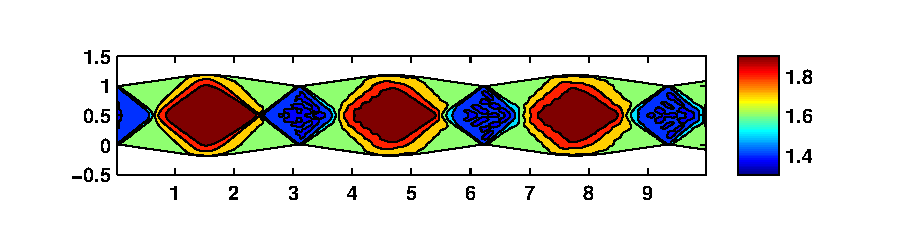
\includegraphics[width=\textwidth]{diamond_shock_train.pdf}
  \caption{Computed Mach number for an under-expanded nozzle flow, showing the diamond-shock train}
\end{figure}

\subsection{Transonic duct flow}
UCS can also be used to generate a grid that conforms to some solid body, as in the case of the transonic duct shown in Fig.~\ref{fig:shock-train-channel-flow-filmstrip}. This problem is identical to the one given by Hui\cite{Hui1999}, and is characterized by the formation of a mach stem and the resulting subsonic region and slip line. The grid simply flows through the duct, following the fluid as it conforms to the solid wall boundaries. 

It can also be seen in Fig.~\ref{fig:duct-verification} that using a stationary grid with the same code fails to capture the formation of the slip line at low grid resolutions, and also shows slightly less accurate prediction of shock locations when compared with a much higher resolution solution. UCS, on the other hand, does resolve the slip line, and makes slightly more accurate predictions of shock locations, at the cost of a less-well-resolved expansion corner.

\begin{figure}[p]
  \centering
  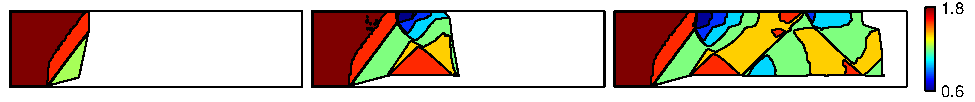
\includegraphics[width=\textwidth]{Channel_flow_filmstrip_image_mach.pdf} 
  \caption[Time-Lapse Images of Transonic Duct Flow]{Computed Mach
    number for transonic duct flow at various times, showing the
    manner in which nodes flow to fill boundaries.}
  \label{fig:shock-train-channel-flow-filmstrip}
\end{figure}

\begin{figure}[htbp]
   \centering
   \begin{subfigmatrix}{2}
      \subfigure[$h=0$, nominal grid size: $72 \times 20$]{
   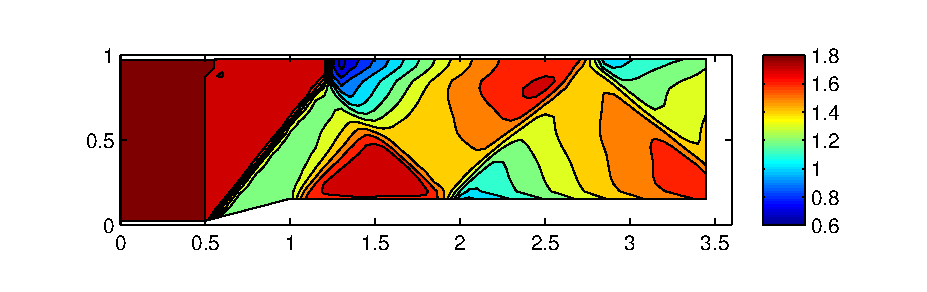
\includegraphics[width=.45\textwidth]{shock_train_contourh00p4.pdf}
   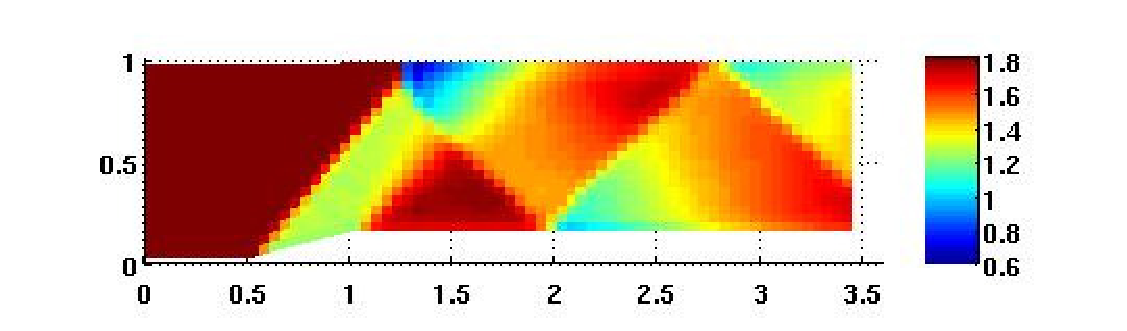
\includegraphics[width=.45\textwidth]{shock_train_surfh00p4.pdf}}
      \subfigure[$h=0.25$, nominal grid size: $72 \times 20$]{
   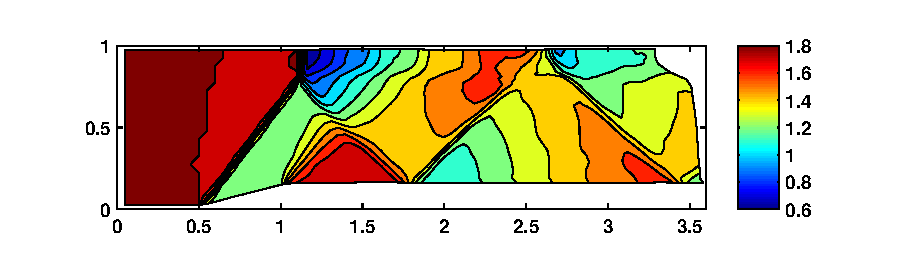
\includegraphics[width=.45\textwidth]{shock_train_contourh250p4.pdf}
   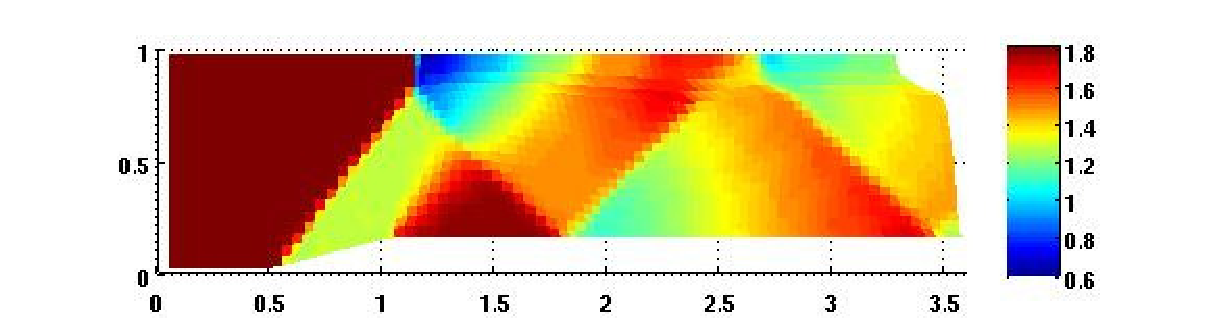
\includegraphics[width=.45\textwidth]{shock_train_surfh250p4.pdf}}
      \subfigure[$h=0$, nominal grid size: $360 \times 100$]{
   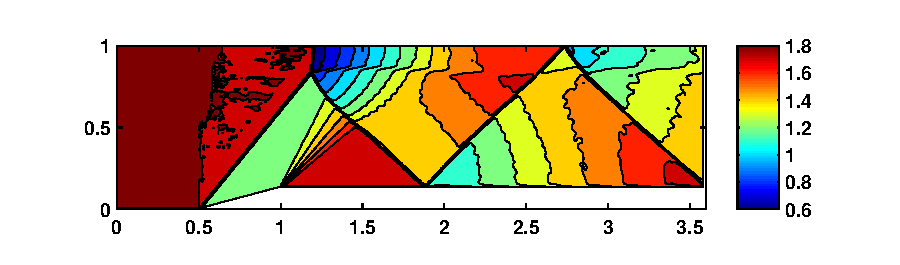
\includegraphics[width=.45\textwidth]{shock_train_contourh02p0.pdf}
   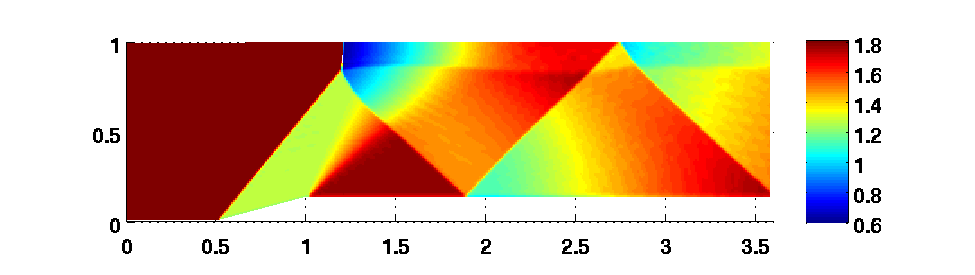
\includegraphics[width=.45\textwidth]{shock_train_surfh02p0.pdf}}
   \end{subfigmatrix}
   \caption[Accuracy Comparison Between Moving and Stationary
   grids]{Qualitative accuracy comparison between Unified ($h=0.25$)
     (b) and Eulerian ($h=0$) (a,c) simulations for a transonic duct
     flow. Notice the improved resolution of the slip line and the
     walls for the unified solution.}
   \label{fig:duct-verification}
\end{figure}

\subsection{Basic boundary-layer effects}
Many phenomena in hypersonics are a result of the interaction of the viscous boundary layer with the inviscid flow. As a result, some method of accounting for viscous effects is almost a requirement for hypersonic flows, and boundary- layer methods provide this at minimal cost.
A crude, prototypical implementation uses the turbulent, flat-plate, constant pressure formula given in Schlichting\cite{Schlichting2000}:
% MathType!MTEF!2!1!+-
% faaagCart1ev2aaaKnaaaaWenf2ys9wBH5garuavP1wzZbqedmvETj
% 2BSbqefm0B1jxALjharqqtubsr4rNCHbGeaGqiVu0Je9sqqrpepC0x
% bbL8FesqqrFfpeea0xe9Lq-Jc9vqaqpepm0xbba9pwe9Q8fs0-yqaq
% pepae9pg0FirpepeKkFr0xfr-xfr-xb9Gqpi0dc9adbaqaaeGaciGa
% aiaabeqaamaabaabaaGcbaWaaSaaaeaacqaH0oazcaWG1bWaaSbaaS
% qaaiabg6HiLcqabaaakeaacqaH9oGBaaGaeyypa0JaaGimaiaac6ca
% caaIXaGaaGinamaalaaabaGaciOuaiaacwgadaWgaaWcbaGaamiEaa
% qabaaakeaaciGGSbGaai4BaiaacEgaciGGsbGaaiyzamaaBaaaleaa
% caWG4baabeaaaaGccaWGhbWaaeWaaeaaciGGSbGaai4BaiaacEgaci
% GGsbGaaiyzamaaBaaaleaacaWG4baabeaaaOGaayjkaiaawMcaaaaa
% !48F3!
\[\frac{{\delta {u_\infty }}}{\nu } = 0.14\frac{{{{{\mathop{\rm Re}\nolimits} }_x}}}{{\log {{{\mathop{\rm Re}\nolimits} }_x}}}G\left( {\log {{{\mathop{\rm Re}\nolimits} }_x}} \right)\]
where $G$ is taken to be the limiting value of $1$. This serves as a useful proof-of-concept for the method, and is a valuable step toward future incorporation of a boundary-layer solver. In the inviscid simulation, boundary-layer effects are included by enforcing a solid wall condition that aligns with the boundary-layer displacement thickness. 

Results from one such proof-of-concept test are shown in Fig.~\ref{fig:bl-shock-train}. The presence of the boundary layer can be clearly seen in the curving of the inviscid flow in the otherwise uniform channel, as well as the formation of the oblique shock train.

\begin{figure}[p]
  \centering
  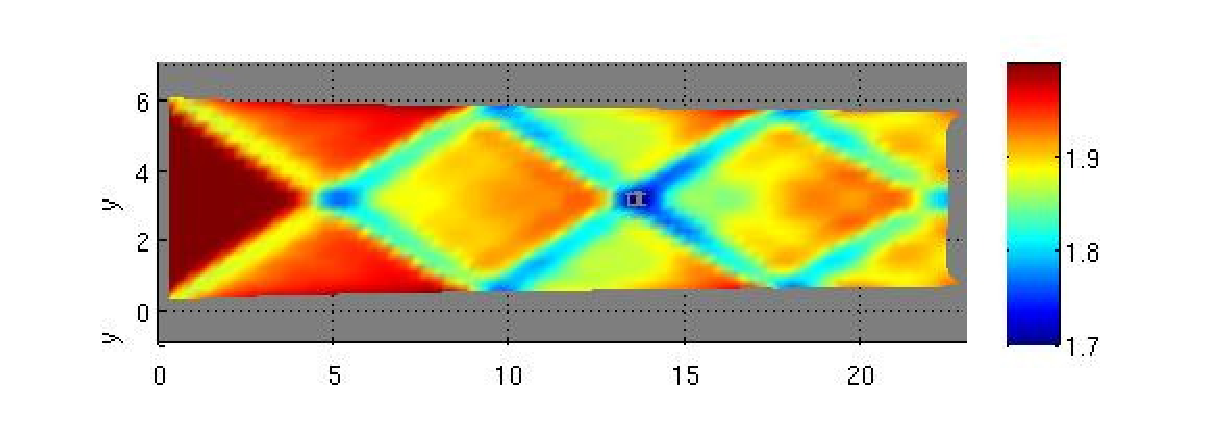
\includegraphics[width=\textwidth]{BL_shock_train2.pdf}
  \caption[Channel Flow With a Turbulent Boundary Layer]{Oblique shock train produced by a turbulent boundary layer in an otherwise uniform channel}
  \label{fig:bl-shock-train}
\end{figure}

\subsection{Model inlet}

One of the principal attractions of the unified coordinates method is the potential to represent complex flow geometries in a simple, intuitive way and without grid generation. To better illustrate this feature, a more complex inlet model was chosen, based off of publicly available sketches of the inlet of the now retired USAF F-14. This inlet is approximately two-dimensional and is designed to provide subsonic flow to the engine at freestream Mach number in the range $0 < M < 2.3$. This is accomplished through the use of internal, variable ramps, as shown in Fig.~\ref{fig:f-14-diagram}.

This is exactly the kind of problem the unified coordinates can excel at. Defining an approximate flow geometry is simple, and the automatic grid generation allows for quick solutions at different freestream conditions, and the correspondingly different inlet geometries.
An example based on the F-14 inlet is shown in Fig.~\ref{fig:f-14-flow}, but the results are only prototypical. Bleed flows, in particular, require special code features to effectively handle downstream boundaries as the grid reaches them. Further investigation into these types of problems is needed.

\begin{figure}[p]
   \centering
   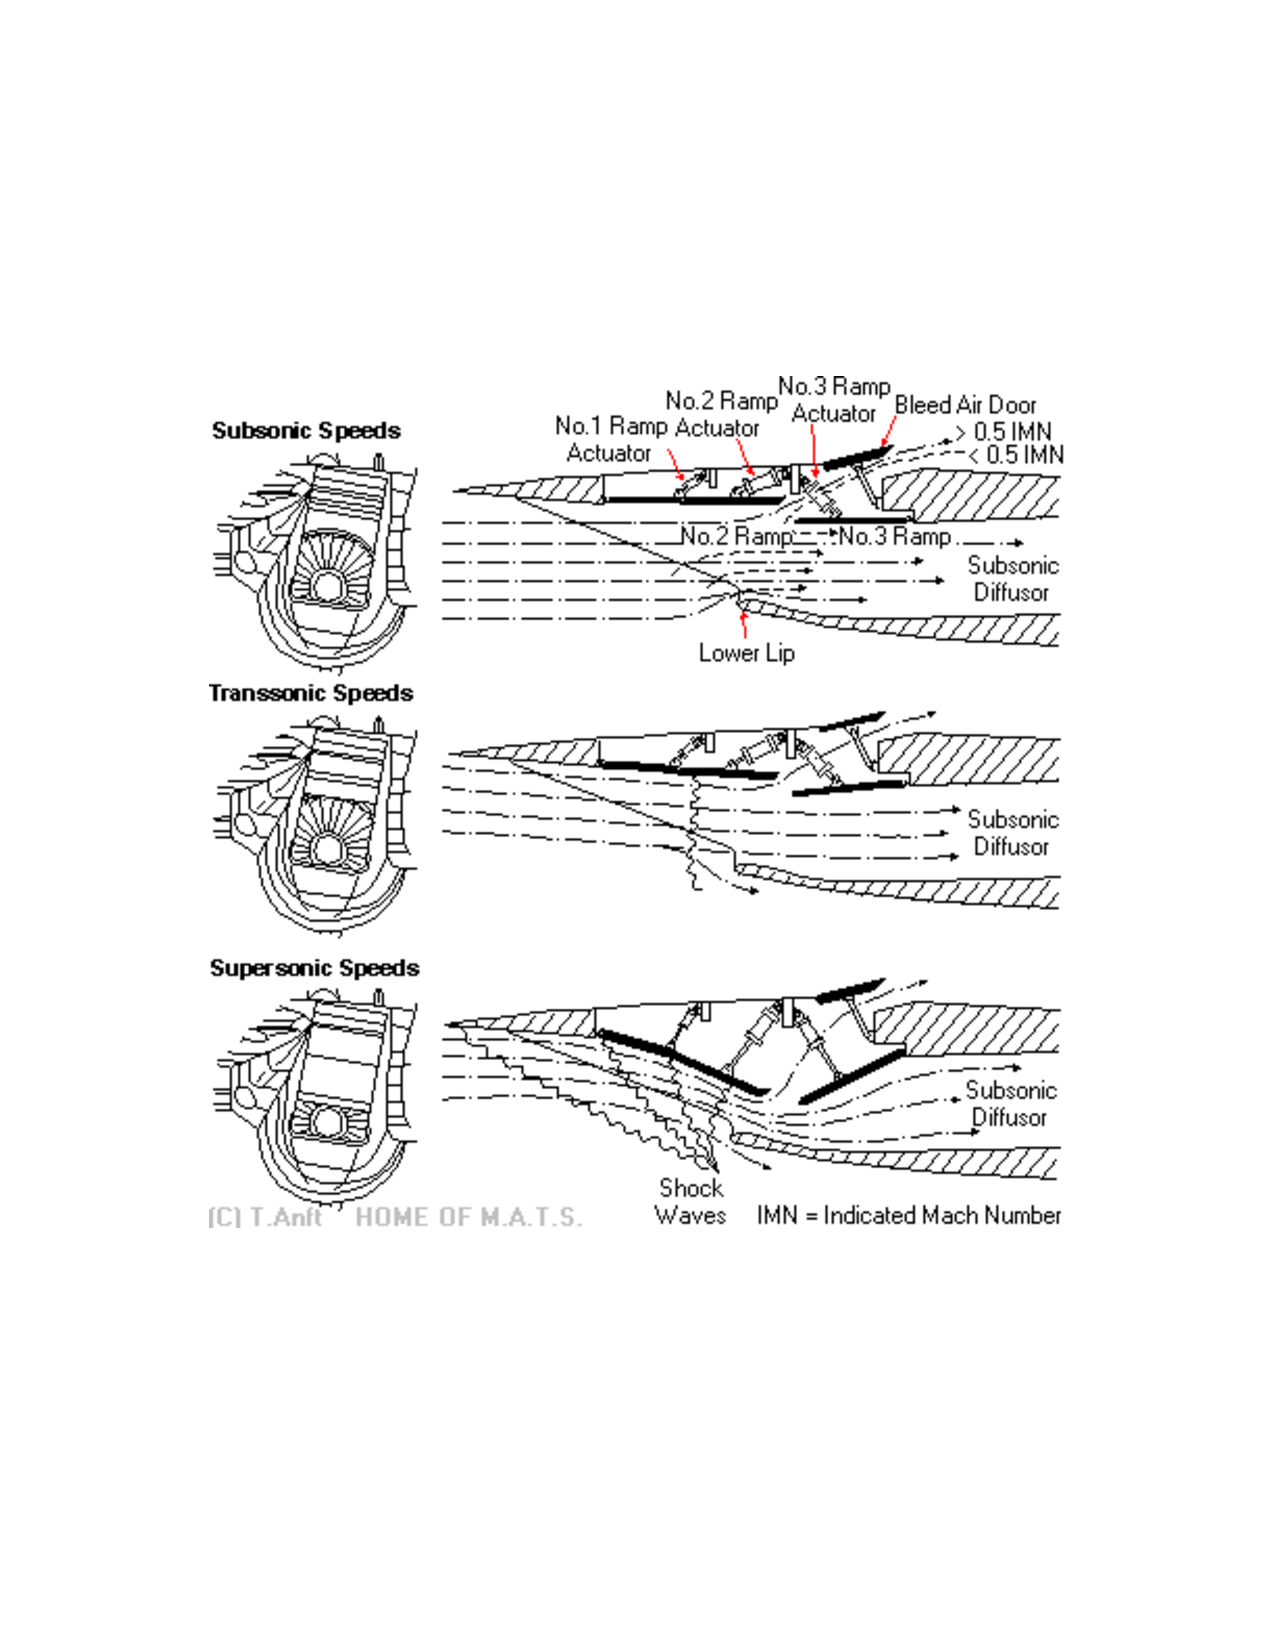
\includegraphics[width=\textwidth]{F_14_inlet_diagram.pdf}
   \vspace{-1.5in}
   \caption[Diagram of USAF F-14 Tomcat]{Diagram of the variable inlet
     geometry of the USAF F-14 Tomcat. Courtesy of: Home of M.A.T.S.,
     Available at http://www.anft.net/f-14/f14-detail-airintake.htm,
     Accessed 25 Nov 2011}
   \label{fig:f-14-diagram}
\end{figure}

\begin{figure}[htbp]
   \centering
   % \includegraphics[width=.4\textheight]{F_14_filmstrip_1.pdf}
   % \includegraphics[width=.4\textheight]{F_14_filmstrip_2.pdf}
   % \includegraphics[width=.4\textheight]{F_14_filmstrip_3.pdf}
   % \includegraphics[width=.4\textheight]{F_14_filmstrip_4.pdf}
   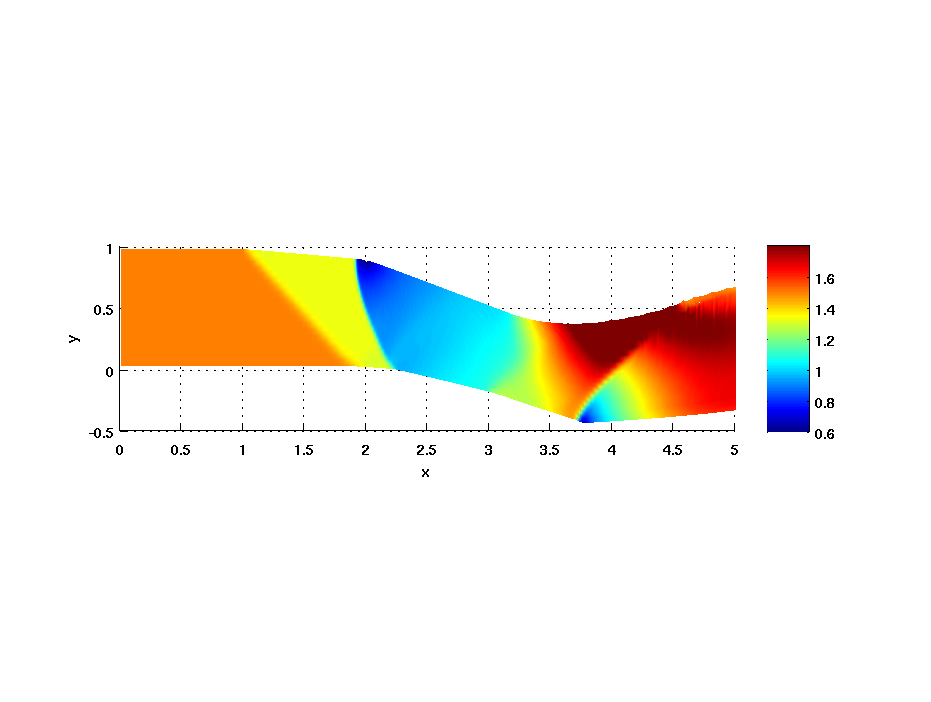
\includegraphics[width=\textwidth]{F_14_filmstrip_5clean.pdf}
   \caption[Mach Number in F-14 Inlet]{Mach number in a geometry modeled after Fig.~\ref{fig:f-14-diagram}.}
   \label{fig:f-14-flow}
\end{figure}

\section{Future Developments}
\label{sec:UCS-future}

Although UCS has shown promise for reducing the costs of CFD while raising accuracy, more work needs to be done before it can be considered a mature methodology. The preliminary results have been encouraging, but a mature code base is badly needed for both verification tests and demonstration problems. The most difficult aspects of this are the implementation of boundary conditions. Connecting the unsteady, computational coordinates in the which the UCS equations are solved with the steady, physical coordinates in which the boundary conditions are defined has proven quite challenging. 
\subsection{A first cut at better boundary conditions}
Consider a two-dimensional duct flow containing a ramp, as in Fig.~\ref{fig:shock-train-channel-flow-filmstrip}. How would one apply boundary conditions for this problem? The inflow, outflow, and top wall conditions are simple enough, and can be easily implemented as array operations: 
% MathType!MTEF!2!1!+-
% faaagCart1ev2aaaKnaaaaWenf2ys9wBH5garuavP1wzZbqedmvETj
% 2BSbqefm0B1jxALjharqqtubsr4rNCHbGeaGqiVu0Je9sqqrpepC0x
% bbL8FesqqrFfpeea0xe9Lq-Jc9vqaqpepm0xbba9pwe9Q8fs0-yqaq
% pepae9pg0FirpepeKkFr0xfr-xfr-xb9Gqpi0dc9adbaqaaeGaciGa
% aiaabeqaamaabaabaaGcbaGaiOiGhEfadaqadaqaaiaaicdacaGGSa
% GaamOAaaGaayjkaiaawMcaaiabg2da9iaahEfadaWgaaWcbaGaamyA
% aiaad6gaaeqaaOWaaeWaaeaacaaIXaGaaiilaiaadQgaaiaawIcaca
% GLPaaacaGG7aGaaGPaVlaaykW7caWHxbWaaeWaaeaacaWGUbGaamyA
% aiabgUcaRiaaigdacaGGSaGaamOAaaGaayjkaiaawMcaaiabg2da9i
% aahEfadaqadaqaaiaad6gacaWGPbGaaiilaiaadQgaaiaawIcacaGL
% PaaacaGG7aGaaGPaVlaaykW7caWHxbWaaeWaaeaacaWGUbGaamOAai
% abgUcaRiaaigdacaGGSaGaamyAaaGaayjkaiaawMcaaiabg2da9iaa
% dkhacaWGLbGaamOzaiaadYgadaqadaqaaiaahEfadaqadaqaaiaad6
% gacaWGQbGaaiilaiaadMgaaiaawIcacaGLPaaacaGGSaGaeqiUdeNa
% eyypa0JaaGimaaGaayjkaiaawMcaaaaa!69CD!
\[{\bf{W}}\left( {0,j} \right) = {{\bf{W}}_{in}}\left( {1,j} \right);\,\,{\bf{W}}\left( {ni + 1,j} \right) = {\bf{W}}\left( {ni,j} \right);\,\,{\bf{W}}\left( {nj + 1,i} \right) = refl\left( {{\bf{W}}\left( {nj,i} \right),\theta  = 0} \right)\]
where $refl$ indicates vector reflection across the wall boundary, imposing a symmetry condition at the top wall at zero degrees from horizontal.

Things become more difficult at the bottom wall. For example, one might try:

{\tt
do i = 1, ni

if(cell(i)\%x < start\_ramp .or. \&

   cell(i)\%x > end\_ramp)then
}
% MathType!MTEF!2!1!+-
% faaagCart1ev2aaaKnaaaaWenf2ys9wBH5garuavP1wzZbqedmvETj
% 2BSbqefm0B1jxALjharqqtubsr4rNCHbGeaGqiVu0Je9sqqrpepC0x
% bbL8FesqqrFfpeea0xe9Lq-Jc9vqaqpepm0xbba9pwe9Q8fs0-yqaq
% pepae9pg0FirpepeKkFr0xfr-xfr-xb9Gqpi0dc9adbaqaaeGaciGa
% aiaabeqaamaabaabaaGcbaGaaC4vamaabmaabaGaamOBaiaadMgacq
% GHRaWkcaaIXaGaaiilaiaadQgaaiaawIcacaGLPaaacqGH9aqpcaWH
% xbWaaeWaaeaacaWGUbGaamyAaiaacYcacaWGQbaacaGLOaGaayzkaa
% Gaai4oaiaaykW7caaMc8UaaC4vamaabmaabaGaamOBaiaadQgacqGH
% RaWkcaaIXaGaaiilaiaadMgaaiaawIcacaGLPaaacqGH9aqpcaWGYb
% GaamyzaiaadAgacaWGSbWaaeWaaeaacaWHxbWaaeWaaeaacaWGUbGa
% amOAaiaacYcacaWGPbaacaGLOaGaayzkaaGaaiilaiabeI7aXjabg2
% da9iaaicdaaiaawIcacaGLPaaaaaa!5844!
\[{\bf{W}}\left( {ni + 1,j} \right) = {\bf{W}}\left( {ni,j} \right);\,\,{\bf{W}}\left( {nj + 1,i} \right) = refl\left( {{\bf{W}}\left( {nj,i} \right),\theta  = 0} \right)\]

{\tt else}
% MathType!MTEF!2!1!+-
% faaagCart1ev2aaaKnaaaaWenf2ys9wBH5garuavP1wzZbqedmvETj
% 2BSbqefm0B1jxALjharqqtubsr4rNCHbGeaGqiVu0Je9sqqrpepC0x
% bbL8FesqqrFfpeea0xe9Lq-Jc9vqaqpepm0xbba9pwe9Q8fs0-yqaq
% pepae9pg0FirpepeKkFr0xfr-xfr-xb9Gqpi0dc9adbaqaaeGaciGa
% aiaabeqaamaabaabaaGcbaGaaC4vamaabmaabaGaamOBaiaadMgacq
% GHRaWkcaaIXaGaaiilaiaadQgaaiaawIcacaGLPaaacqGH9aqpcaWH
% xbWaaeWaaeaacaWGUbGaamyAaiaacYcacaWGQbaacaGLOaGaayzkaa
% Gaai4oaiaaykW7caaMc8UaaC4vamaabmaabaGaamOBaiaadQgacqGH
% RaWkcaaIXaGaaiilaiaadMgaaiaawIcacaGLPaaacqGH9aqpcaWGYb
% GaamyzaiaadAgacaWGSbWaaeWaaeaacaWHxbWaaeWaaeaacaWGUbGa
% amOAaiaacYcacaWGPbaacaGLOaGaayzkaaGaaiilaiabeI7aXjabg2
% da9iabeI7aXnaaBaaaleaacaWGYbGaamyyaiaad2gacaWGWbaabeaa
% aOGaayjkaiaawMcaaaaa!5D3A!
\[{\bf{W}}\left( {ni + 1,j} \right) = {\bf{W}}\left( {ni,j} \right);\,\,{\bf{W}}\left( {nj + 1,i} \right) = refl\left( {{\bf{W}}\left( {nj,i} \right),\theta  = {\theta _{ramp}}} \right)\]

{\tt end if

end do
}

This will certainly work. However, it quickly becomes unmanageable for complex geometries containing many different surfaces with varying reflection angles, and it is also computationally expensive, requiring conditional evaluation of each and every cell that lies on a boundary.

These problems can be managed simultaneously, by exploiting some useful features of the unified coordinate system, which does not specify anything in particular about the spatial step size in computational coordinates. In particular, it is possible to require 
% MathType!MTEF!2!1!+-
% faaagCart1ev2aaaKnaaaaWenf2ys9wBH5garuavP1wzZbqedmvETj
% 2BSbqefm0B1jxALjharqqtubsr4rNCHbGeaGqiVu0Je9sqqrpepC0x
% bbL8FesqqrFfpeea0xe9Lq-Jc9vqaqpepm0xbba9pwe9Q8fs0-yqaq
% pepae9pg0FirpepeKkFr0xfr-xfr-xb9Gqpi0dc9adbaqaaeGaciGa
% aiaabeqaamaabaabaaGcbaGaeuiLdqKaeqOVdGNaeyypa0JaeuiLdq
% Kaeq4TdGMaeyypa0JaeuiLdqKaeqOTdONaeyypa0JaaGymaaaa!3B44!
\[\Delta \xi  = \Delta \eta  = \Delta \zeta  = 1\]
It is of course possible to use any other constant as well, but a value of one is particularly convenient, because it provides a direct mapping from array indices to computational coordinates. For example, given an array of defined shape and starting coordinates 
% MathType!MTEF!2!1!+-
% faaagCart1ev2aaaKnaaaaWenf2ys9wBH5garuavP1wzZbqedmvETj
% 2BSbqefm0B1jxALjharqqtubsr4rNCHbGeaGqiVu0Je9sqqrpepC0x
% bbL8FesqqrFfpeea0xe9Lq-Jc9vqaqpepm0xbba9pwe9Q8fs0-yqaq
% pepae9pg0FirpepeKkFr0xfr-xfr-xb9Gqpi0dc9adbaqaaeGaciGa
% aiaabeqaamaabaabaaGcbaGaaC4vamaaBaaaleaacaWGPbGaamOAai
% aadUgaaeqaaOGaai4oaiaaykW7caaMc8+aaeWaaeaacqaH+oaEdaWg
% aaWcbaGaaGymaiaaigdacaaIXaaabeaakiaacYcacaaMc8UaaGPaVl
% abeE7aOnaaBaaaleaacaaIXaGaaGymaiaaigdaaeqaaOGaaiilaiaa
% ykW7caaMc8UaeqOTdO3aaSbaaSqaaiaaigdacaaIXaGaaGymaaqaba
% aakiaawIcacaGLPaaacqGH9aqpdaqadaqaaiabe67a4naaBaaaleaa
% caaIWaaabeaakiaacYcacaaMc8UaaGPaVlabeE7aOnaaBaaaleaaca
% aIWaaabeaakiaacYcacaaMc8UaaGPaVlabeA7a6naaBaaaleaacaaI
% WaaabeaaaOGaayjkaiaawMcaaaaa!5D5E!
${{\bf{W}}_{ijk}};\,\,\left( {{\xi _{111}},\,\,{\eta _{111}},\,\,{\zeta _{111}}} \right) = \left( {{\xi _0},\,\,{\eta _0},\,\,{\zeta _0}} \right)$
it is possible to write a relation allowing the computational coordinates of a cell to be determined solely from the array indices:
\begin{equation}
\label{eq:better-bcs}
% MathType!MTEF!2!1!+-
% faaagCart1ev2aaaKnaaaaWenf2ys9wBH5garuavP1wzZbqedmvETj
% 2BSbqefm0B1jxALjharqqtubsr4rNCHbGeaGqiVu0Je9sqqrpepC0x
% bbL8FesqqrFfpeea0xe9Lq-Jc9vqaqpepm0xbba9pwe9Q8fs0-yqaq
% pepae9pg0FirpepeKkFr0xfr-xfr-xb9Gqpi0dc9adbaqaaeGaciGa
% aiaabeqaamaabaabaaGcbaWaaeWaaeaacqaH+oaEcaGGSaGaeq4TdG
% MaaiilaiabeA7a6bGaayjkaiaawMcaamaaBaaaleaacaWGPbGaamOA
% aiaadUgaaeqaaOGaeyypa0ZaaeWaaeaacaWGPbGaey4kaSIaeqOVdG
% 3aaSbaaSqaaiaaicdaaeqaaOGaaiilaiaaykW7caaMc8UaamOAaiab
% gUcaRiabeE7aOnaaBaaaleaacaaIWaaabeaakiaacYcacaaMc8UaaG
% PaVlaadUgacqGHRaWkcqaH2oGEdaWgaaWcbaGaaGimaaqabaaakiaa
% wIcacaGLPaaaaaa!50BB!
{\left( {\xi ,\eta ,\zeta } \right)_{ijk}} = \left( {i + {\xi _0},\,\,j + {\eta _0},\,\,k + {\zeta _0}} \right)
\end{equation}
Using this approach, the code needs only to convert the physical coordinate representation of the boundary conditions to unsteady computational coordinates by extrapolating the grid metric from the nearest cells. This results in a loop over boundary conditions to compute updated computational coordinates, rather than a loop over cells to evaluate complex conditional statements. Once the computational coordinates of the boundary conditions are determined, they may be applied directly to the appropriate cells using the computational coordinates as defined in Eq.~\ref{eq:better-bcs}. This may be done as a simple array slice operation, with no conditional evaluation required. The principal difficulty here lies in accurately estimating the computational coordinates of boundary condition elements, and in appropriately assigning elements to grid cells. Some preliminary work in this direction has been attempted, but it remains highly experimental.

\subsection{Singular points in UCS flows}
An additional difficulty is introduced to simulations as a result of the unsteady grid used by the unified coordinate system. Considering again the ramp problem, it is quickly apparent that the location of the leading edge of the ramp has a great effect on the entire downstream flow. The same situation occurs with the two-dimensional Riemann problem in Fig. \%\%. Unfortunately, with the grid moving at an unpredictable rate, these singular points never align exactly with grid points, which automatically introduces error 
% MathType!MTEF!2!1!+-
% faaagCart1ev2aqaKnaaaaWenf2ys9wBH5garuavP1wzZbqedmvETj
% 2BSbqefm0B1jxALjharqqtubsr4rNCHbGeaGqiVu0Je9sqqrpepC0x
% bbL8FesqqrFfpeea0xe9Lq-Jc9vqaqpepm0xbba9pwe9Q8fs0-yqaq
% pepae9pg0FirpepeKkFr0xfr-xfr-xb9Gqpi0dc9adbaqaaeGaciGa
% aiaabeqaamaabaabaaGcbaGaam4tamaabmaabaGaeuiLdqKaeqOVdG
% hacaGLOaGaayzkaaaaaa!33A0!
$O\left( {\Delta \xi } \right)$ 
in the flow. Various techniques are possible to reduce this error. One is to choose time step values and grid velocities such that the singular point always coincides with a grid point. Another is to introduce an intermediate grid point that remains at the singular point. A third is to manipulate grid velocity so that the grid point at the singular point becomes stationary after the grid has been generated, similar to what Hui does with the viscous boundary layer\cite{Hui2007a}

\subsection{Accurate adherence to boundary surfaces}A final difficulty with the unified coordinates is that there is no guarantee that grid points will remain close to simulation boundaries. Since grid points are mobile, and the evolution of the grid metric depends only on the grid velocity, it is very possible for the physical coordinates of the grid to move quite far away from the actual physical boundaries, as will be discussed further in Section \ref{sec:ver-Str2-exact}. The remedy is to apply grid motion controls that take account of the actual position of the boundary conditions. It should be possible, for instance, to include a small forcing term that applies pressure to the grid to fill out boundary conditions. 
If it is important that grid cells be exactly coincident with boundary surfaces, then grid points can be constrained to move along the boundary surface itself, or the metric components can be adjusted to fit.

\subsection{Dynamic grid separation into structured blocks}
The UCS transformation itself is highly specific to structured grids, which provides many advantages, however it does complicate matters when dealing with irregular geometries. Because of the inherent flow-oriented nature of the grid, UCS is principally suited to H-type grids rather than C- or O- type. This means that the use of block-structured grids is inevitable for many kinds of flows, including flow around an embedded surface such as a wing, or flow through a round channel. In particular, flow around embedded surfaces requires the dynamic detection of the leading edge geometry and the division of the grid into separate blocks on the fly. This is made more difficult by the fact that the advancing flow at the advancing edge of the grid is typically unsteady, and it is not always apparent which grid cells should pass on which side of the embedded surface. 

\subsection{Conclusion}
Much work remains to be done with the unified coordinate system, but many of the desired new features are already under development in the latest iteration of the {\tt BACL-Streamer} code. Specific versions and their capabilities will be discussed in more detail in Chapter \ref{chpt:ver}. 